\documentclass[usepdftitle=false]{beamer}
\usetheme{Berkeley}

% introducido por mi 
\usepackage{amsmath,amsfonts,amssymb} % ecuaciones
\usepackage{siunitx}
%\usepackage{fancyhdr} % headers y footers
\usepackage{esint} % integrales cerradas
\usepackage{bbold} % para meter matriz identidad
\usepackage{graphicx} % estos dos para una figura
\usepackage[font=tiny]{caption}
\usepackage{pdfpages} % para incluir declaracion IA
\usepackage{float}
\usepackage{url}
\usepackage[export]{adjustbox}
%\usepackage[bottom]{footmisc}
\usepackage{hyperref} % to add video
\usepackage{tikz} % to generate plots 
\usepackage{setspace} % to space out text lines
\usepackage[T1]{fontenc}
\usepackage{appendixnumberbeamer}
\usetikzlibrary{decorations.markings,arrows.meta} % for big arrows
\usetikzlibrary{calc}

\usepackage[style=numeric,sorting=none, backend=biber]{biblatex}  % Load biblatex with the 'verbose' style for full citations in footnotes
\addbibresource{bibliography.bib}  % Point biblatex to your .bib file (replace with your actual filename)
%\usepackage{footbib}


\setbeamerfont{itemize/enumerate body subbody}{size=\normalsize}
\setbeamerfont{itemize/enumerate subbody}{size=\normalsize}

\tikzset{
    >={Stealth[length=3pt]}, % Standard, clean arrowhead
    % Custom style to place a single arrow at the halfway point of a path
    cleanflow/.style={
        decoration={
            markings,
            mark=at position 0.5 with {\arrow{>}}
        },
        postaction={decorate}
    },
    stable/.style={line width=1.5pt, draw=black},
    thinarc/.style={line width=0.7pt, draw=black!90},
    textlabel/.style={font=\small\selectfont, text=black}
}

\tikzset{
  flow/.style={
    decoration={
      markings,
      mark=at position #1 with {\arrow[scale=1.3]{stealth}}
    },
    postaction={decorate}
  },
  flow/.default=0.55
}

% Layer dimensions
\newcommand{\layerW}{3.0}   % width
\newcommand{\layerH}{0.45}  % height of magnetic layers
\newcommand{\barrH}{0.30}   % height of tunnel barrier

% Colors
\definecolor{ferrocolor}{RGB}{173, 216, 230}   % light blue – ferromagnet
\definecolor{barrcolor}{RGB}{255, 228, 196}    % bisque – insulating barrier

\tikzset{
  mtjlayer/.style={draw=black, thick, minimum width=\layerW cm, minimum height=\layerH cm, inner sep=0},
  barrier/.style={draw=black, thick, minimum width=\layerW cm, minimum height=\barrH cm,
                  inner sep=0, fill=barrcolor},
  magarrow/.style={-{Stealth[length=6pt, width=4pt]}, ultra thick, black},
}

\newcommand{\drawMTJ}[4]{
  % bottom ferromagnet (free layer)
  \node[mtjlayer, fill=ferrocolor] at (#1, 0) {};
  % tunnel barrier
  \node[barrier] at (#1, \layerH*0.5 + \barrH*0.5) {};
  % top ferromagnet (reference layer)
  \node[mtjlayer, fill=ferrocolor] at (#1, \layerH + \barrH) {};

  % Arrow in top (reference) layer
  \draw[magarrow]
    ({#1 - 0.55*#2}, {\layerH + \barrH})
    -- ({#1 + 0.55*#2}, {\layerH + \barrH});

  % Arrow in bottom (free) layer
  \draw[magarrow]
    ({#1 - 0.55*#3}, 0)
    -- ({#1 + 0.55*#3}, 0);

  % Layer labels
  \node[right, font=\small] at ({#1 + \layerW*0.5}, {\layerH + \barrH}) {Fixed};
  \node[right, font=\small] at ({#1 + \layerW*0.5}, {\layerH*0.5 + \barrH*0.5}) {Barrier};
  \node[right, font=\small] at ({#1 + \layerW*0.5}, 0) {Free};

  % Bit label below
  \node[font=\large\bfseries] at (#1, -0.6) {#4};
}

%\renewcommand*{\bibfont}{\tiny}
\newcommand{\xd}{\dot{x}}
\newcommand{\xdd}{\ddot{x}}
\newcommand{\yd}{\dot{y}}
\newcommand{\ydd}{\ddot{y}}
\newcommand{\bigO}{\mathcal{O}}

\newcommand{\yinyanglobe}[3]{
    \begin{scope}[rotate=#1]
        \fill[#2] (0,0) 
            arc[start angle=-90, end angle=90, radius=0.5cm] 
            arc[start angle=90, end angle=-90, radius=1cm]
            arc[start angle=90, end angle=270, radius=0.5cm] -- cycle;
            
        \fill[#3] (0, 1) circle (0.25cm);
    \end{scope}
}

\title[]{Synchronization in mechanical altermagnet}
\author{Victor Garcia}
\institute{University of Amsterdam}
\date{2025-2026}
\setbeamertemplate{footline}[frame number] %for numbering of slides
\titlegraphic{
    
\includegraphics[height=2cm]{Uva_logo.png}
    \hfill
    
\includegraphics[height=2cm]{vu_logo.png}
}

\begin{document}
\frame{\titlepage}

% \begin{frame}{Contents}
% \tableofcontents
% \end{frame}

\section{Altermagnets}

\begin{frame}{Magnetism}
\begin{itemize}
    \item Magnets break spin-rotational/time-reversal symmetry 

\begin{tikzpicture}
    % 1. Place your single PDF image
    \node[anchor=south west, inner sep=0] (image) at (0,0) {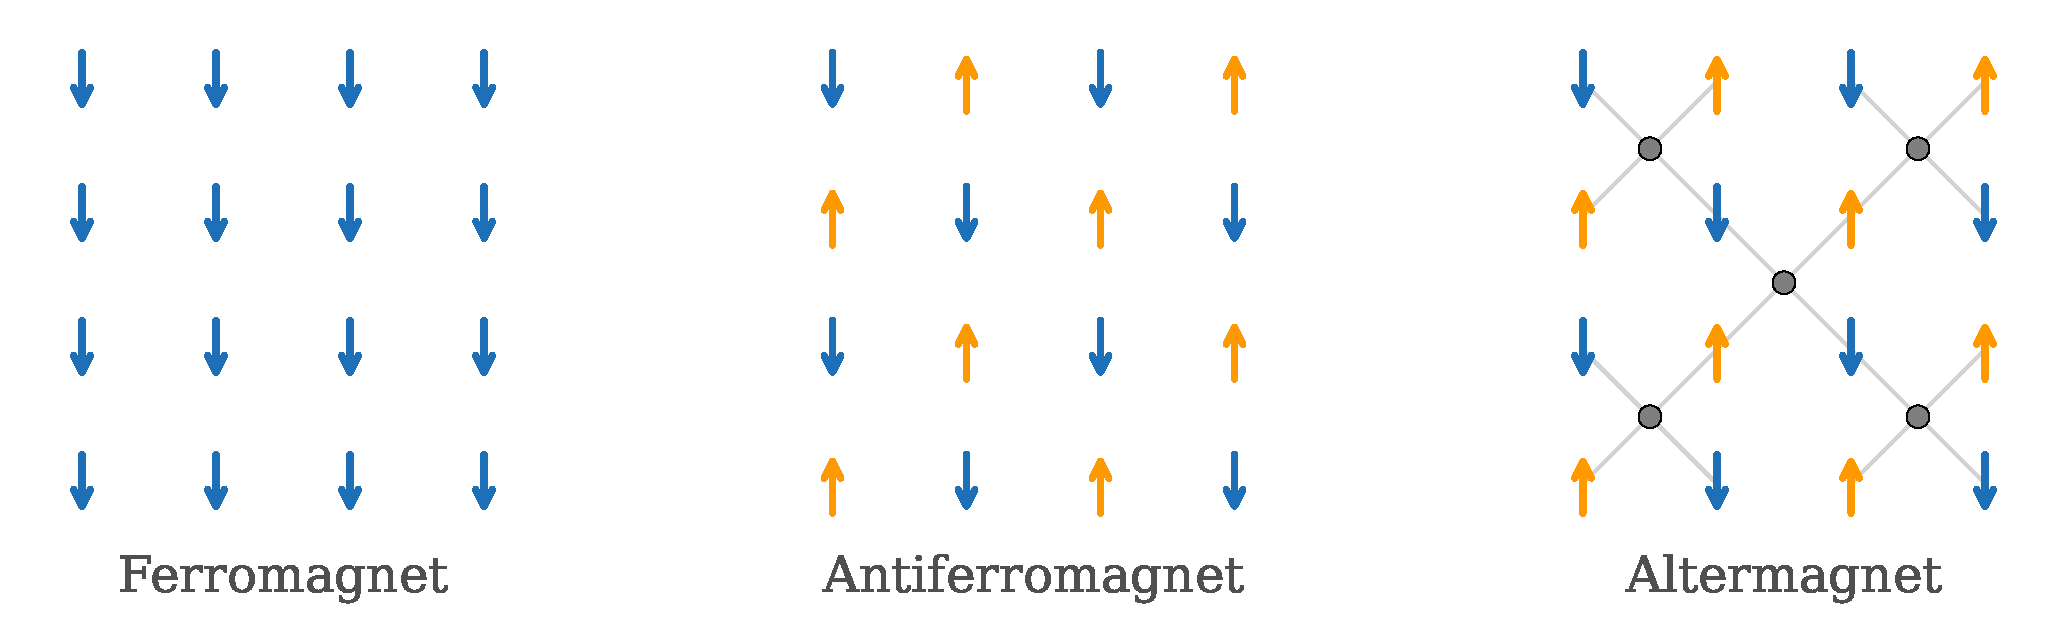
\includegraphics[width=0.9\textwidth]{magnetic_phases.pdf}};
    
    \begin{scope}[x={(image.south east)},y={(image.north west)}]
        \fill<1>[white, opacity=1.0] (0.33, 0) rectangle (1.0, 1.0);
        \fill<2>[white, opacity=1.0] (0.66, 0) rectangle (1.0, 1.0);
        \onslide<3>
    \end{scope}
\end{tikzpicture}

    \item<2-> Search for real space transformation that combined with time-reversal becomes a symmetry
    \item<3-> Discovery of altermagnets in 2022$^1$ 
\end{itemize}
\vfill
\uncover<3->{
  \scalebox{0.6}{ % Reduce el tamaño visual general
    \color{gray}
    \begin{minipage}{1.5\textwidth} % Caja con ancho suficiente para el texto
      $^1$  \fullcite{smejkal2022}
    \end{minipage}
  } 
}
\end{frame}

\begin{frame}{Magnets for storing data}
    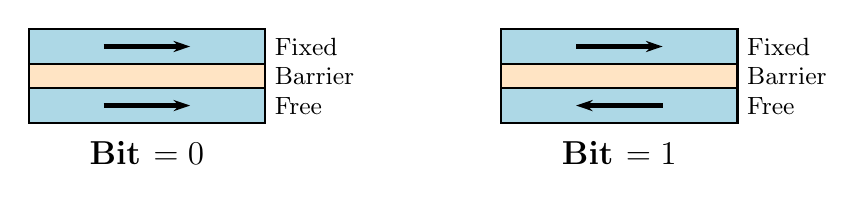
\begin{tikzpicture}
  % ---- Bit = 0  (parallel: both arrows right) ----
  \drawMTJ{0}{1}{1}{Bit $= 0$}

  % ---- Bit = 1  (antiparallel: top right, bottom left) ----
  \drawMTJ{6}{1}{-1}{Bit $= 1$}

\end{tikzpicture}
\vfill
\uncover<2->{
\begin{columns}[t]
    \begin{column}{0.5\textwidth}
        Ferromagnets:
        \begin{description}[Pro]
            \item[Pro] Large spin-splitting
            \item[Con] $M\neq 0$ 
        \end{description}
    \end{column}
    \begin{column}{0.5\textwidth}
        Antiferromagnets:
        \begin{description}[Pro]
            \item[Con] No spin-splitting
            \item[Pro] $M=0$ 
        \end{description}
    \end{column}
\end{columns}
}
\end{frame}

\begin{frame}{Altermagnets}
    \begin{alertblock}<1->{Altermagnetic symmetry}
        Real space rotation + spin-flip  denoted by $C_n\mathcal{T} $
    \end{alertblock}  
    \uncover<2->{
    \begin{block}{Properties}
        \begin{enumerate}
            \item No net magnetization $M=0$
            \item Spin-split bands $E_{\uparrow}\neq E_{\downarrow}$
            \item \alert{Spin-momentum locking} $\vec{v}_{\uparrow}\neq \vec{v}_{\downarrow}$
        \end{enumerate}
    \end{block} 
    Found in nature: MnTe, CrSb, $\text{RuO}_2$}
\end{frame}

\begin{frame}{Lieb lattice as a model altermagnet}
    \begin{columns}
        \begin{column}{0.4\textwidth}
                \begin{figure}
        
\includegraphics[scale=0.1]{yingyang.pdf}
    \end{figure}
        \end{column}
        \uncover<2->{
        \begin{column}{0.6\textwidth}
                \begin{figure}
        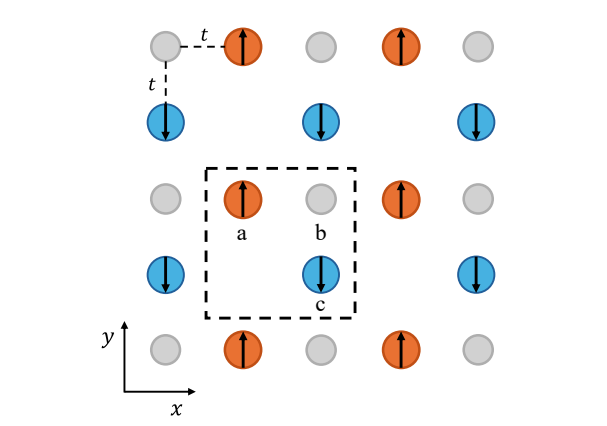
\includegraphics[width = \textwidth]{Lieb_lattice.png}
    \end{figure}
        \end{column}
        }
    \end{columns}
\uncover<2->{
\begin{itemize}
    \item 2d square lattice with 3-atom basis
    \item Symmetry: $C_4\mathcal{T}$
    \item \alert{Spin-momentum locking}
\end{itemize}         

\scalebox{0.6}{ % Reduce el tamaño visual general
    \color{gray}
    \begin{minipage}{1.5\textwidth} % Caja con ancho suficiente para el texto
      \fullcite{visser2023}
    \end{minipage}
  }
}
\end{frame}

\begin{frame}[shrink]{Generalization of altermagnetic symmetry}
    %The lattice symmetry can be generalised to other systems outside of magnetism. \\ \vspace{5mm}
     \onslide<1->{
    \begin{alertblock}{Generalization $C_4\mathcal{T} $ symmetry}
        spin $\longrightarrow$ 2-state variable
    \end{alertblock} }
    % \vfill
    \onslide<2->{
    Some examples are:
    \begin{itemize}
        \item Photon polarization $\longrightarrow$ photonic altermagnet$^1$
        \item Electric dipole $\longrightarrow$ alterelectric$^2$
        \item Oscillator chirality $\longrightarrow$ mechanical altermagnet 
    \end{itemize}  
    \centering
    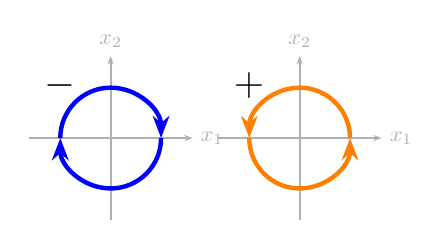
\begin{tikzpicture}[scale=0.8] % Kept at smaller scale

        % Color definition for clarity
        \definecolor{dimmed}{HTML}{B0B0B0} % Soft Grey

        % === SUBPLOT A: Clockwise (-) ===
        \begin{scope}[shift={(0,0)}]
            % Dimmed Axes (x_1 and x_2)
            \draw[->, dimmed, thick] (-1.3,0) -- (1.3,0) node[right, scale=0.8] {$x_1$};
            \draw[->, dimmed, thick] (0,-1.3) -- (0,1.3) node[above, scale=0.8] {$x_2$};
            
            % Clockwise Circle using two arcs with directional arrows
            % Top semi-circle heading clockwise (from left to right)
            \draw[-{Stealth[length=8pt, width=6pt]}, ultra thick, blue] (-0.8,0) arc (180:0:0.8);
            % Bottom semi-circle heading clockwise (from right to left)
            \draw[-{Stealth[length=8pt, width=6pt]}, ultra thick, blue] (0.8,0) arc (0:-180:0.8);
            
            % Sign in the Top Left Corner
            \node[font=\Large\bfseries, anchor=north west] at (-1.2, 1.2) {$-$};
            %\node[below, align=center] at (0,-1.5) {\small (A) Clockwise};
        \end{scope}

        % === SUBPLOT B: Counterclockwise (+) ===
        \begin{scope}[shift={(3.0,0)}]
            % Dimmed Axes (x_1 and x_2)
            \draw[->, dimmed, thick] (-1.3,0) -- (1.3,0) node[right, scale=0.8] {$x_1$};
            \draw[->, dimmed, thick] (0,-1.3) -- (0,1.3) node[above, scale=0.8] {$x_2$};
            
            % Counterclockwise Circle using two arcs with directional arrows
            % Bottom semi-circle heading counterclockwise (from left to right)
            \draw[-{Stealth[length=8pt, width=6pt]}, ultra thick, orange] (-0.8,0) arc (-180:0:0.8);
            % Top semi-circle heading counterclockwise (from right to left)
            \draw[-{Stealth[length=8pt, width=6pt]}, ultra thick, orange] (0.8,0) arc (0:180:0.8);
                
            % Sign in the Top Left Corner
            \node[font=\Large\bfseries, anchor=north west] at (-1.2, 1.2) {$+$};
            %\node[below, align=center] at (0,-1.5) {\small (B) Counterclockwise};
        \end{scope}

    \end{tikzpicture}
    \vfill
        \scalebox{0.5}{ % Reduce el tamaño visual general
            \color{gray}
            \begin{minipage}{2\textwidth} % Caja con ancho suficiente para el texto
                $^1$ \fullcite{kim2025photonicaltermagnets} \\[0.2cm]
                $^2$ \fullcite{visser2023}
            \end{minipage}
        }
    } 
\end{frame}

\section{Metamaterial setup}

\begin{frame}{Experimental setup}
         \begin{itemize}
        \setlength{\itemsep}{0.5\baselineskip}
        \item How to build a mechanical altermagnet? \pause $\longrightarrow$ Metamaterials \pause \vfill
        \item How to implement chirality?  \pause \\
        $\longrightarrow$  Non-reciprocity between two linear actuators
         \end{itemize}
    \vfill
    \begin{figure}
        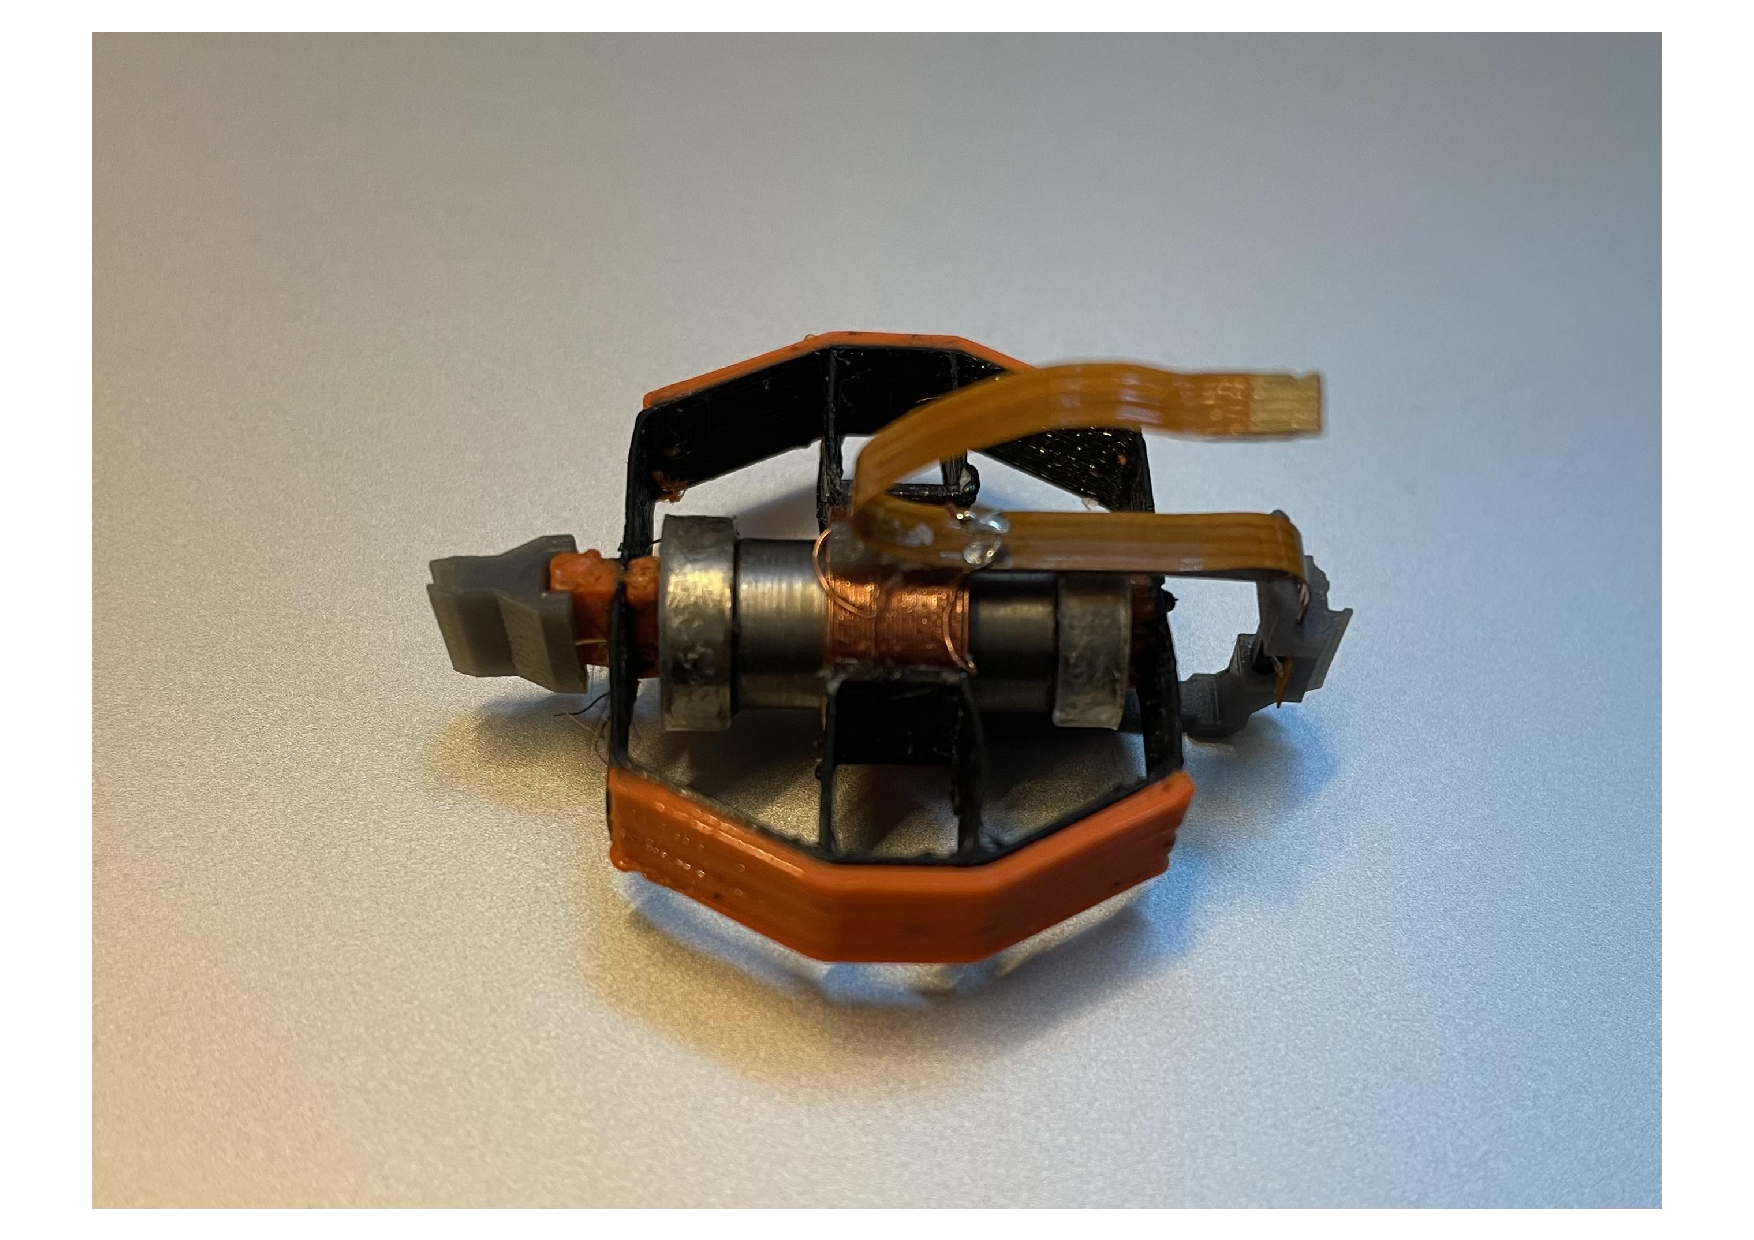
\includegraphics[width=0.5\textwidth]{Image_actuator.pdf}
    \end{figure}
\end{frame}

\begin{frame}{Non-reciprocity} 
    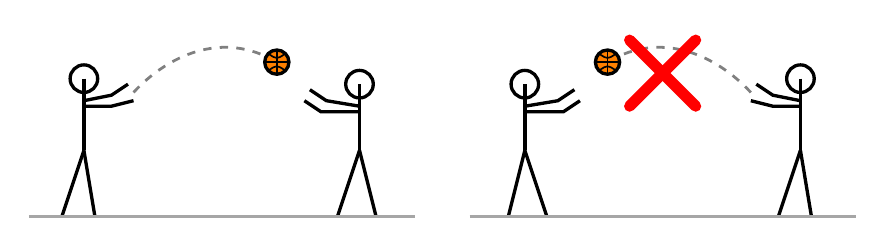
\begin{tikzpicture}[>=Stealth, line width=1.2pt, scale=0.7]

    % =========================================================================
    % SUBFIGURE A: Left to Right Pass (Success)
    % =========================================================================
    \begin{scope}[shift={(0,0)}]
        % --- Left Person (Passer) ---
        \coordinate (L-head) at (0, 2.5);
        \coordinate (L-pelvis) at (0, 1.2);
        \draw[fill=white] (L-head) circle (0.25);
        \draw (L-head) -- (L-pelvis);
        \draw (L-pelvis) -- (-0.4, 0);
        \draw (L-pelvis) -- (0.2, 0);
        \draw (0, 2.1) -- (0.5, 2.2) -- (0.8, 2.4);
        \draw (0, 2.0) -- (0.5, 2.0) -- (0.9, 2.1);

        % --- Right Person (Receiver) ---
        \coordinate (R-head) at (5, 2.4);
        \coordinate (R-pelvis) at (5, 1.2);
        \draw[fill=white] (R-head) circle (0.25);
        \draw (R-head) -- (R-pelvis);
        \draw (R-pelvis) -- (4.6, 0);
        \draw (R-pelvis) -- (5.3, 0);
        \draw (5, 2.0) -- (4.4, 2.1) -- (4.1, 2.3);
        \draw (5, 1.9) -- (4.3, 1.9) -- (4.0, 2.1);

        % --- Trajectory & Ball ---
        \coordinate (StartBall) at (0.9, 2.25);
        \coordinate (CurrentBall) at (3.5, 2.8);
        \draw[dashed, gray, line width=1pt] (StartBall) .. controls (1.5, 2.9) and (2.5, 3.4) .. (CurrentBall);
        %\draw[thin, gray, ->] (1.2, 2.4) .. controls (1.8, 2.9) .. (2.4, 3.0);
        %\draw[thin, gray, ->] (1.8, 2.8) .. controls (2.4, 3.2) .. (3.0, 3.1);

        \draw[fill=orange, draw=black] (CurrentBall) circle (0.22);
        \draw[line width=0.6pt] (3.5, 3.02) -- (3.5, 2.58); 
        \draw[line width=0.6pt] (3.28, 2.8) -- (3.72, 2.8); 
        \draw[line width=0.6pt] (3.35, 2.95) .. controls (3.5, 2.85) .. (3.65, 2.95); 
        \draw[line width=0.6pt] (3.35, 2.65) .. controls (3.5, 2.75) .. (3.65, 2.65); 

        % --- Ground Line ---
        \draw[line width=0.8pt, gray!70] (-1, 0) -- (6, 0);
    \end{scope}

    % =========================================================================
    % SUBFIGURE B: Right to Left Pass (Blocked/No Pass) - Shifted by 8 units right
    % =========================================================================
    \begin{scope}[shift={(8,0)}]
        % --- Left Person (Receiver) ---
        \coordinate (L2-head) at (0, 2.4);
        \coordinate (L2-pelvis) at (0, 1.2);
        \draw[fill=white] (L2-head) circle (0.25);
        \draw (L2-head) -- (L2-pelvis);
        \draw (L2-pelvis) -- (-0.3, 0);
        \draw (L2-pelvis) -- (0.4, 0);
        \draw (0, 2.0) -- (0.6, 2.1) -- (0.9, 2.3);
        \draw (0, 1.9) -- (0.7, 1.9) -- (1.0, 2.1);

        % --- Right Person (Passer) ---
        \coordinate (R2-head) at (5, 2.5);
        \coordinate (R2-pelvis) at (5, 1.2);
        \draw[fill=white] (R2-head) circle (0.25);
        \draw (R2-head) -- (R2-pelvis);
        \draw (R2-pelvis) -- (4.6, 0);
        \draw (R2-pelvis) -- (5.2, 0);
        \draw (5, 2.1) -- (4.5, 2.2) -- (4.2, 2.4);
        \draw (5, 2.0) -- (4.5, 2.0) -- (4.1, 2.1);

        % --- Trajectory & Ball ---
        \coordinate (StartBall2) at (4.1, 2.25);
        \coordinate (CurrentBall2) at (1.5, 2.8);
        \draw[dashed, gray, line width=1pt] (StartBall2) .. controls (3.5, 2.9) and (2.5, 3.4) .. (CurrentBall2);
        %\draw[thin, gray, ->] (3.8, 2.4) .. controls (3.2, 2.9) .. (2.6, 3.0);
        %\draw[thin, gray, ->] (3.2, 2.8) .. controls (2.6, 3.2) .. (2.0, 3.1);

        \draw[fill=orange, draw=black] (CurrentBall2) circle (0.22);
        \draw[line width=0.6pt] (1.5, 3.02) -- (1.5, 2.58); 
        \draw[line width=0.6pt] (1.28, 2.8) -- (1.72, 2.8); 
        \draw[line width=0.6pt] (1.35, 2.95) .. controls (1.5, 2.85) .. (1.65, 2.95); 
        \draw[line width=0.6pt] (1.35, 2.65) .. controls (1.5, 2.75) .. (1.65, 2.65); 

        % --- Ground Line ---
        \draw[line width=0.8pt, gray!70] (-1, 0) -- (6, 0);

        % --- BIG RED BLOCKING CROSS ---
        \coordinate (CrossCenter) at (2.5, 2.6);
        \draw[line width=4pt, red, cap=round] ($(CrossCenter)+(-0.6,-0.6)$) -- ($(CrossCenter)+(0.6,0.6)$);
        \draw[line width=4pt, red, cap=round] ($(CrossCenter)+(-0.6,0.6)$) -- ($(CrossCenter)+(0.6,-0.6)$);
    \end{scope}

\end{tikzpicture}
    \begin{itemize} 
        \item Asymmetry in interaction \pause
        \item Odd elasticity: $F_1 = k_a x_2 \quad F_2=-k_a x_1$
                \begin{alertblock}{Experimental control parameter}
        Activity/gain $k_a$
    \end{alertblock}  
        \item No conservation of energy \begin{description}
            \item[1] Active
            \item[2] Non-hermitian
        \end{description}
    \end{itemize}
\end{frame}

\begin{frame}{Non-reciprocity leads to limit cycles}
        EOM of two non-reciprocally coupled actuators:
    \begin{align*}
        \xdd_1 +k_0x_1 +  \gamma \xd_1 + k_cx_1^3 + k_ax_2 = 0 \\ 
        \xdd_2 +k_0x_2 +  \gamma \xd_2 + k_cx_2^3 - k_ax_1 = 0 
    \end{align*}
    \onslide<2->{
    \begin{columns}
            \begin{column}{0.35\textwidth}
        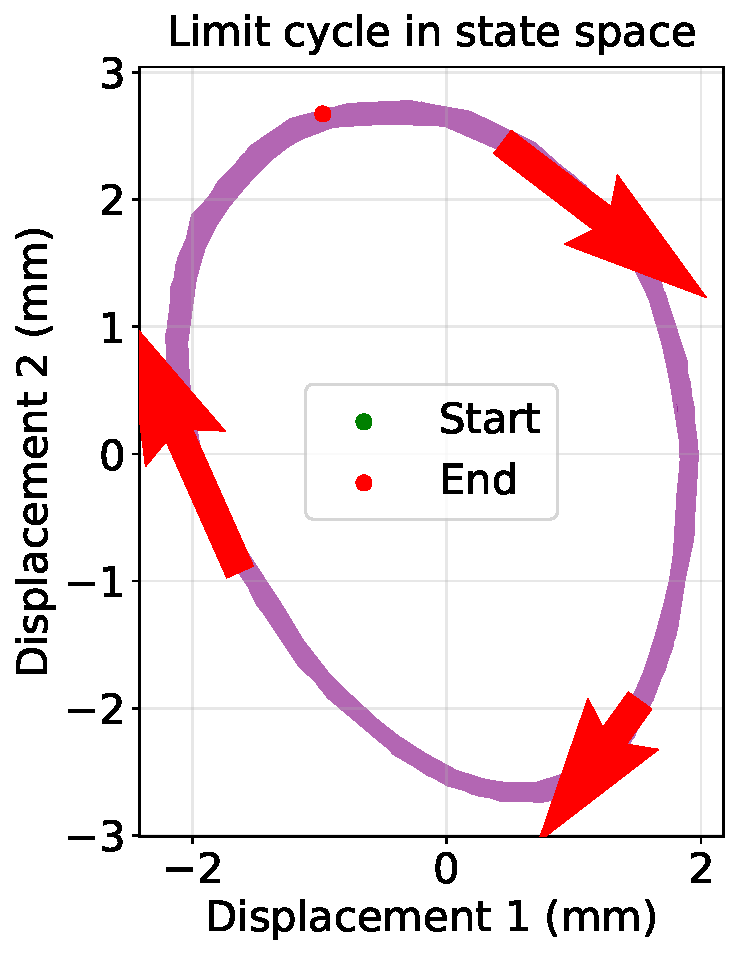
\includegraphics[width=\textwidth]{limit_cycle_example.pdf}
    \end{column}
        \begin{column}{0.6\textwidth}
                \begin{minipage}{\textwidth}
        \hfill
 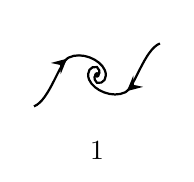
\begin{tikzpicture}[scale=0.4]
    \useasboundingbox (-2.2, -2.5) rectangle (2.2, 1.5);
        %\draw[red, dashed] (current bounding box.south west) rectangle (current bounding box.north east);
  % Trajectory from bottom-left, spirals into fixed point
  \draw[thick, flow=0.45]
    (-2.0,-1.0) .. controls (-1.5,-0.8) and (-1.2, 0.4) ..
    (-0.9, 0.55) .. controls (-0.5, 0.75) and ( 0.1, 0.5) ..
    ( 0.25, 0.15) .. controls ( 0.35,-0.1) and ( 0.2,-0.3) ..
    ( 0.0,-0.25) .. controls (-0.15,-0.1) and (-0.05, 0.0) ..
    (-0.02, 0.0);

  % Second trajectory from top-right, spirals into fixed point
  \draw[thick, flow=0.45]
    ( 2.0, 1.0) .. controls ( 1.5, 0.8) and ( 1.2,-0.4) ..
    ( 0.9,-0.55) .. controls ( 0.5,-0.75) and (-0.1,-0.5) ..
    (-0.25,-0.15) .. controls (-0.35, 0.1) and (-0.2, 0.3) ..
    ( 0.0, 0.25) .. controls ( 0.15, 0.1) and ( 0.05, 0.0) ..
    ( 0.02, 0.0);

  % Stable fixed point (filled dot)
  \filldraw (0,0) circle (2pt);

  % Label
  \node at (0,-2.4) {1};

\end{tikzpicture}
%\hspace{0cm}
Hopf
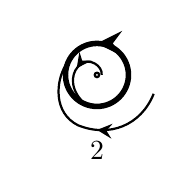
\begin{tikzpicture}[scale=0.4]
        \useasboundingbox (-2.2, -2.5) rectangle (2.2, 1.5);
        %\draw[red, dashed] (current bounding box.south west) rectangle (current bounding box.north east);
  % Stable limit cycle (thicker, radius 1 cm)
  \draw[line width=2pt, flow=0.25] (0,0) circle (1.0cm);

  % Trajectory spiralling outward from near origin to limit cycle
  \draw[thick, flow=0.5]
    (0.15, 0.0)
    .. controls ( 0.18, 0.30) and (-0.25,  0.55) ..
    (-0.5,  0.35)
    .. controls (-0.80, 0.15) and (-0.90, -0.35) ..
    (-0.5, -0.80);   % ends near the circle r ≈ 1

  % Trajectory spiralling inward from outside to limit cycle
  \draw[thick, flow=0.45]
    ( 1.80,-0.60)
    .. controls ( 1.40,-1.60) and ( 0.40,-2.00) ..
    (-0.60,-1.60)
    .. controls (-1.40,-1.20) and (-1.30,-0.20) ..
    (-1.00, 0.30);   % ends near the circle r ≈ 1

  % Unstable fixed point (open dot)
  \filldraw[fill=white, draw=black, thick] (0,0) circle (2pt);

  % Label
  \node at (0,-2.4) {2};

\end{tikzpicture}
    \end{minipage}
    \begin{enumerate}
    \item[1] If $|k_a|<\gamma \sqrt{k_0}$, oscillations die
    \item[2] If $|k_a|>\gamma \sqrt{k_0}$, stable limit cycles, with chirality \begin{enumerate}
        \item[a] $k_a>0$ counterclockwise 
        \item[b] $k_a<0$ clockwise 
    \end{enumerate}
    \end{enumerate}
        \end{column}
    \end{columns}
    }
\end{frame}

\begin{frame}{Experimental results of one unit}
    \begin{columns}
    \begin{column}{0.5\textwidth}
        \begin{figure}
            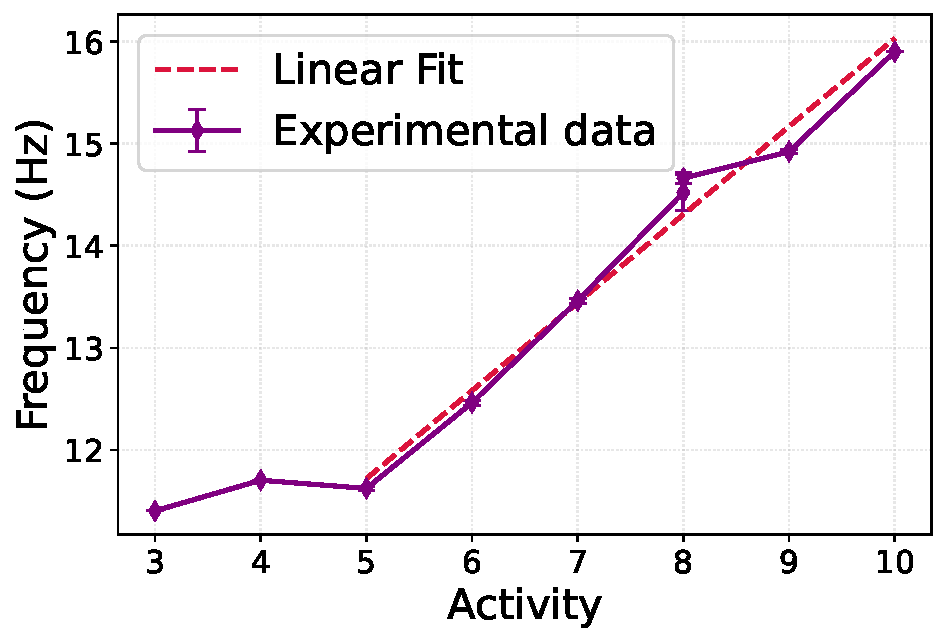
\includegraphics[width = \textwidth]{linear_frequency_scaling_one_node.pdf}
        \end{figure}
        \vfill
        Theory predicts: $\omega = \frac{k_a}{\gamma}$
    \end{column} 
    \uncover<2->{
    \begin{column}{0.5\textwidth}
        \begin{figure}
            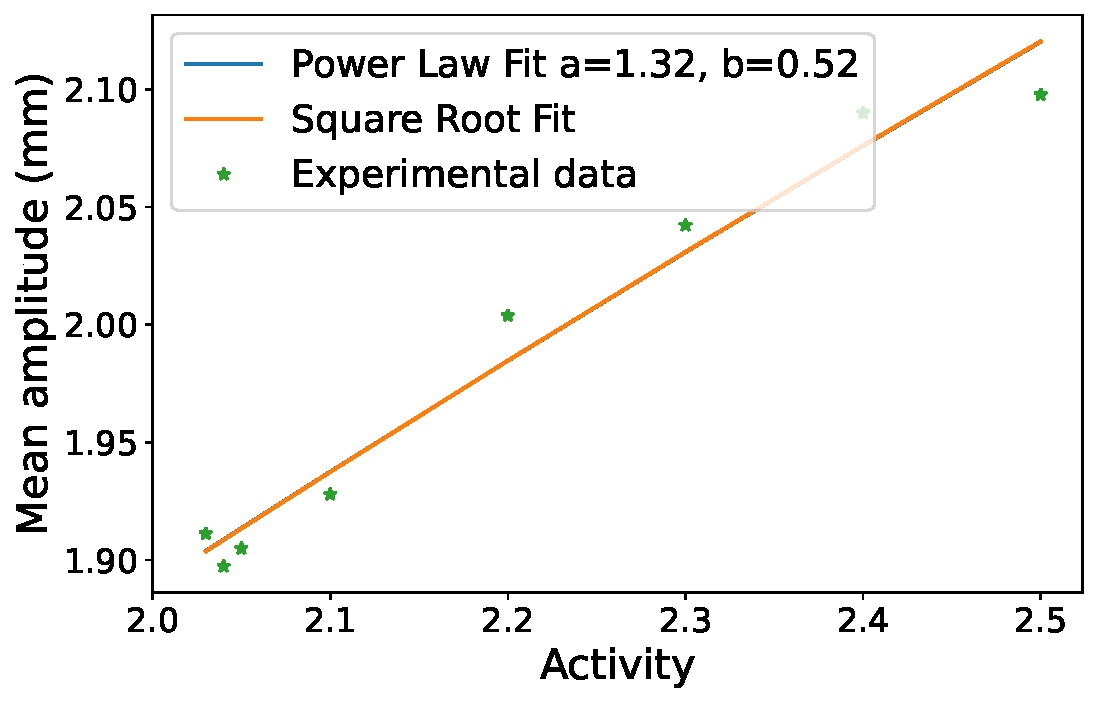
\includegraphics[width = \textwidth]{amplitude_scaling_Hopf.pdf}
        \end{figure}
        \vfill
        $R \sim \sqrt{\frac{2k_a^c}{k_c\gamma^2}(k_a-k_a^c)}$
    \end{column}
    }
    \end{columns}
\end{frame}

% \begin{frame}{Experimental results of one unit}
%         \begin{minipage}[t]{0.6\textwidth}
%     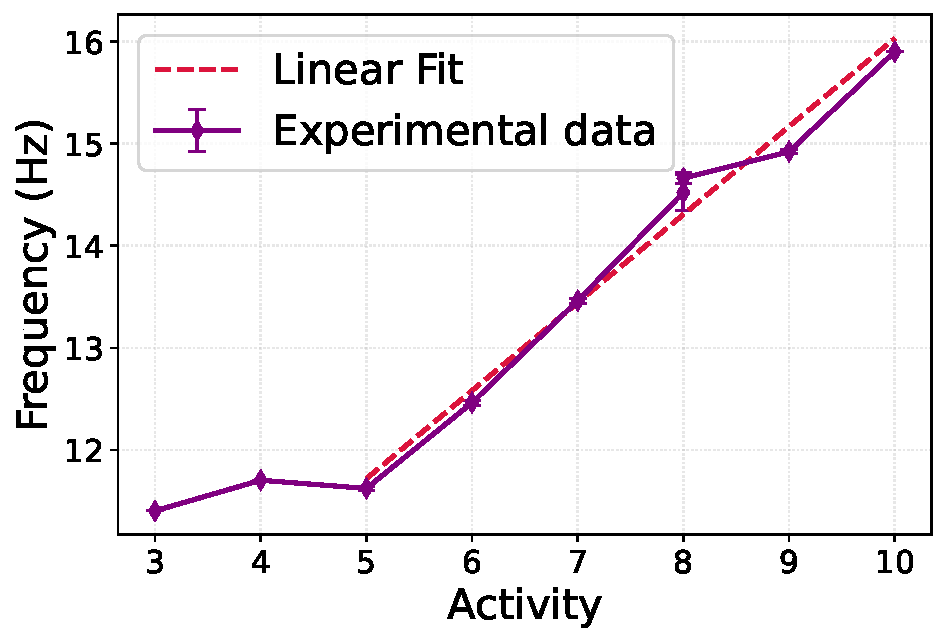
\includegraphics[height=0.5\textheight]{linear_frequency_scaling_one_node.pdf}
%     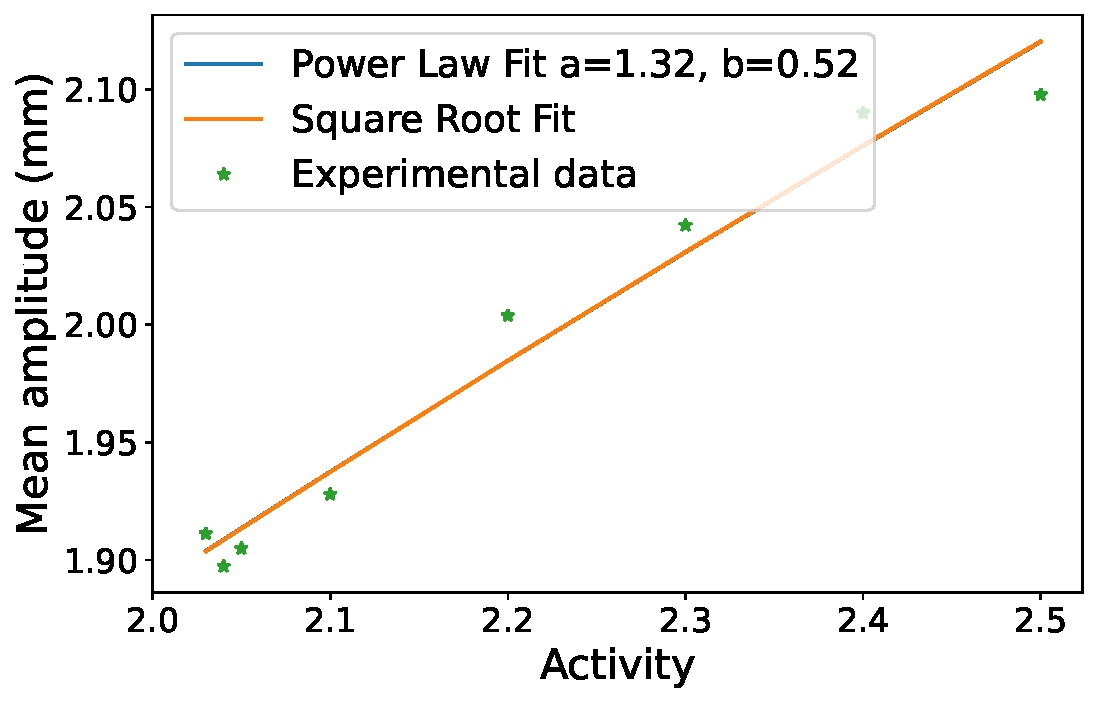
\includegraphics[height=0.5\textheight]{amplitude_scaling_Hopf.pdf}
%         \end{minipage}
%         \begin{minipage}[t]{0.38\textwidth}
%             \vfill

%                 Theory predicts: 

%             \vfill

%             $\omega = \frac{k_a}{\gamma}$

%             \vfill

%             $R \sim \sqrt{\frac{2k_a^c}{k_c\gamma^2}(k_a-k_a^c)}$

%             \vfill
%         \end{minipage}
% \end{frame}

% \begin{frame}{Amplitude of one unit}
%         \begin{figure}
%         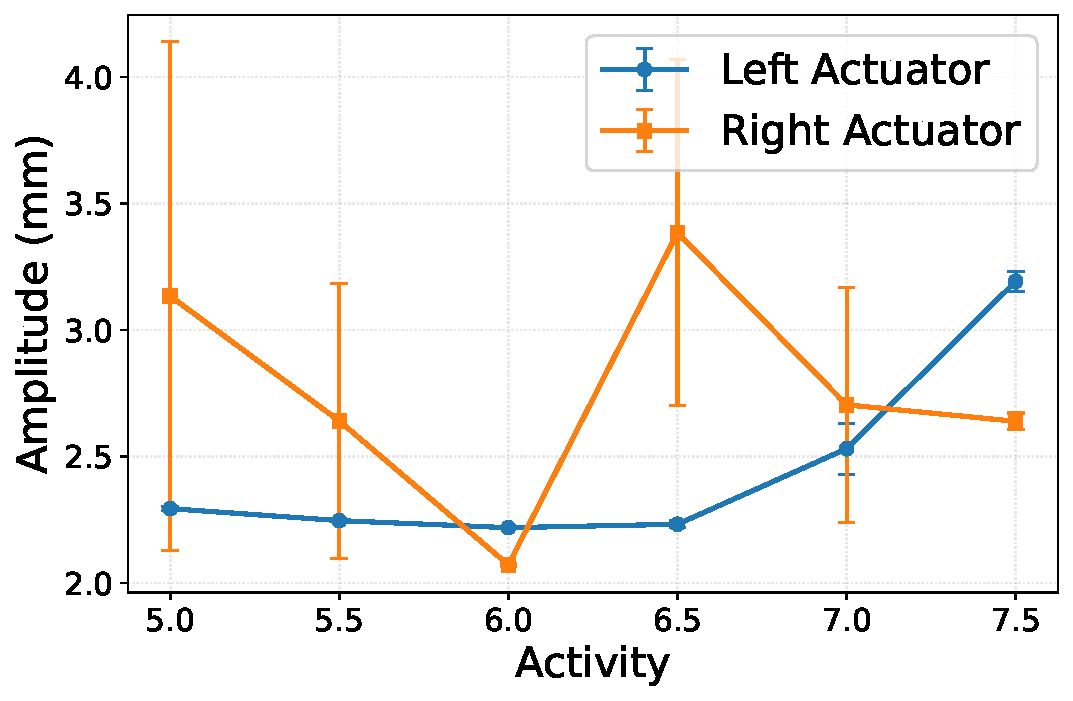
\includegraphics[width = 0.8\textwidth]{radius_one_node.pdf}
%     \end{figure}
%     \begin{itemize}
%         \item Limit cycle amplitude is inconsistent
%     \end{itemize}
% \end{frame}

\begin{frame}{Experimental setup}
    Next: adding more units 
        \begin{columns}
        \begin{column}{0.6\textwidth} 
    \begin{itemize}
        \setlength{\itemsep}{\baselineskip}
        \item Neighbour interactions through elastic band
        \uncover<2->{
        \item Different geometries 
    \begin{enumerate}
        \setlength{\itemsep}{0.1\baselineskip}
        \item One unit: two actuators
        \item Two units
        \item 1d chain
        \item Cross cell
        \item Lieb lattice
    \end{enumerate}
        }
    \end{itemize}
        \end{column}
        \uncover<2->{
        \begin{column}{0.4\textwidth}
           \href{run:MicrosoftTeams-video_2.mp4}{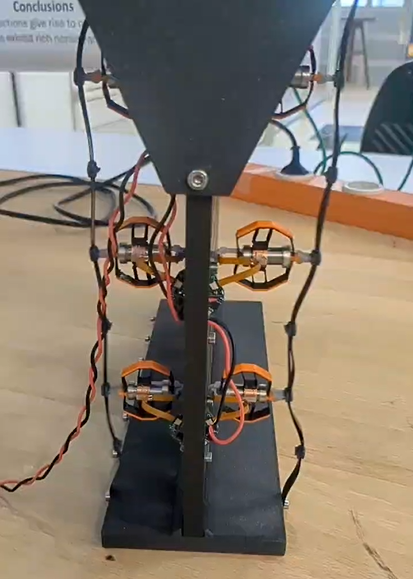
\includegraphics[width=\textwidth]{first_frame_video_exp_setup_slowmo.PNG}} 
        \end{column}
        }
        \end{columns}
\end{frame}

\begin{frame}{Synchronization}
    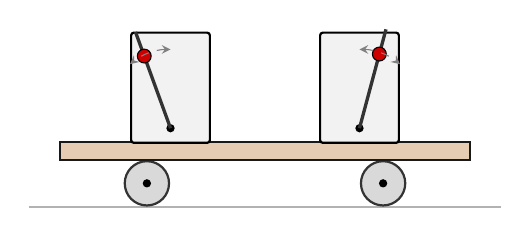
\begin{tikzpicture}[
    scale=1, transform shape,
    >=stealth,
    % Styles for the components
    roller/.style={circle, draw=black!80, fill=gray!30, thick, minimum size=16pt},
    board/.style={rectangle, draw=black!90, fill=brown!40, thick, minimum size=6pt},
    metronome/.style={rectangle, draw=black, fill=gray!10, thick, rounded corners=1pt},
    bob/.style={circle, fill=red!80!black, draw=black, minimum size=5pt, inner sep=0pt}
]

    % =========================================================================
    % 1. THE BASE: ROLLER CYLINDERS & COUPLING MOTION
    % =========================================================================
    % Ground line
    \draw[thick, gray!60] (-3, -0.3) -- (3, -0.3);

    % Two Cylindrical Rollers
    \node[roller] (left_roll) at (-1.5, 0) {};
    \node[roller] (right_roll) at (1.5, 0) {};
    
    % Tiny center dots for the cylinders
    \fill[black] (left_roll.center) circle (1.5pt);
    \fill[black] (right_roll.center) circle (1.5pt);

    % Coupling horizontal motion arrows for the board/rollers
    \draw[<->, line width=1pt, gray!80] (-2.2, 0.4) -- (-1.7, 0.4);
    \draw[<->, line width=1pt, gray!80] (1.7, 0.4) -- (2.2, 0.4);

    % =========================================================================
    % 2. THE COUPLING BOARD
    % =========================================================================
    % Stretches across both rollers
    \node[board, minimum width=5.2cm, anchor=south] (the_board) at (0, 0.28) {};


    % =========================================================================
    % 3. METRONOME 1 (Left Side - Tilted Left)
    % =========================================================================
    \begin{scope}[shift={(-1.2, 0.5)}]
        % Base/Body housing
        \node[metronome, minimum width=1.0cm, minimum height=1.4cm, anchor=south] (m1) at (0,0) {};
        
        % Pivot point location
        \coordinate (p1) at (0, 0.2);
        \fill[black] (p1) circle (1.5pt);
        
        % Long Pendulum Bar (Tilted left by 20 degrees)
        \draw[line width=1.2pt, draw=black!80] (p1) -- ++(110:1.3) coordinate (tip1);
        % Weighted Bob
        \node[bob] at ($(p1)!0.75!(tip1)$) {};
        
        % Motion arc indicator
        \draw[<->, dashed, thin, gray] (0, 1.2) arc (90:130:0.8);
    \end{scope}


    % =========================================================================
    % 4. METRONOME 2 (Right Side - Tilted Right)
    % =========================================================================
    \begin{scope}[shift={(1.2, 0.5)}]
        % Base/Body housing
        \node[metronome, minimum width=1.0cm, minimum height=1.4cm, anchor=south] (m2) at (0,0) {};
        
        % Pivot point location
        \coordinate (p2) at (0, 0.2);
        \fill[black] (p2) circle (1.5pt);
        
        % Long Pendulum Bar (Tilted right by 15 degrees)
        \draw[line width=1.2pt, draw=black!80] (p2) -- ++(75:1.3) coordinate (tip2);
        % Weighted Bob
        \node[bob] at ($(p2)!0.75!(tip2)$) {};
        
        % Motion arc indicator
        \draw[<->, dashed, thin, gray] (0, 1.2) arc (90:50:0.8);
    \end{scope}

\end{tikzpicture} \\
\uncover<2->{
    Requirements:
    \begin{itemize}
        \item Autonomous oscillators
        \item Interactions: via elastic band $\longrightarrow$ weak
        \item Parameter proximity
    \end{itemize}
}
    \vfill 
    \begin{columns}
        \uncover<3->{
        \begin{column}{0.5\textwidth}
           Adler equation:
\begin{equation*}
    \frac{d \varDelta \phi }{dt} = \underbrace{\varDelta \omega}_{\omega_1 - \omega_2} - K \sin(\varDelta \phi)
\end{equation*}
        \end{column}
        }
        \uncover<4->{
        \begin{column}{0.5\textwidth}
            \begin{description}
    \item[$\varDelta \omega < K$] Synchronization
    \item[$\varDelta \omega > K$] Chaos 
\end{description}
        \end{column}
        }
    \end{columns}
\end{frame}

\section{Two units}

\begin{frame}{Two units with same chirality synchronize}
        \begin{figure}
        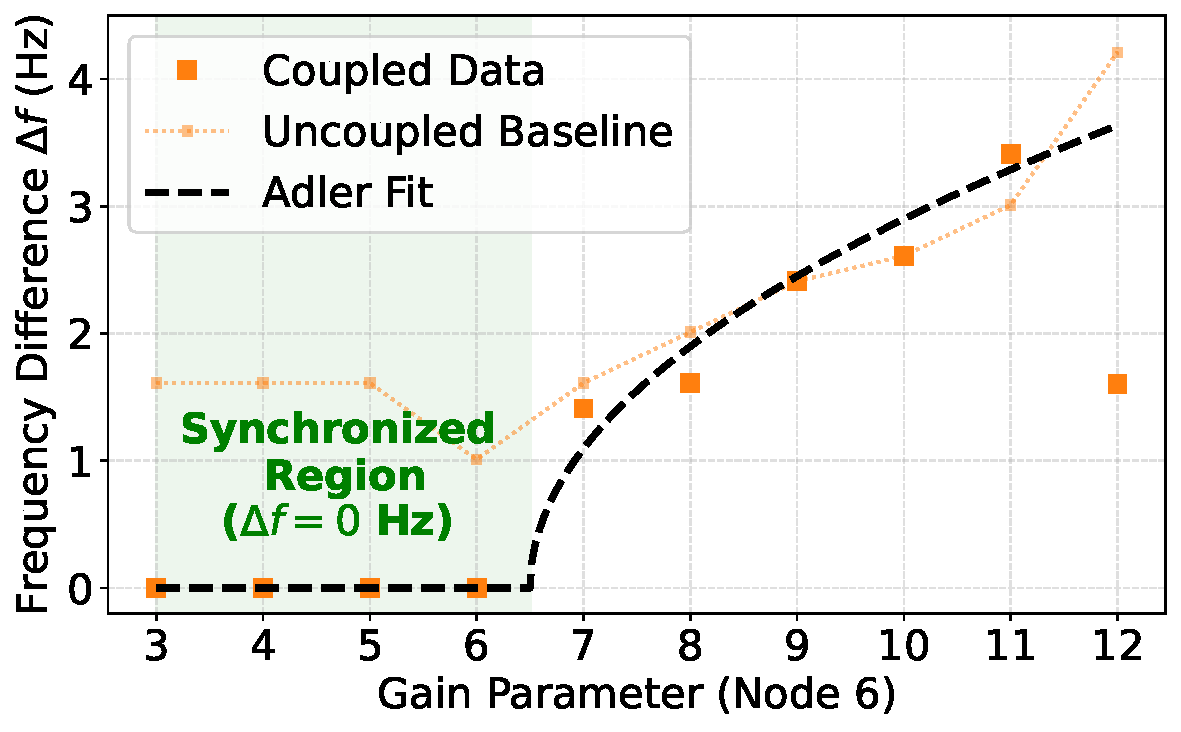
\includegraphics[width=0.9\textwidth]{sync_region_freq_diff.pdf}
    \end{figure}
    \begin{columns}
        \begin{column}{0.7\textwidth}
            If activity difference or detuning is large, they stop synchronizing
        \end{column}
        \begin{column}{0.3\textwidth}
            \begin{figure}
        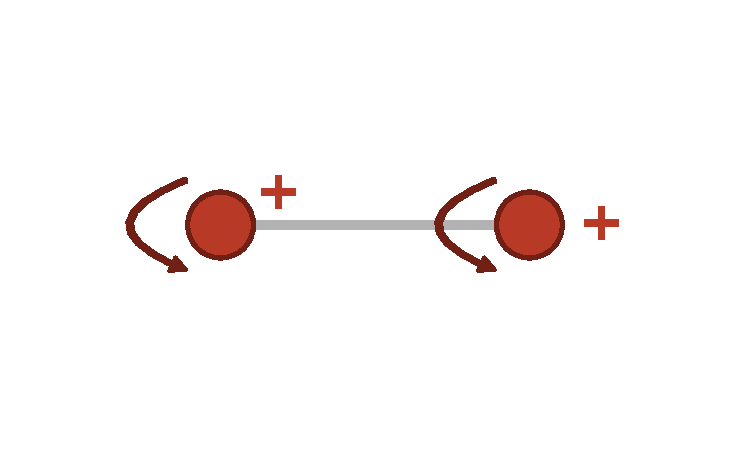
\includegraphics[right, scale=0.2]{diagram_2_units_same_chir_straight.pdf}
        \end{figure} 
        \end{column}
    \end{columns}
    % \begin{alertblock}{}
    %     Units with same chirality synchronize
    % \end{alertblock}
\end{frame}

\begin{frame}{Units with opposite chirality do not synchronize}
    \begin{columns}[t]
        \begin{column}{0.15\textwidth}
            \begin{figure}
                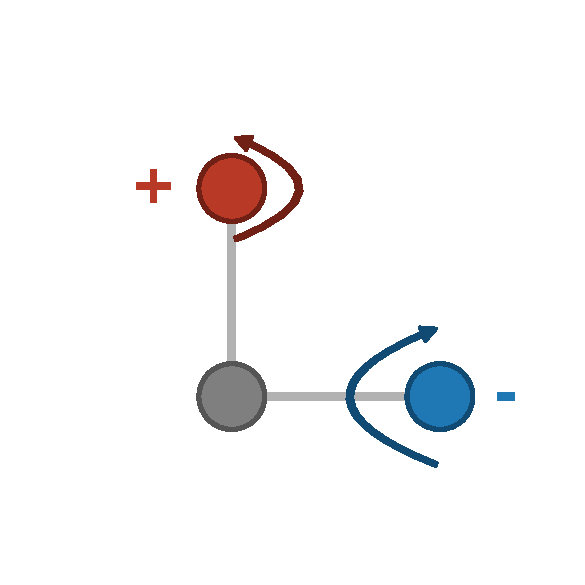
\includegraphics[scale=0.2]{diagram_2units_am_cell.pdf}
            \end{figure}  
        \end{column}
        \begin{column}{0.85\textwidth}
            \begin{figure}
                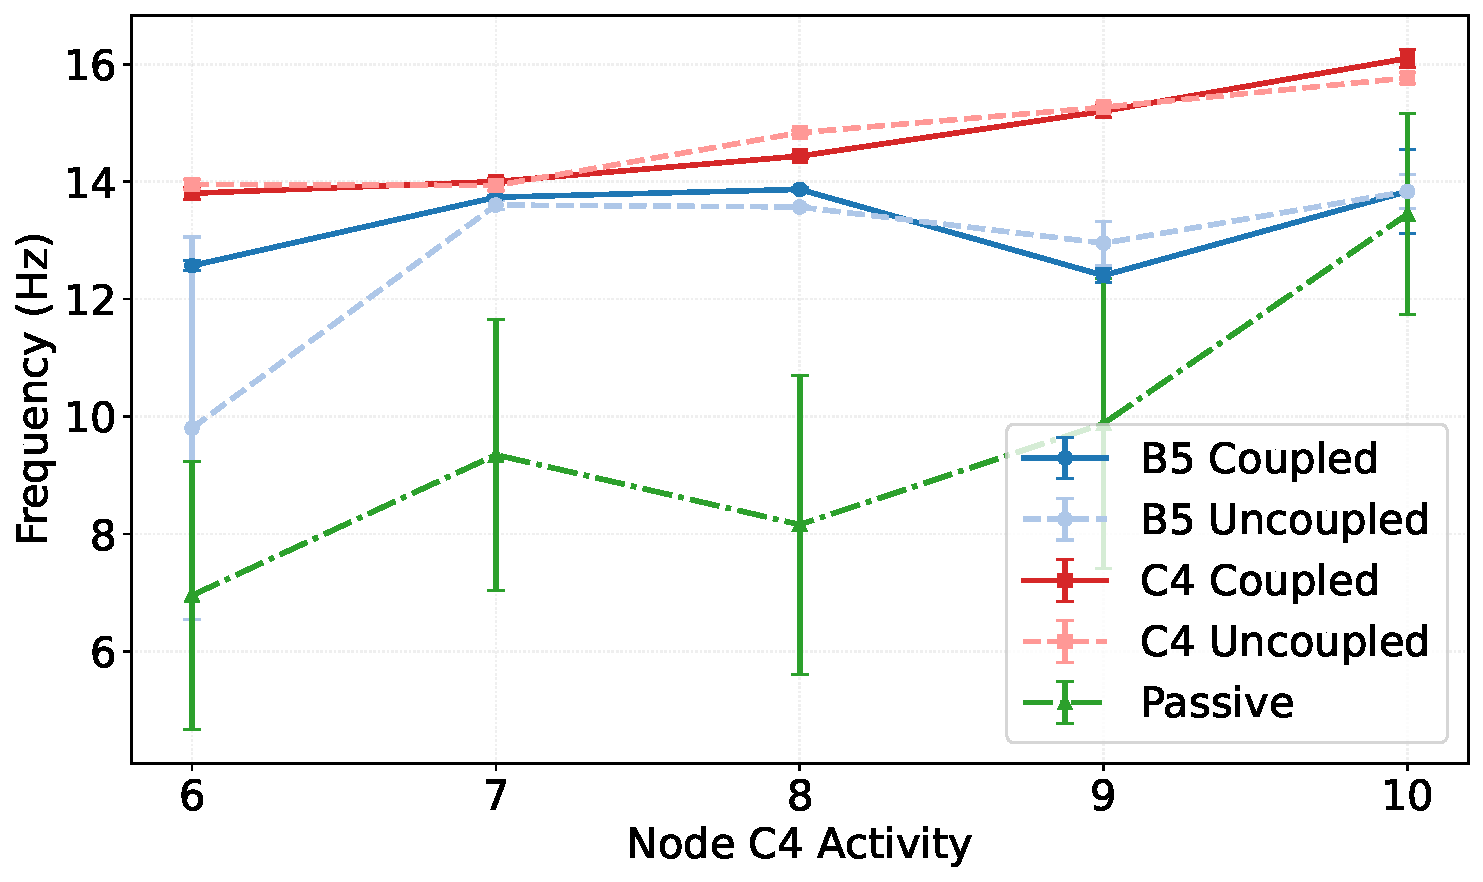
\includegraphics[width=\textwidth]{two_nodes_opp_chir.pdf}
            \end{figure}
        \end{column}
    \end{columns}
    \vfill
    Passive unit introduces an extra mode that absorbs energy
\end{frame}

\section{Chain}

\begin{frame}{1d chain with same chirality synchronizes}
    \begin{columns}
        \begin{column}{0.2\textwidth}
               \begin{figure}
        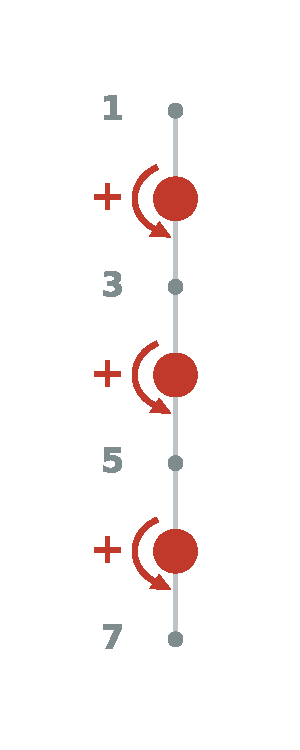
\includegraphics[scale=0.4]{diagram_chain_same_chir.pdf}
    \end{figure} 
        \end{column}
        \begin{column}{0.8\textwidth}
              \begin{figure}
        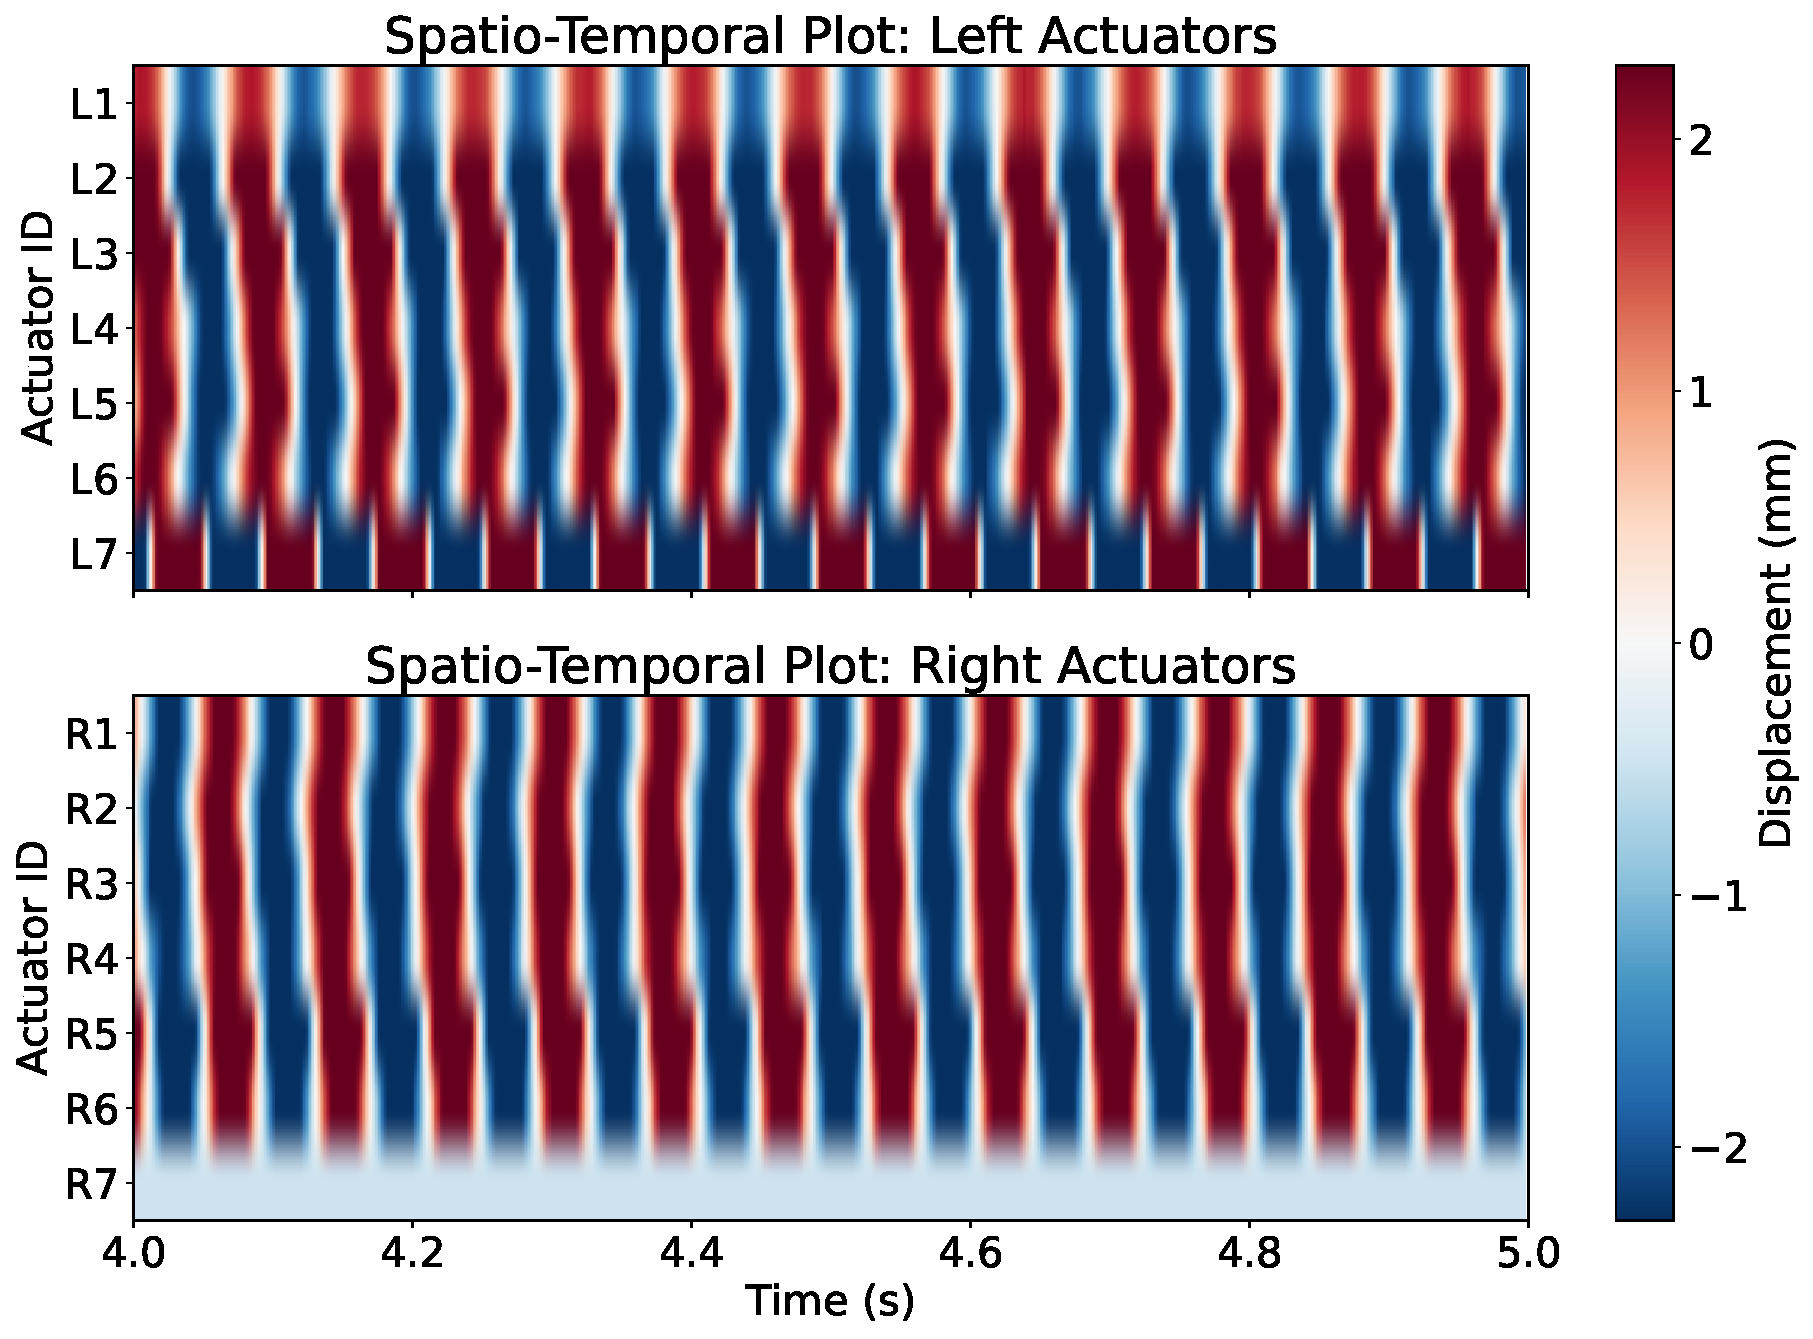
\includegraphics[width=\textwidth]{chain_same_chir.pdf}
    \end{figure}  
    \end{column}
    \end{columns}
         Synchronization instead of wave propagation due to autonomous oscillators
\end{frame}

\begin{frame}[allowframebreaks]{1d chain with opposite chirality attenuates}
    \begin{columns}
        \begin{column}{0.2\textwidth}
               \begin{figure}
        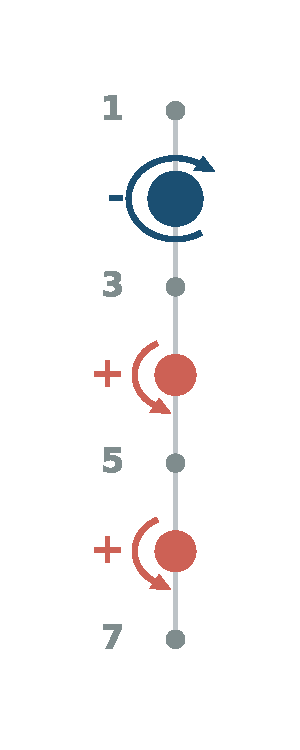
\includegraphics[scale=0.4]{diagram_chain_opp_chir_2.pdf}
    \end{figure} 
        \end{column}
        \begin{column}{0.8\textwidth}
              \begin{figure}
        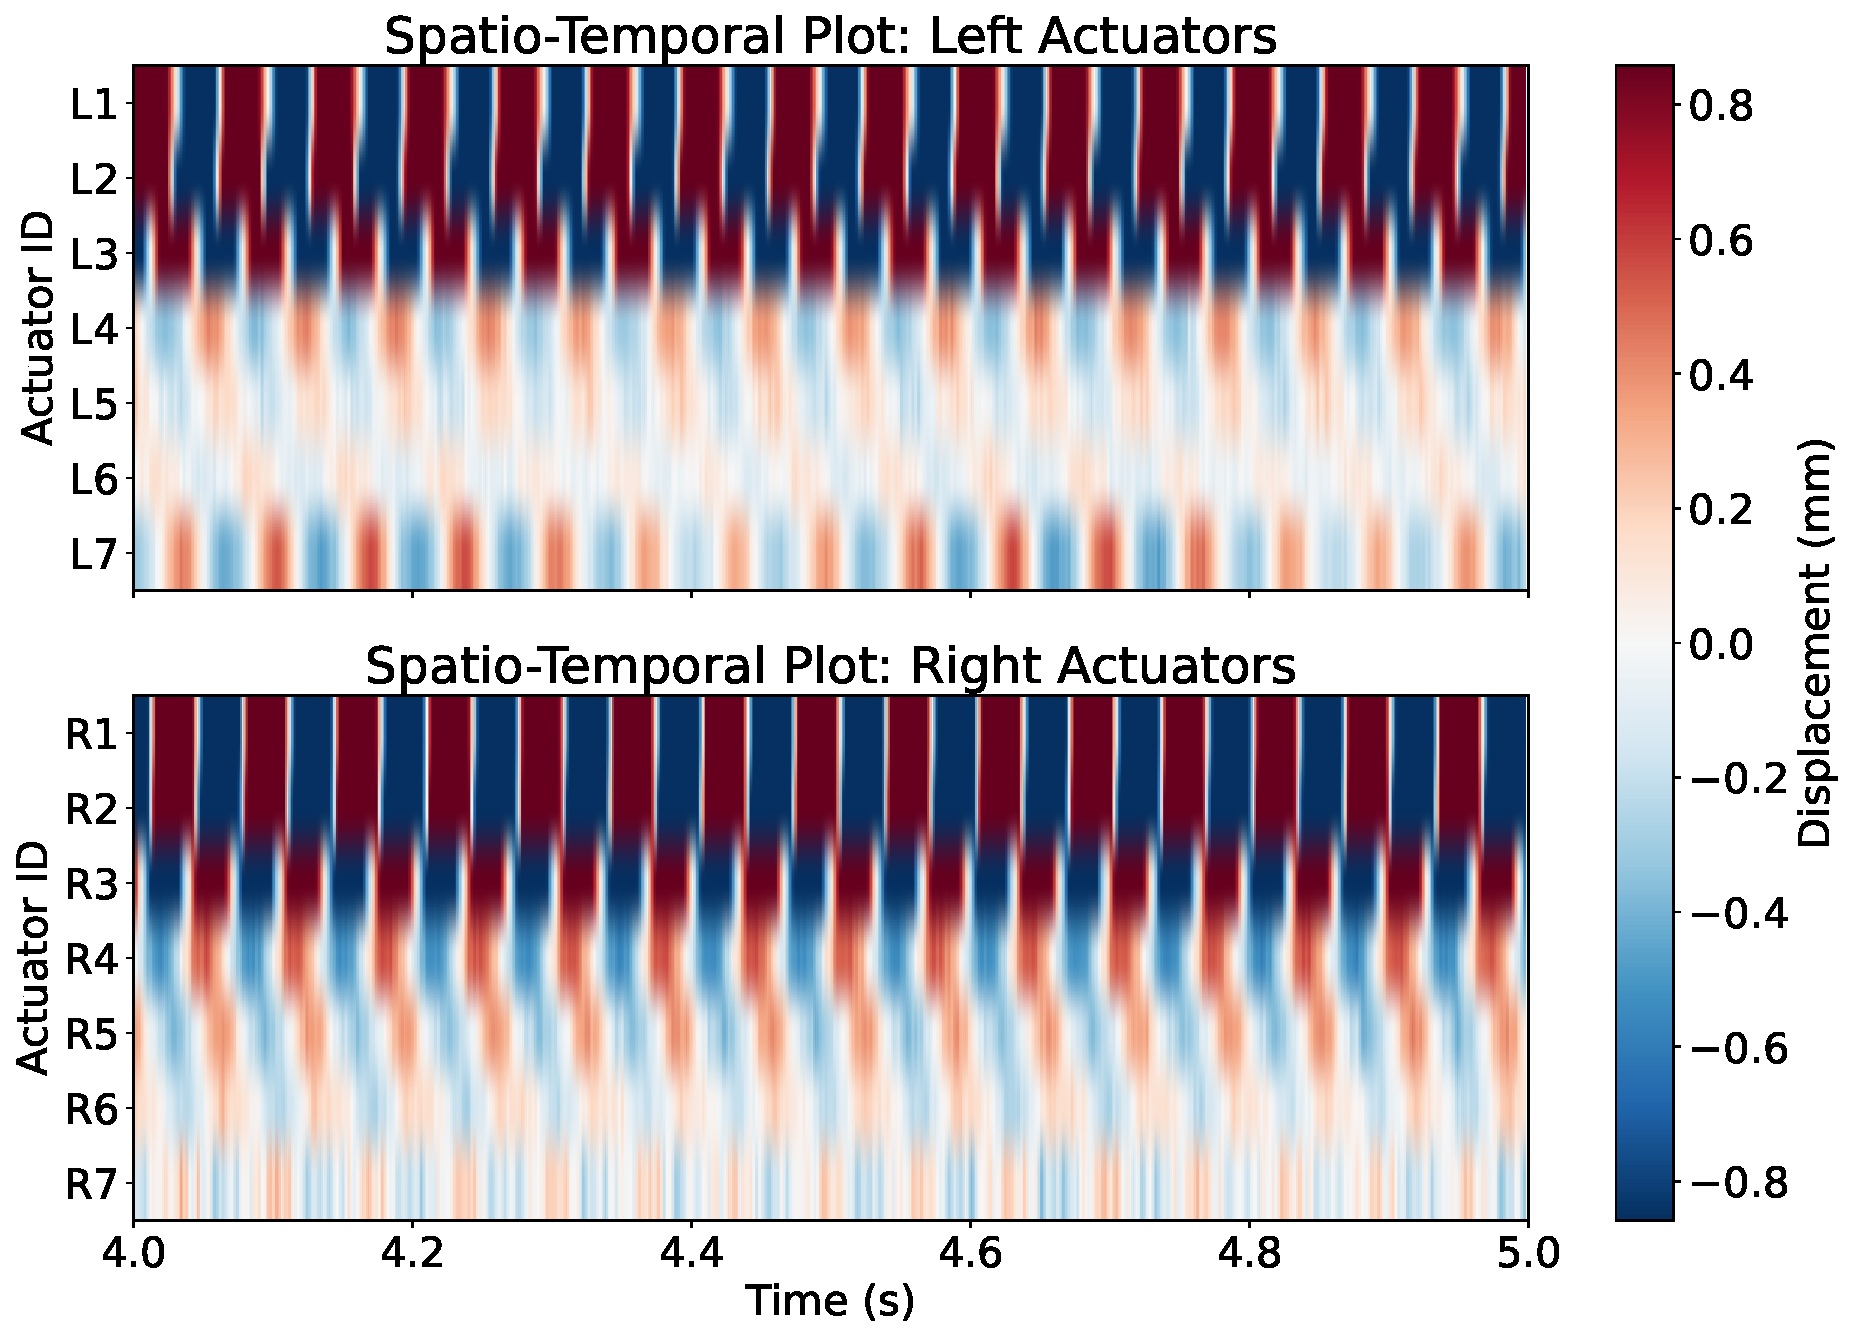
\includegraphics[width=\textwidth]{chain_opp_chir_2.pdf}
    \end{figure}  
    \end{column}
    \end{columns}
    Oscillation amplitude is significantly reduced
    \framebreak
    \begin{columns}
        \begin{column}{0.2\textwidth}
               \begin{figure}
        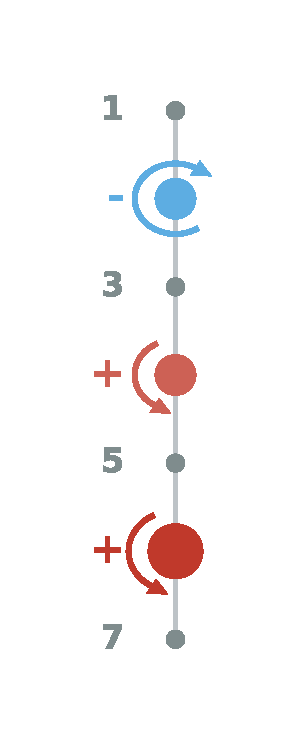
\includegraphics[scale=0.4]{diagram_chain_opp_chir_6.pdf}
    \end{figure} 
        \end{column}
        \begin{column}{0.8\textwidth}  
        \begin{figure}
        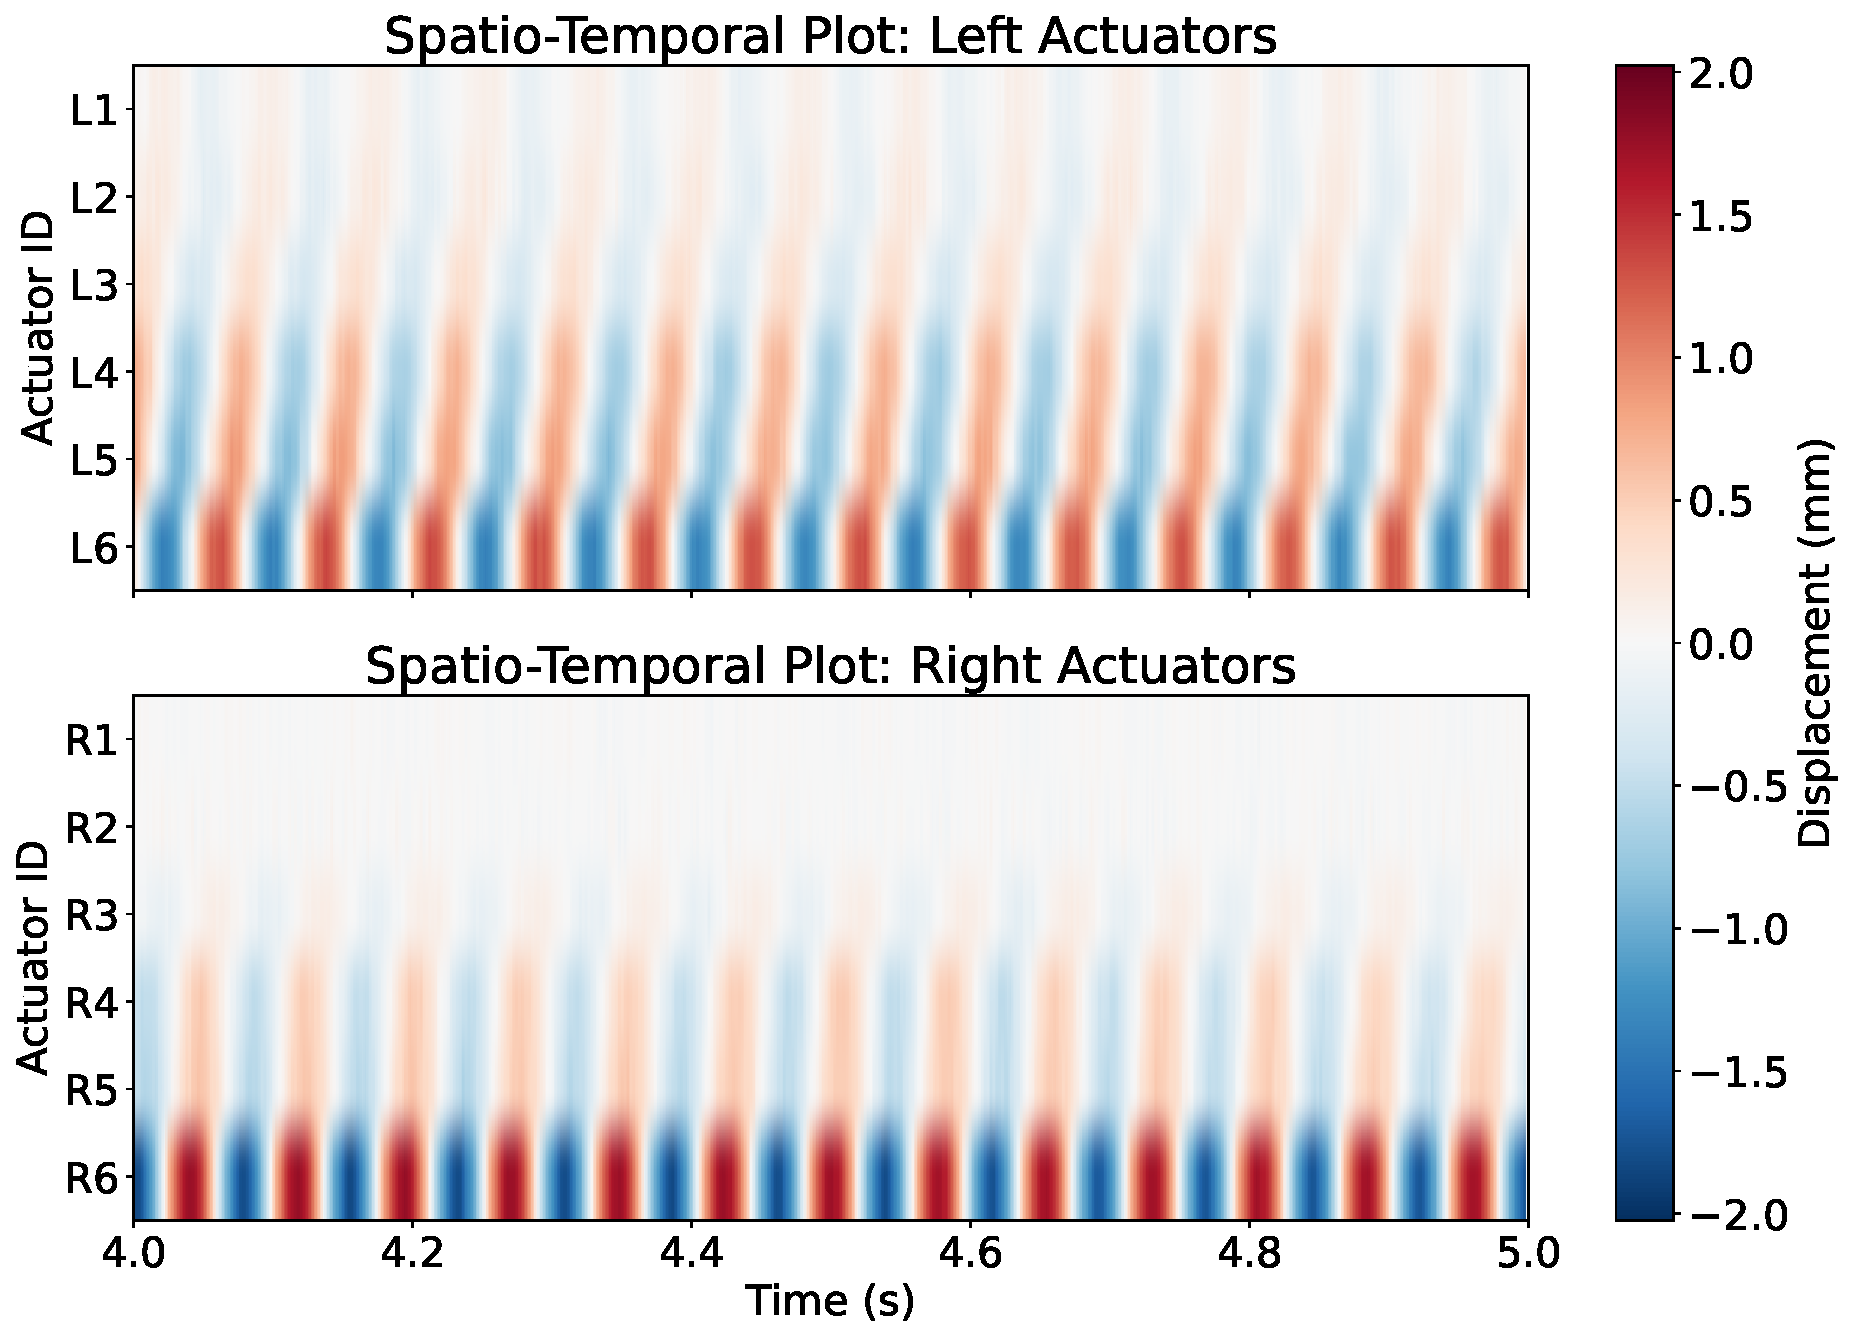
\includegraphics[width=0.9\textwidth]{chain_opp_chir_6.pdf}
    \end{figure}
    \end{column}
    \end{columns}
       Spin-momentum locking
\end{frame}

\begin{frame}{Long chain exhibits wave coarsening}
    \begin{figure}
        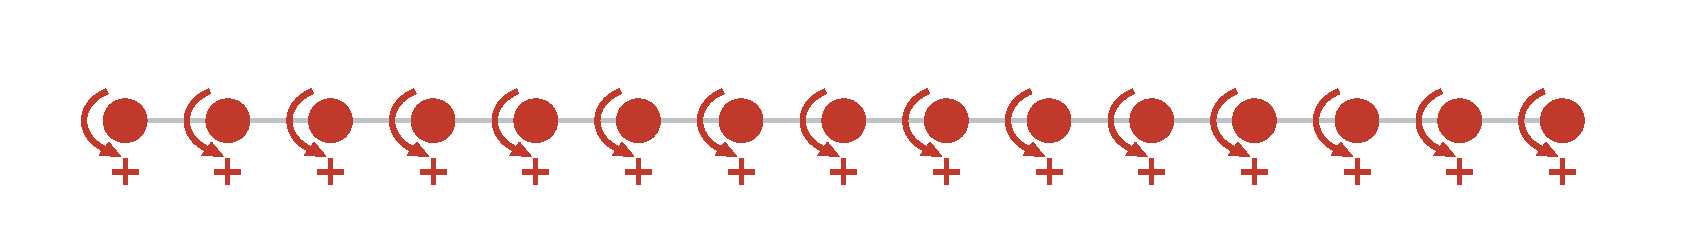
\includegraphics[width=\textwidth]{diagram_long_chain_wave_coarse.pdf}
    \end{figure}
    \begin{figure}
        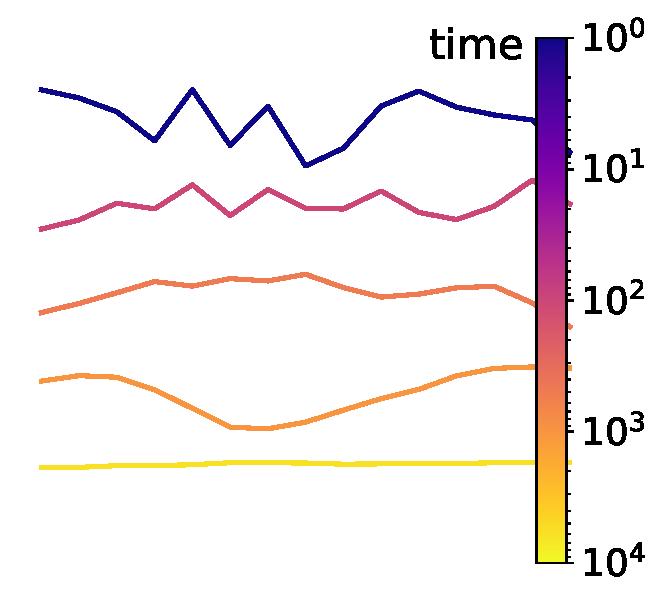
\includegraphics[width=0.5\textwidth]{chain_wave_coarsening.pdf}
    \end{figure}
    Simulation of 15 units
\end{frame}

\section{Lieb lattice}

\begin{frame}{Frustration in cross cell}
    \begin{columns}
        \begin{column}{0.5\textwidth}
        \begin{figure}
        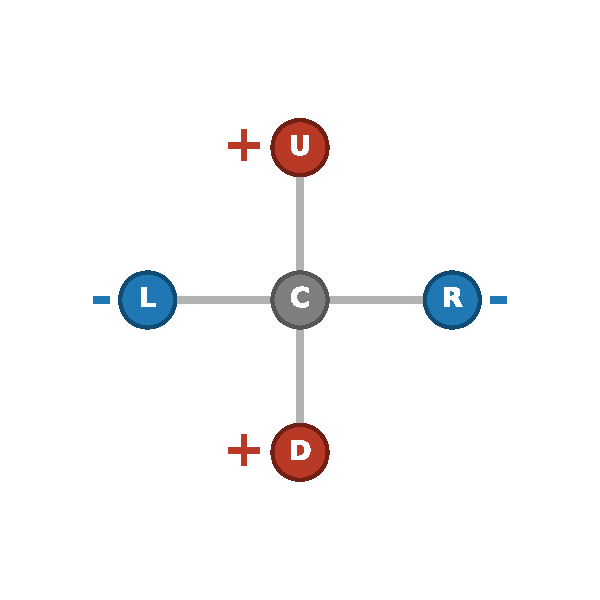
\includegraphics[scale=0.3]{diagram_am_cross_cell.pdf}
    \end{figure}
        \end{column}
        \begin{column}{0.5\textwidth}
            The passive center unit is bistable
        \end{column}
    \end{columns}

    \begin{figure}
        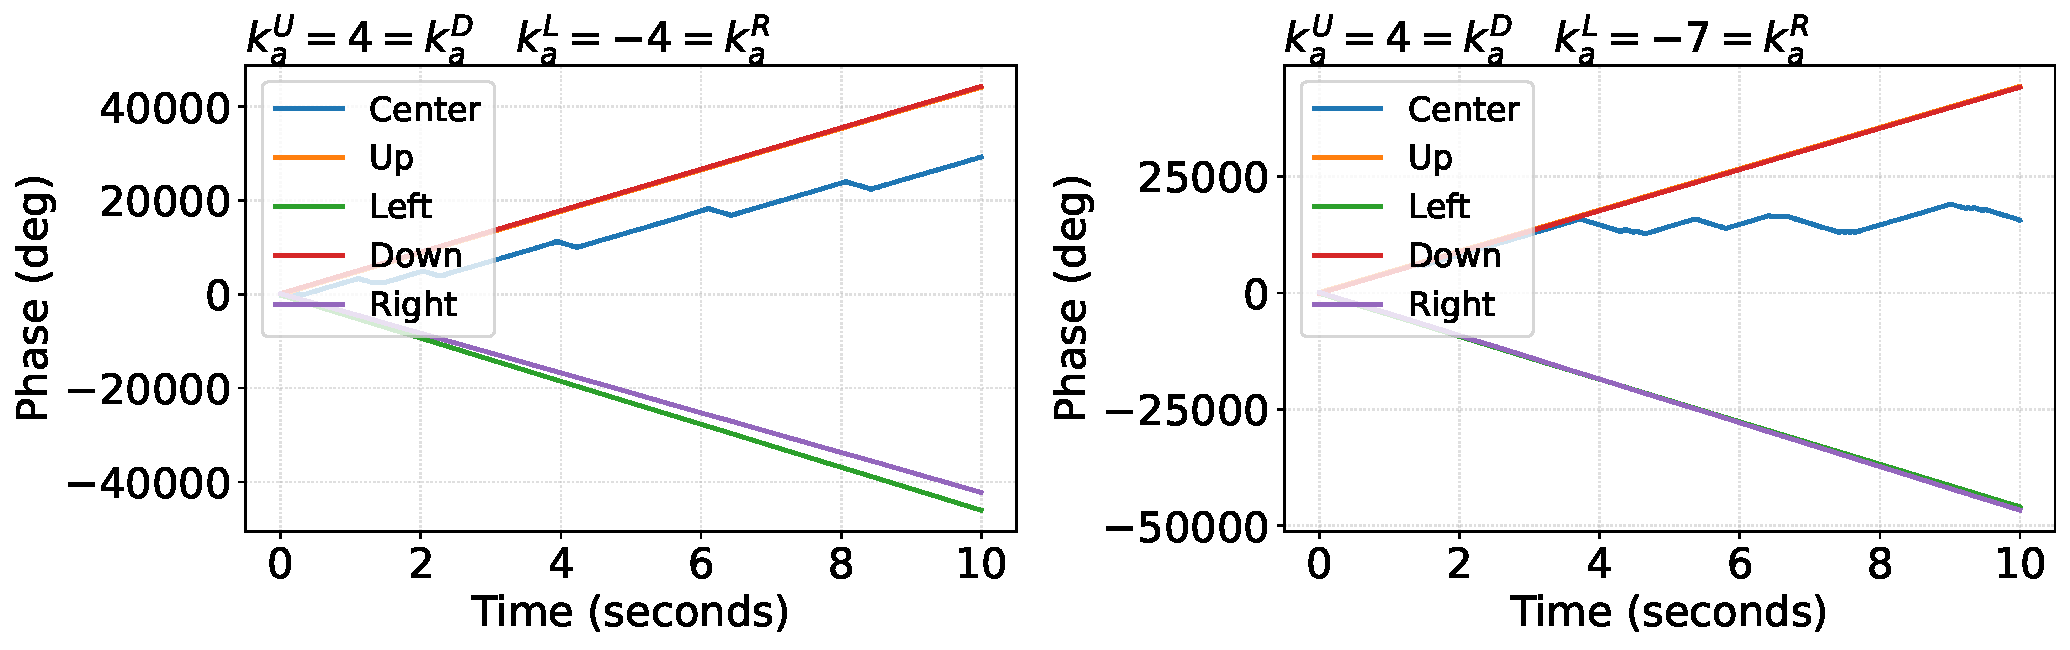
\includegraphics[width=\textwidth]{cross_cell_phase.pdf}
    \end{figure}
\end{frame}

% \begin{frame}{Rupesh's continuum model}
% \begin{equation}
%     R_s(t) = x_{1,s}(t) + i\, x_{2,s}(t).
%     \label{eq:complex-R}
% \end{equation}
%     \begin{equation}
%     \ddot{R}_s
%     = -\Gamma \dot{R}_s
%       - k_0 R_s
%       + i\,k_a \sigma_s\, R_s
%       - k_c \left[ (\Re R_s)^3 + i\,(\Im R_s)^3 
%       - k_{\text{link}} \sum_{s' \in \mathcal{N}(s)} (R_s - R_{s'})\right].
%     \label{eq:R-full}
% \end{equation}
% \end{frame}

\begin{frame}{Mechanical Lieb lattice}

        Below Hopf bifurcation: spin-momentum locking
    \vfill
    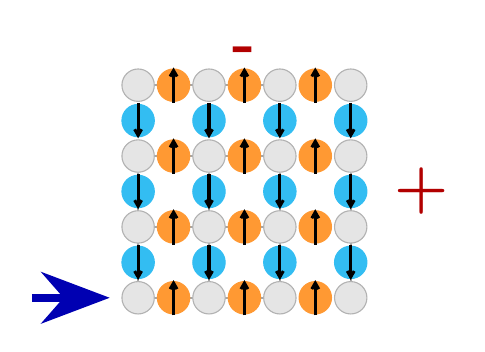
\begin{tikzpicture}[
    scale=0.9, transform shape,
    % Node styles
    siteB/.style={circle, draw=gray!60, fill=gray!20, minimum size=13pt, inner sep=0pt},
    siteA/.style={circle, draw=orange!80, fill=orange!80, minimum size=13pt, inner sep=0pt},
    siteC/.style={circle, draw=cyan!80, fill=cyan!80, minimum size=13pt, inner sep=0pt},
    % Big operators
    bigarrow/.style={line width=3pt, -{Stealth[scale=1.5]}, draw=blue!70!black},
    % Spin arrows: Longer (from 0.18 to 0.25), open diagonal bars, completely unfilled
    spinarrow/.style={line width=1.1pt, -{Straight Barb[angle=60:2.5pt, open]}, draw=black}
]

    % =========================================================================
    % 1. LEFT SIDE: BIG ARROW
    % =========================================================================
    \draw[bigarrow] (-1.5, 0) -- (-0.4, 0);

    % =========================================================================
    % 2. CENTER: 3x3 LIEB LATTICE 
    % =========================================================================
    
    % --- Lattice Grid Lines (Bonds) ---
    \foreach \x in {0, 1, 2, 3} {
        \draw[dashed, line width=0.6pt, gray!70] (\x, 0) -- (\x, 3);
        \draw[dashed, line width=0.6pt, gray!70] (0, \x) -- (3, \x);
    }

    % --- Generation Loops ---
    \foreach \x in {0,...,3} {
        \foreach \y in {0,...,3} {
            
            % 1. Neutral B-sites
            \node[siteB] at (\x, \y) {};
            
            % 2. A-sites (Horizontal, up-spins)
            \ifnum \x < 3
                \node[siteA] at (\x+0.5, \y) {}; 
                % Lengthened span to make the spin-arrow more prominent
                \draw[spinarrow] (\x+0.5, \y-0.25) -- (\x+0.5, \y+0.25);
            \fi
            
            % 3. C-sites (Vertical, down-spins)
            \ifnum \y < 3
                \node[siteC] at (\x, \y+0.5) {}; 
                % Lengthened span to make the spin-arrow more prominent
                \draw[spinarrow] (\x, \y+0.75) -- (\x, \y+0.25);
            \fi
        }
    }

    % =========================================================================
    % 3. RIGHT SIDE: BIG PLUS SIGN
    % =========================================================================
    \node[text=red!70!black] at (4.0, 1.5) {\fontsize{30}{30}\selectfont \textbf{+}};
    \node[text=red!70!black] at (1.5, 3.5) {\fontsize{40}{40}\selectfont \textbf{-}};

\end{tikzpicture}
\hfill
\uncover<2->{
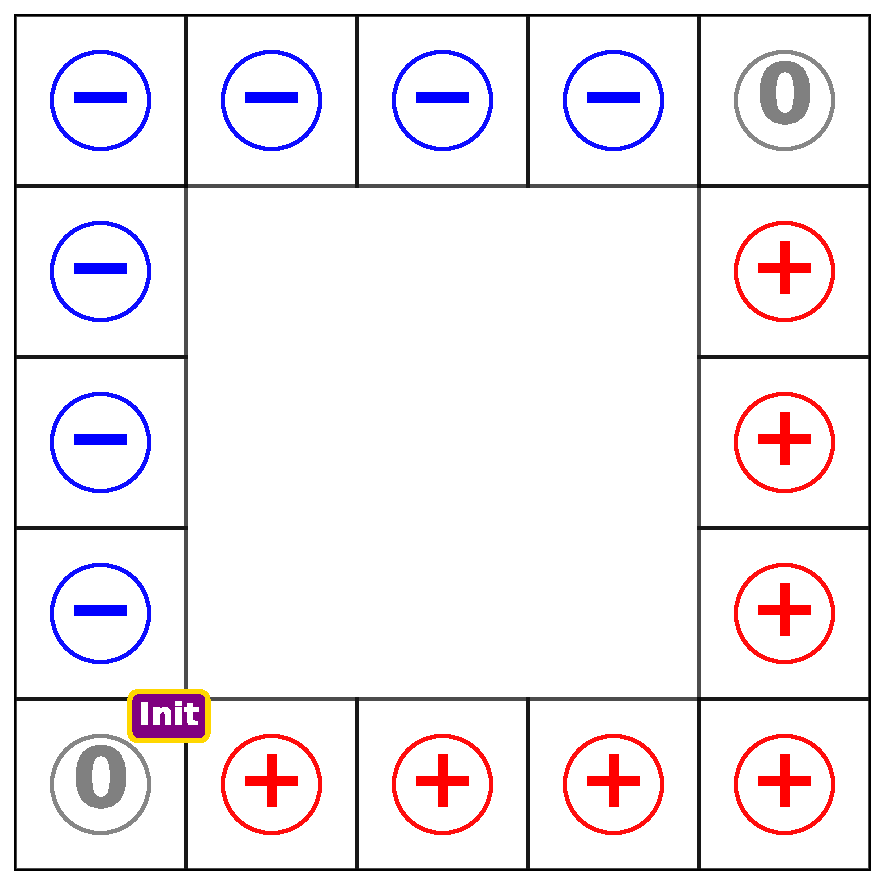
\includegraphics[width=0.4\textwidth]{lieb_sml_gen_compacted.pdf}
\vfill
Chirality measured as the sign of $J=\xd_1x_2-x_1\xd_2$
}
\end{frame}

\begin{frame}{Chirality in mechanical Lieb lattice}
    \begin{columns}
    \begin{column}{0.5\textwidth}
        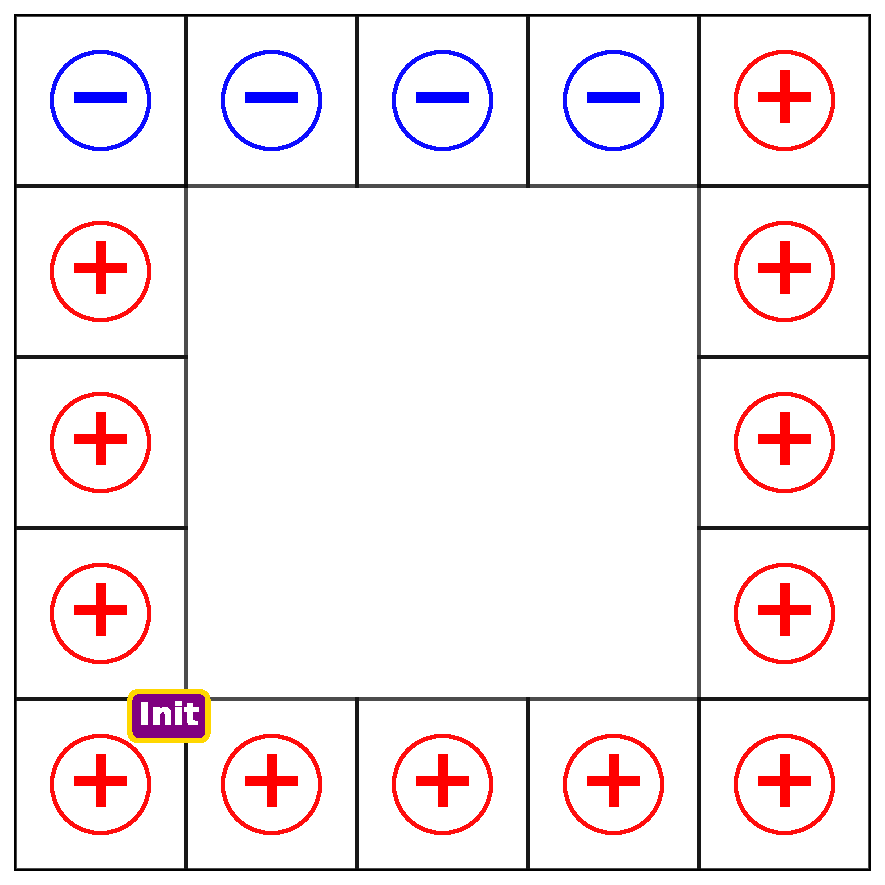
\includegraphics[width=\textwidth]{lieb_sml_pos_compacted.pdf}
    \end{column}
    \begin{column}{0.5\textwidth}
        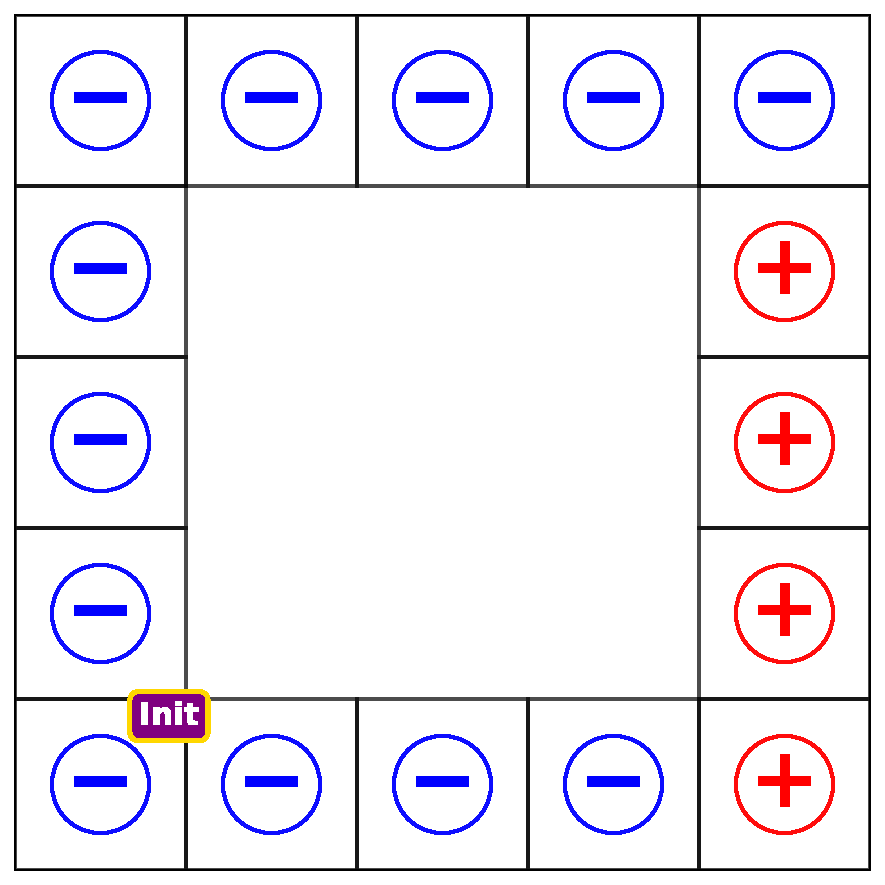
\includegraphics[width=\textwidth]{lieb_sml_neg_compacted.pdf}
    \end{column}
    \end{columns}
    \vfill
    Chirality measured as the sign of $J=\xd_1x_2-x_1\xd_2$
\end{frame}

\section{Conclusions}

\begin{frame}{Conclusions}
    \begin{itemize}
        \setlength{\itemsep}{\baselineskip}
        \item Implemented "mechanical spin" \pause 
        \item Built a mechanical altermagnet  \pause 
    \end{itemize}
    \vfill
    \begin{alertblock}{Main conclusion}
        Spin-momentum locking $\longrightarrow$ selective propagation in different directions
    \end{alertblock}
\end{frame}

\begin{frame}{Acknowledgements}
    % === TOP ROW: 3 Supervisors ===
    \begin{columns}[t]
        \begin{column}{.23\textwidth}
            \centering
            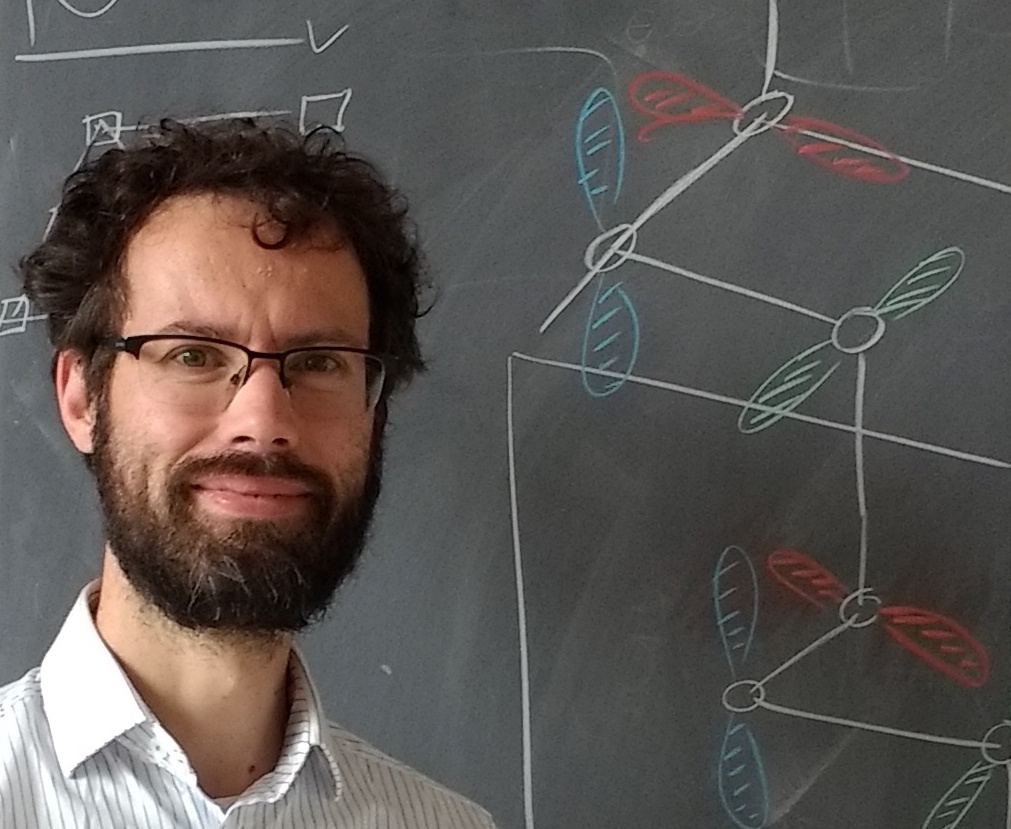
\includegraphics[height=2.2cm]{Jasper1.jpg}\\
            \small Jasper van Wezel
        \end{column}
        
        \begin{column}{.23\textwidth}
            \centering
            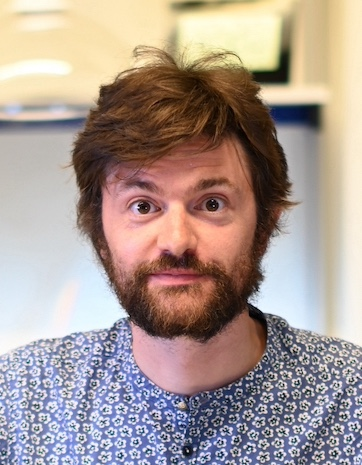
\includegraphics[height=2.2cm]{corentin.jpg}\\
            \small Corentin Coulais
        \end{column}

        \begin{column}{.23\textwidth}
            \centering
            
\includegraphics[height=2.2cm]{ronald_image.png}\\ 
            \small Ronald Hassing 
        \end{column}

    \begin{column}{.23\textwidth}
            \centering
            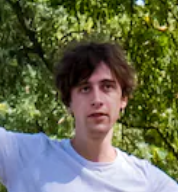
\includegraphics[height=2.2cm]{kasper_image.PNG}\\
            \small Kasper van Nieuwland
        \end{column}
        \end{columns}
    
    \vspace{0.4cm} % Adjusts the gap between the top and bottom rows
    
    % === BOTTOM ROW: 4 Supervisors ===
    \begin{columns}[t]
        \begin{column}{.23\textwidth}
            \centering
            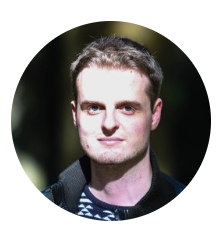
\includegraphics[height=2.2cm]{viktor.png}\\
            \small Viktor Könye
        \end{column}
        
        \begin{column}{.23\textwidth}
            \centering
            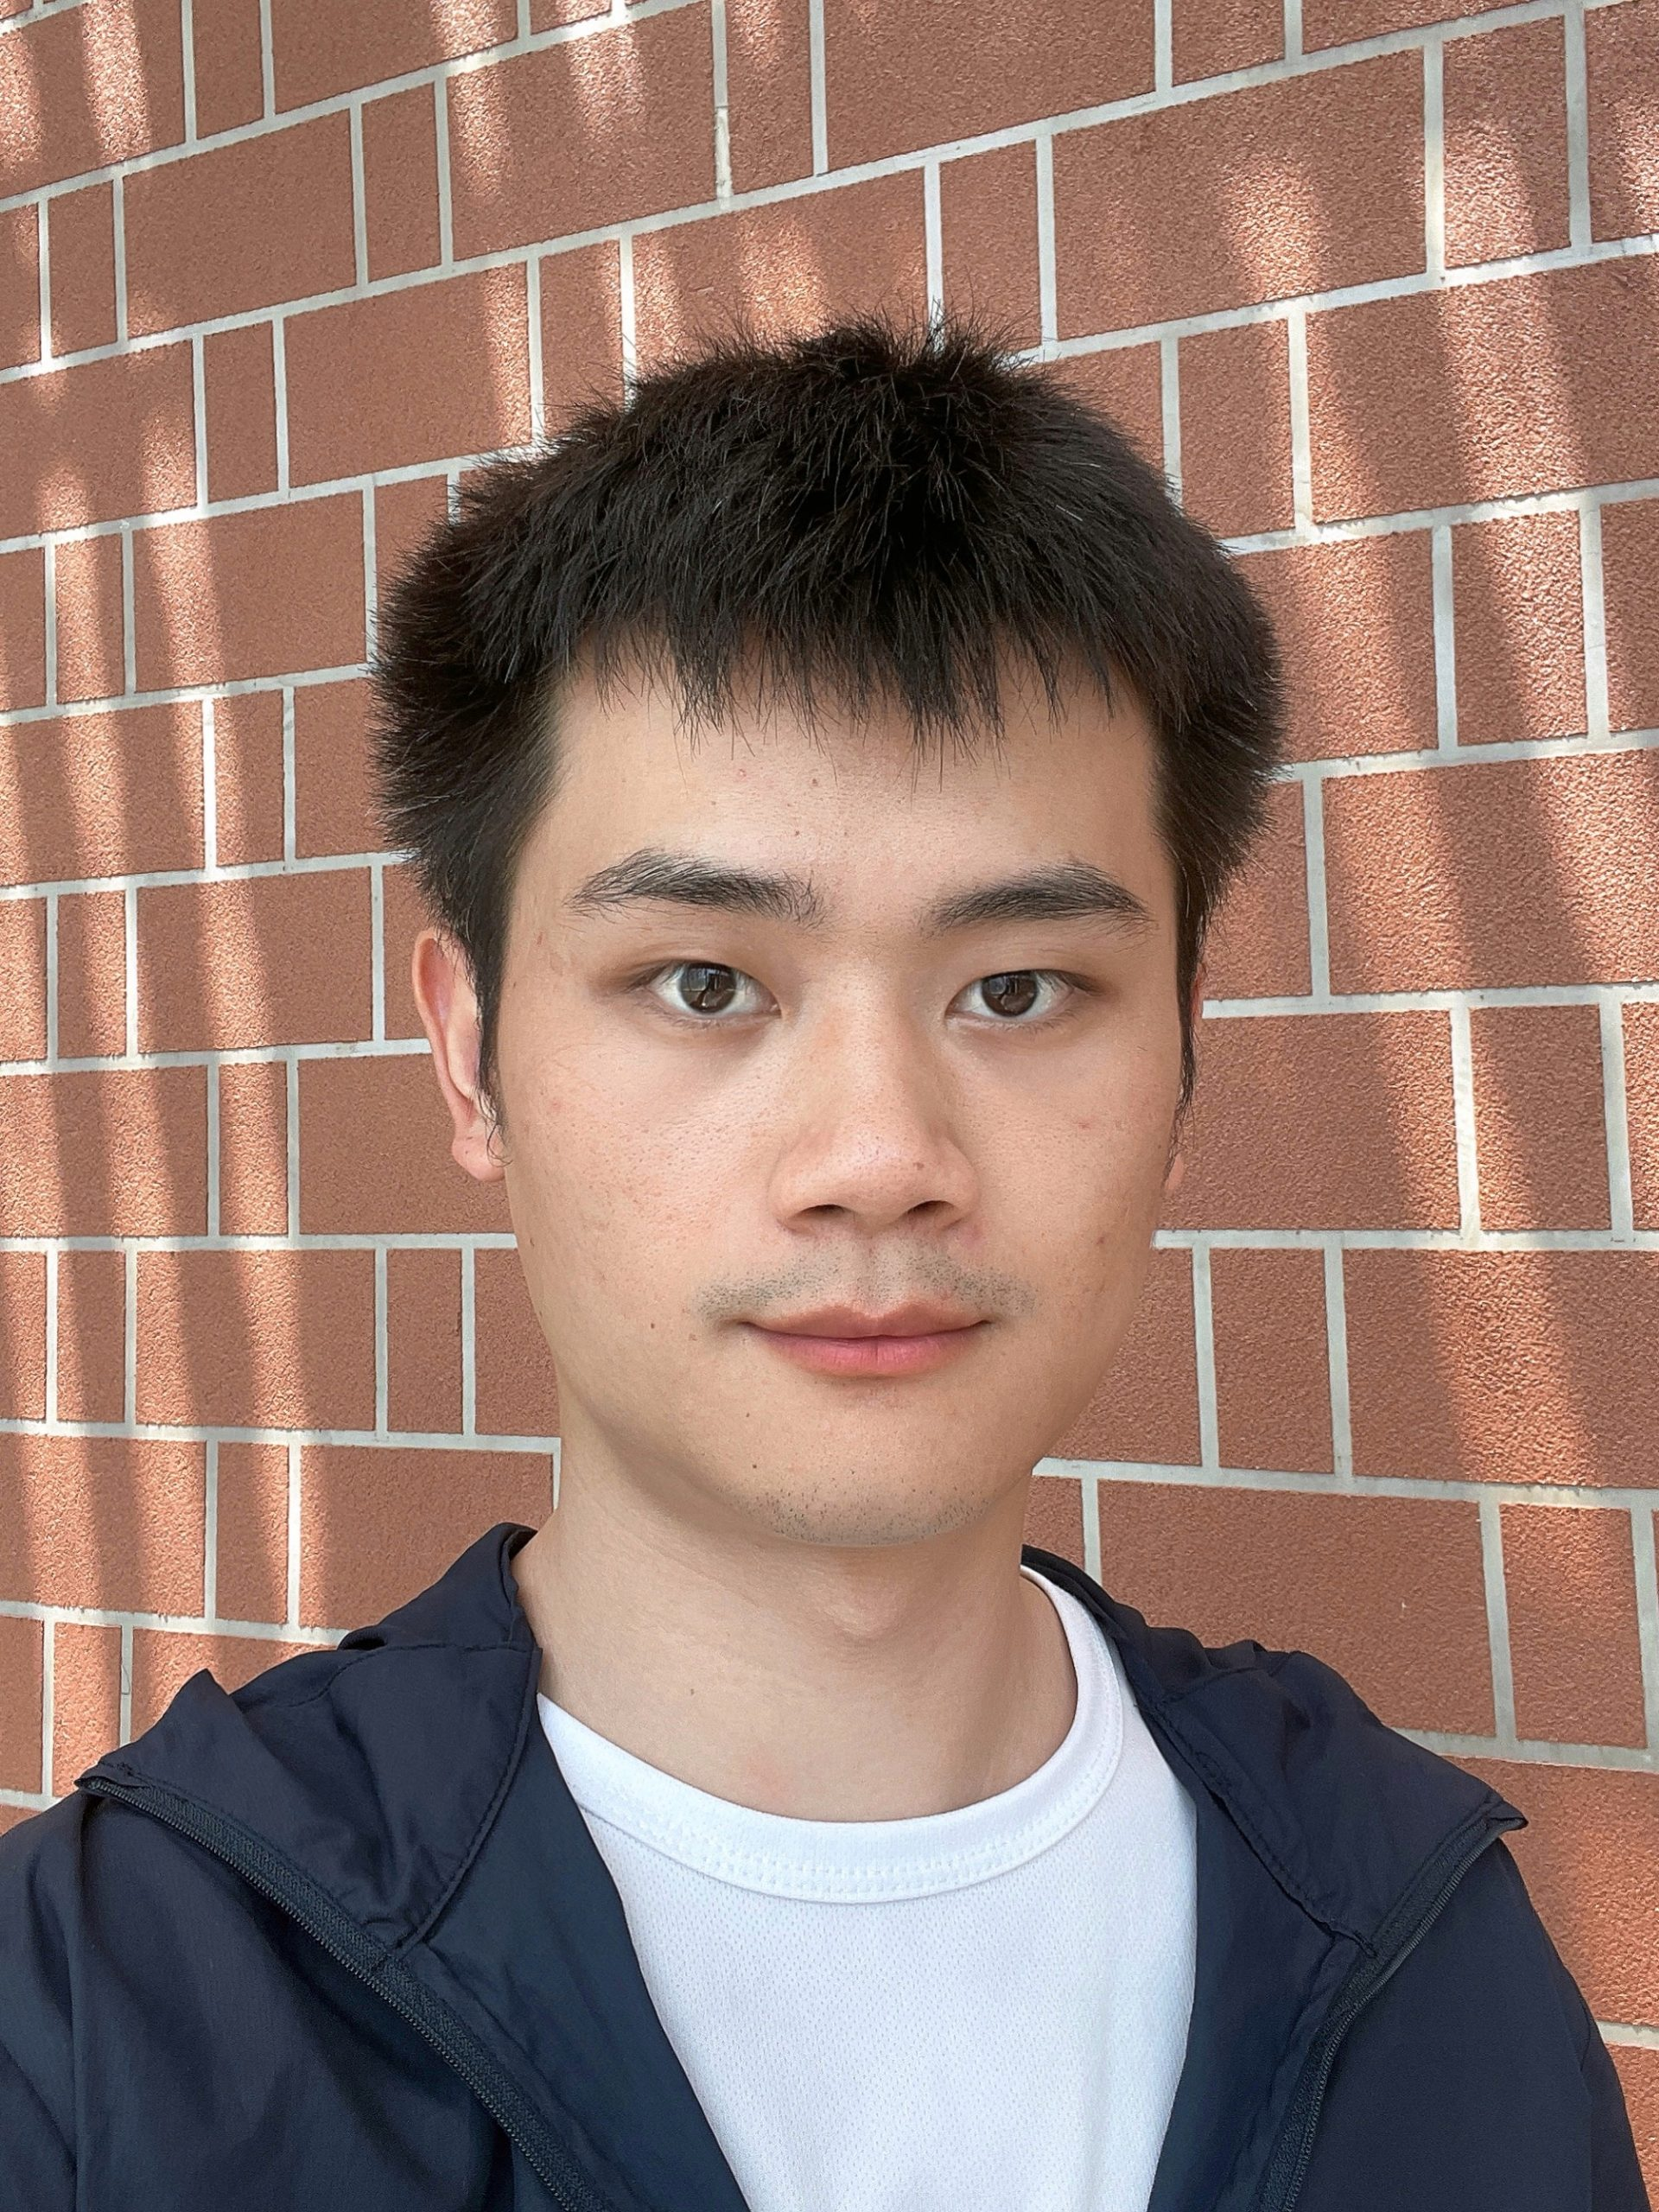
\includegraphics[height=2.2cm]{yuan.jpeg}\\
            \small Yuan Zhou
        \end{column}
        
        \begin{column}{.23\textwidth}
            \centering
            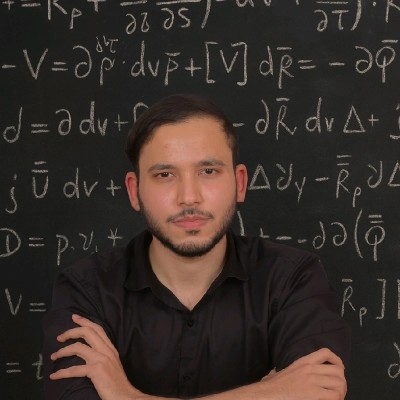
\includegraphics[height=2.2cm]{rupesh_image.png}\\
            \small Rupesh Mahore
        \end{column}

        \begin{column}{.23\textwidth}
            \centering
            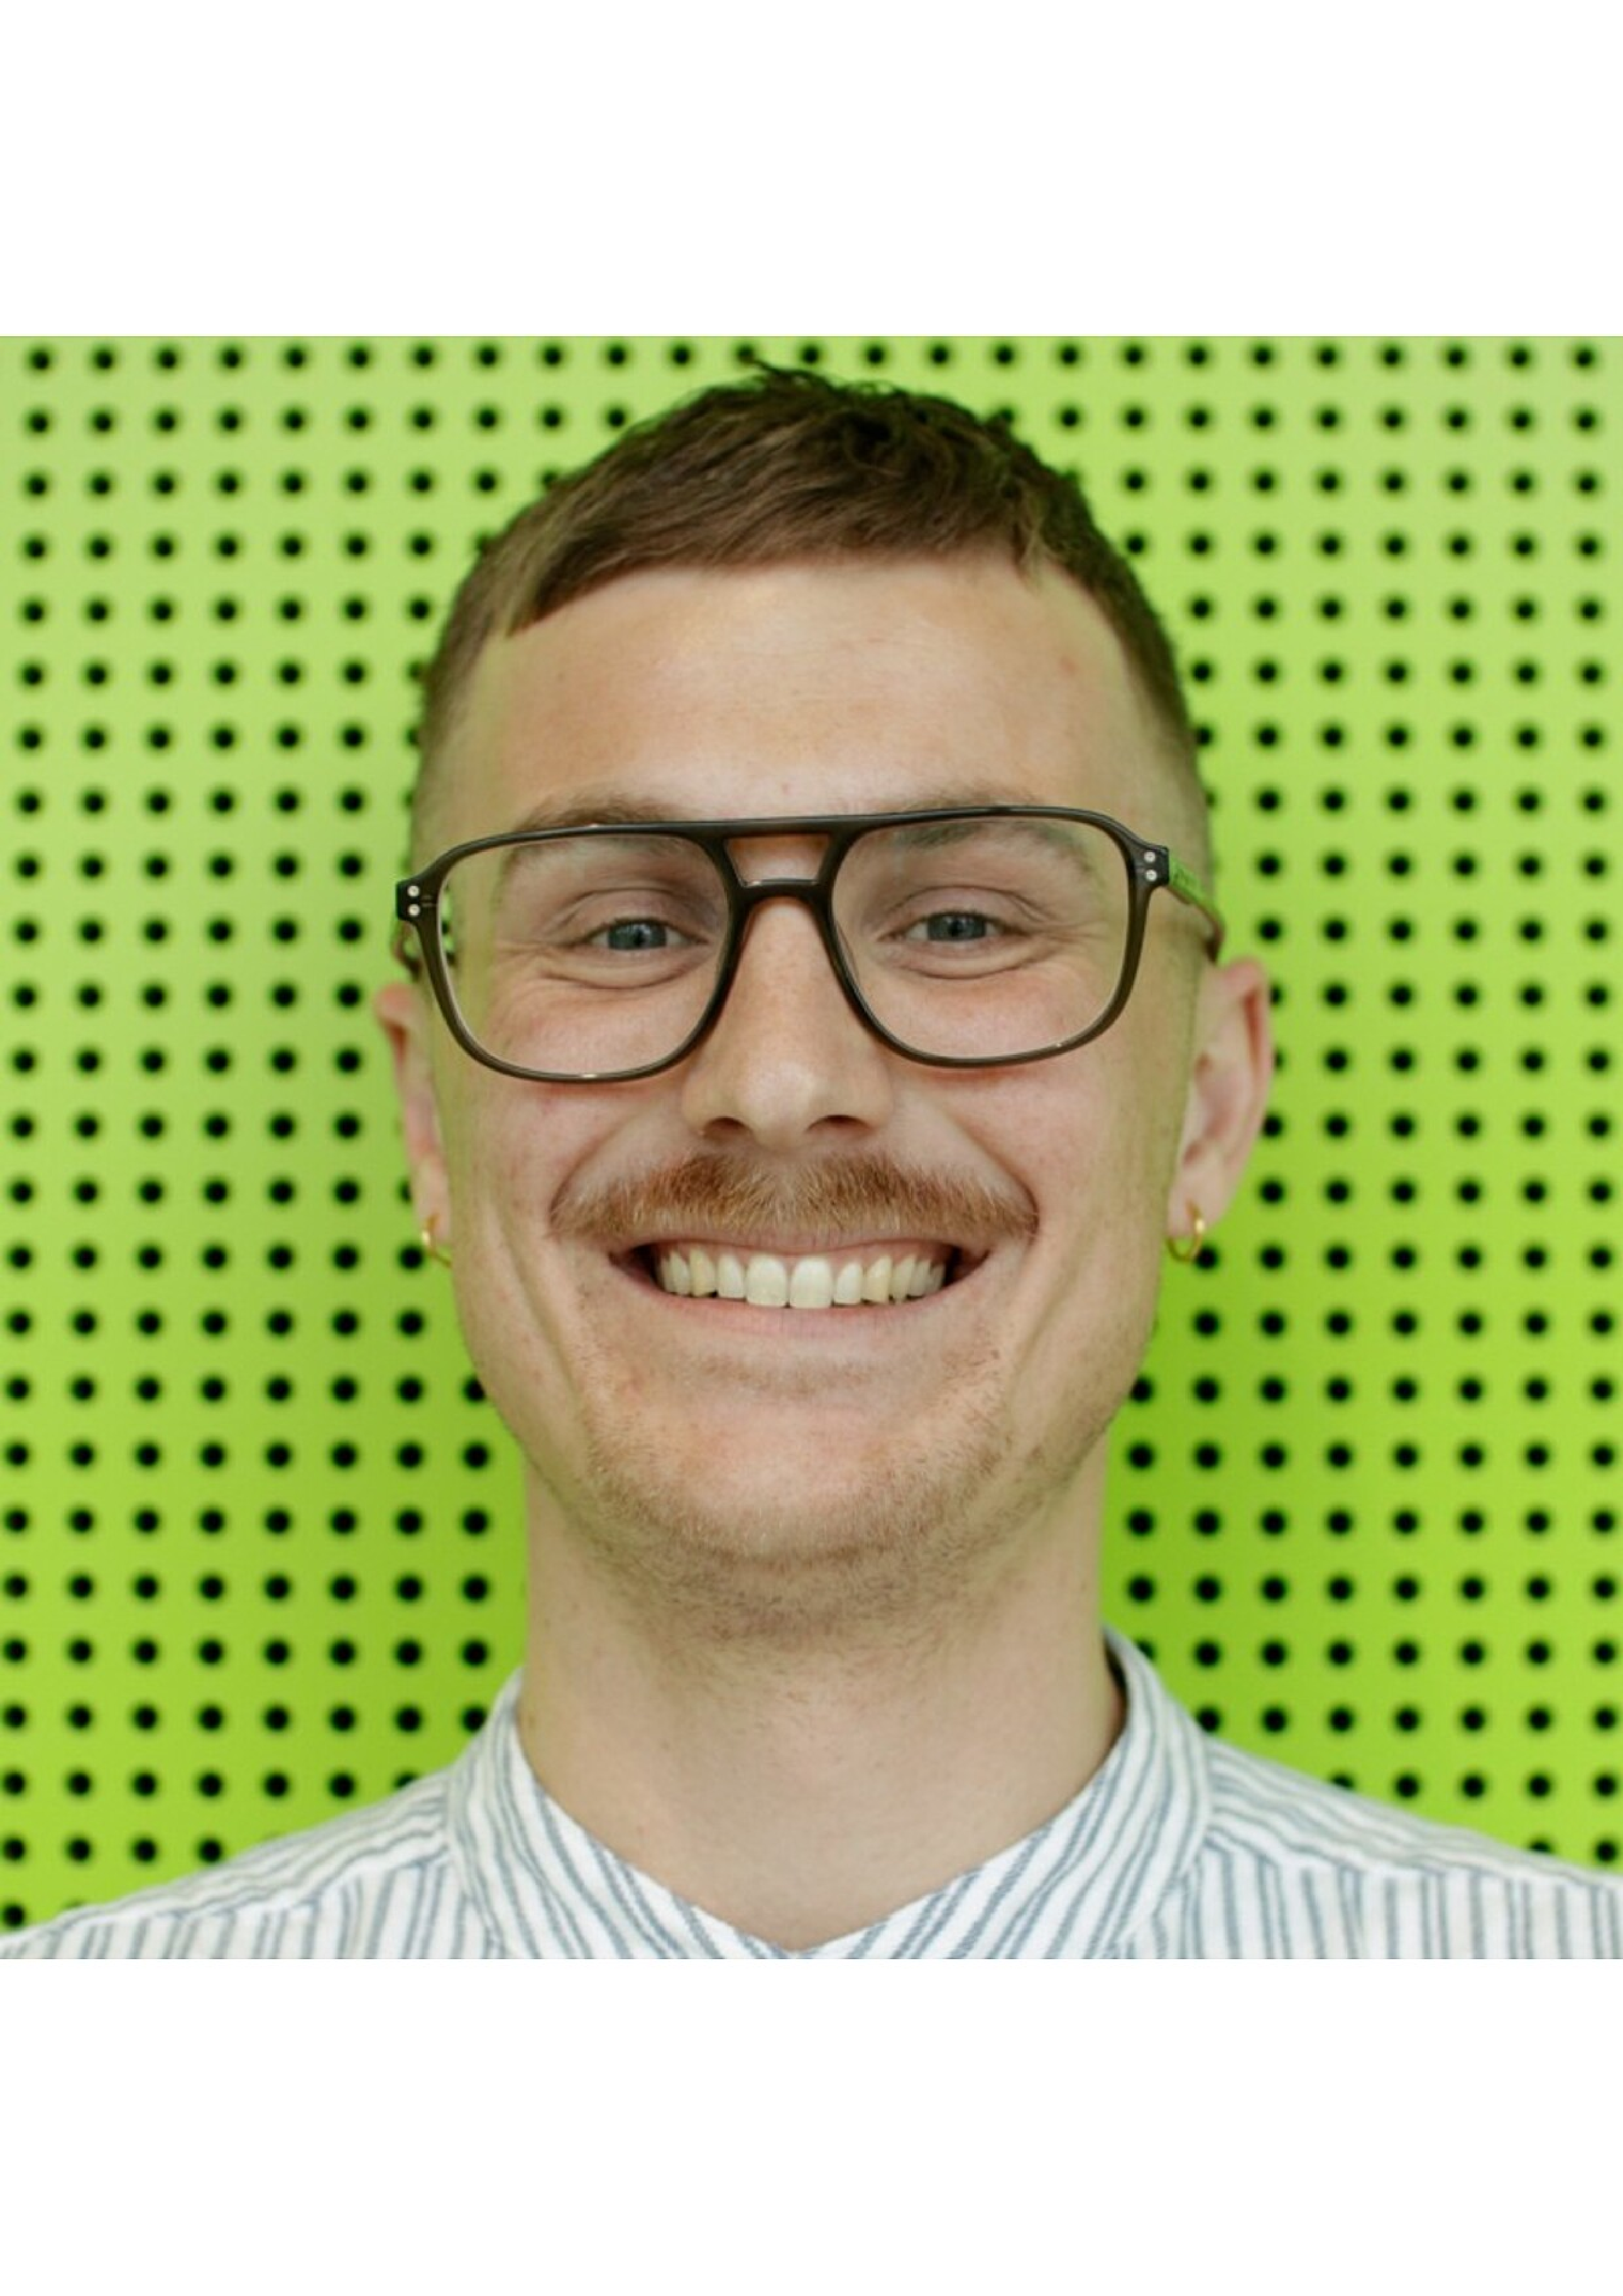
\includegraphics[height=2.2cm]{image_mels.pdf}\\
            \small Mels van Eck 
        \end{column}
    \end{columns}
\end{frame}



%\section{Annex}
 \appendix

% \section{Annex}

% \begin{frame}{Frequency of one unit}
%     \begin{figure}
%         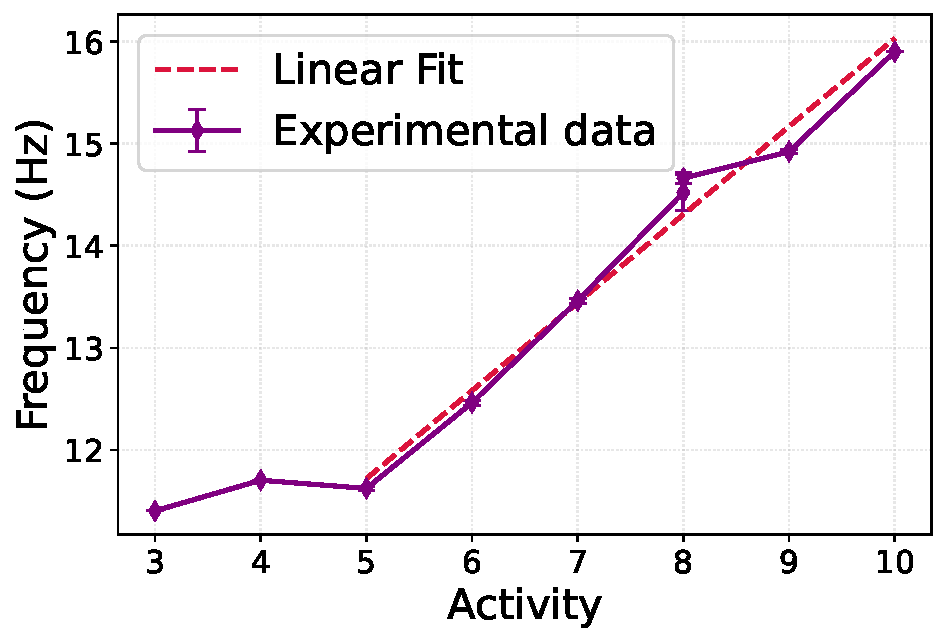
\includegraphics[width = \textwidth]{linear_frequency_scaling_one_node.pdf}
%     \end{figure}
%     Hopf bifurcation predicts linear dependence: $\omega = \frac{k_a}{\gamma}$
% \end{frame}

% \begin{frame}{Amplitude of one unit}
%     \begin{figure}
%         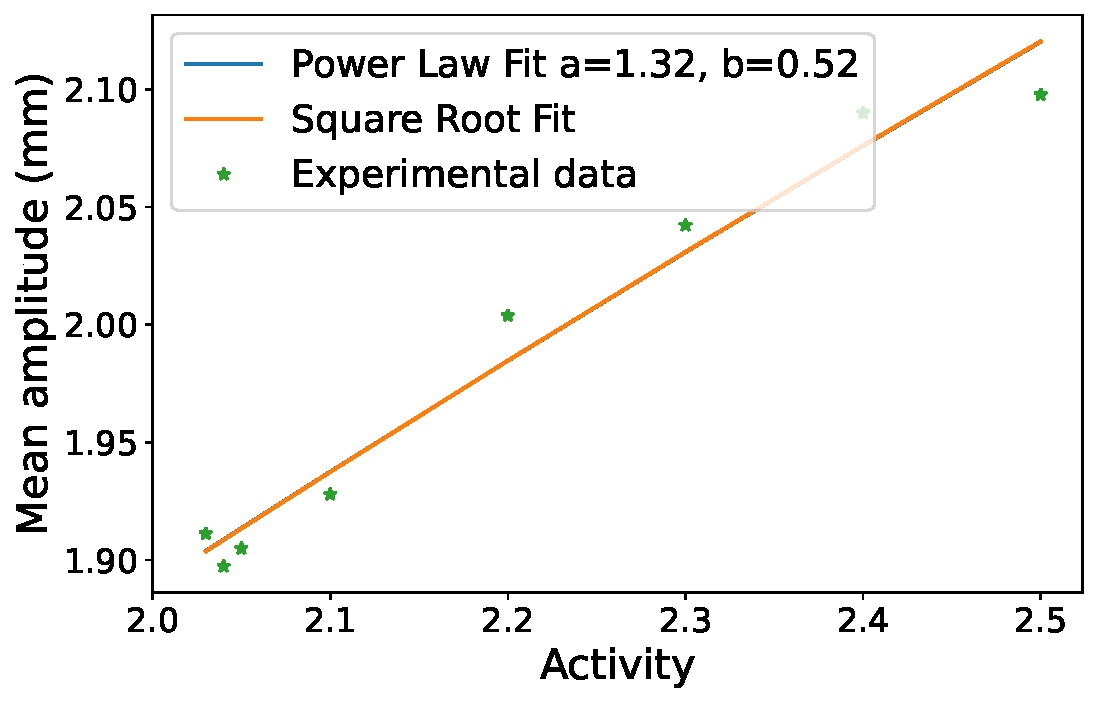
\includegraphics[width = 0.8\textwidth]{amplitude_scaling_Hopf.pdf}
%     \end{figure} 
%      Hopf bifurcation predicts $R \sim \sqrt{\frac{2k_a^c}{k_c\gamma^2}(k_a-k_a^c)}$
% \end{frame}

% \begin{frame}{Magnetism}
% \begin{itemize}
%     \item Magnets break time-reversal symmetry % or spin-rotational/
% %\vspace{-0.4em}
% \begin{center}
%     \begin{tikzpicture}
%     \node[anchor=south west, inner sep=0] (image) at (0,0) {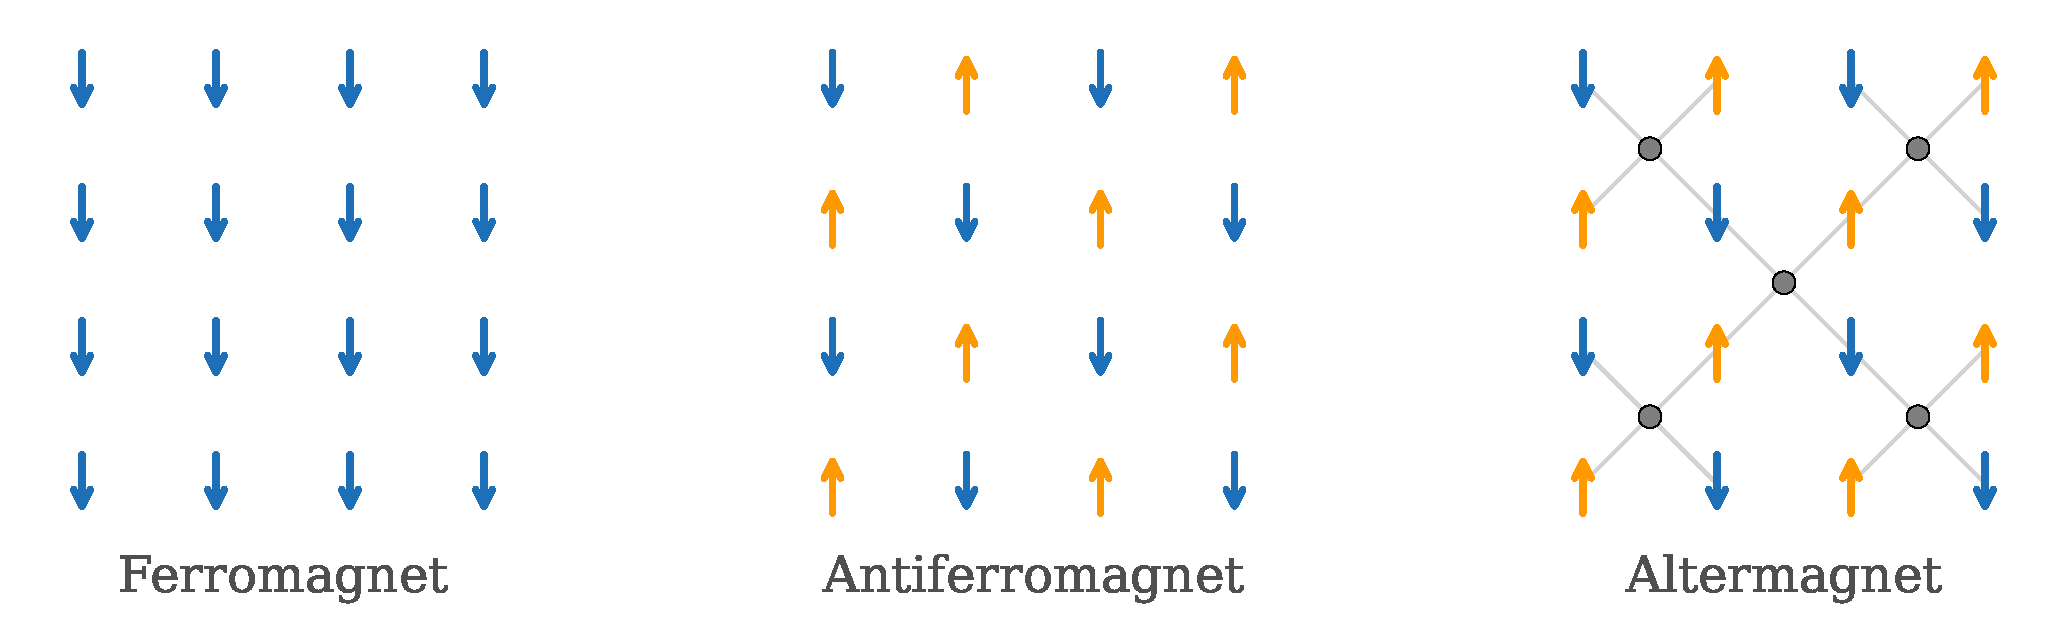
\includegraphics[width=0.9\textwidth]{magnetic_phases.pdf}};
%     \begin{scope}[x={(image.south east)},y={(image.north west)}]
%     \end{scope}
% \end{tikzpicture}
% \end{center}
% %\vspace{-0.5em}
%     \item Search for real space transformation that combined with time-reversal becomes a symmetry
%     \item Discovery of altermagnets in 2022 \cite{smejkal2022}
% \end{itemize}
% %\vspace{-0.4em}
%   \vfill % Empuja las citas al final de la diapositiva
  
%   \scalebox{0.6}{ % Reduce el tamaño visual general
%     \color{gray}
%     \begin{minipage}{1.5\textwidth} % Caja con ancho suficiente para el texto
%       \cite{smejkal2022} \fullcite{smejkal2022}
%     \end{minipage}
%   }
% \end{frame}

% \begin{frame}{Magnetism}
%     \begin{figure}
%         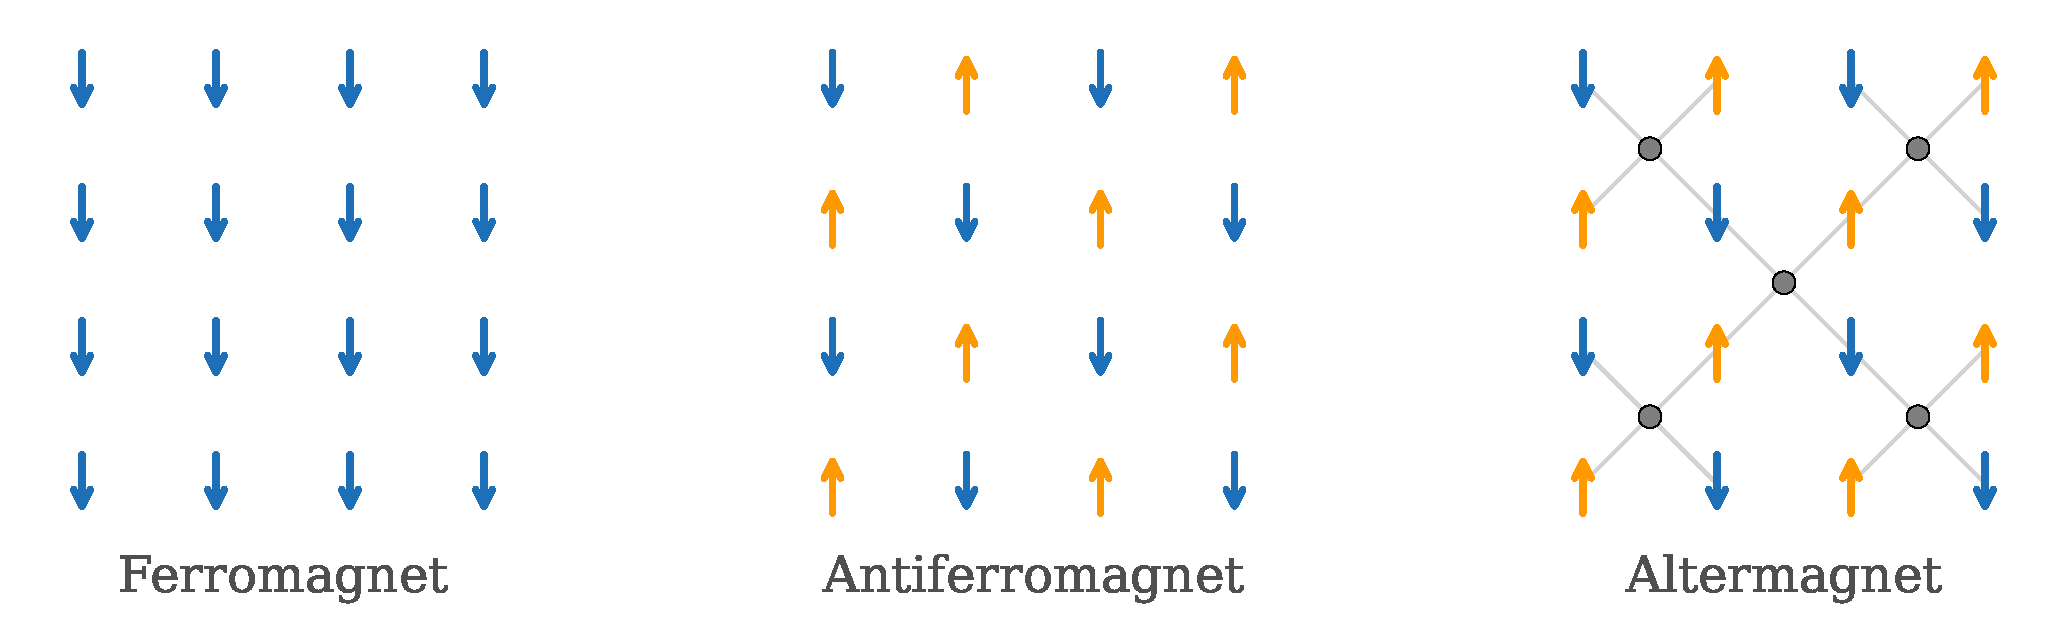
\includegraphics[width = 0.8\textwidth]{magnetic_phases.pdf}
%         \caption{a}
%     \end{figure} 
%     %Kramer's theorem: TRS + half-integer spin $\Longrightarrow$ degenerate energies
% \end{frame}

% \begin{frame}
%     \begin{tikzpicture}[scale=2]
%     % Define background/containment circle to keep things clean
%     \draw[thick] (0,0) circle (2cm);
    
%     % Clip everything inside the main radius to ensure sharp outer edges
%     \clip (0,0) circle (2cm);
%     % Render the 4 alternating lobes (rotated by 90 degrees each)
%     \yinyanglobe{0}{black}{white}
%     \yinyanglobe{90}{white}{black}
%     \yinyanglobe{180}{black}{white}
%     \yinyanglobe{270}{white}{black}
    
%     % Re-draw the clean outer boundary line over the shapes
%     \draw[thick] (0,0) circle (2cm);
    
% \end{tikzpicture}
% \end{frame}

% \begin{frame}{What are altermagnets? A different phase of matter}
%     \begin{enumerate}
%         \item Symmetry: Rotation+TR  denoted by $C_4\mathcal{T} $
%         \item Zero magnetization  
%         \item Spin-split bands
%         \item $C_4\mathcal{T} \Longrightarrow N_\uparrow = N_\downarrow$
%     \end{enumerate} 
%     % include table comparing FM, AFM, AM
%     \begin{figure}
%         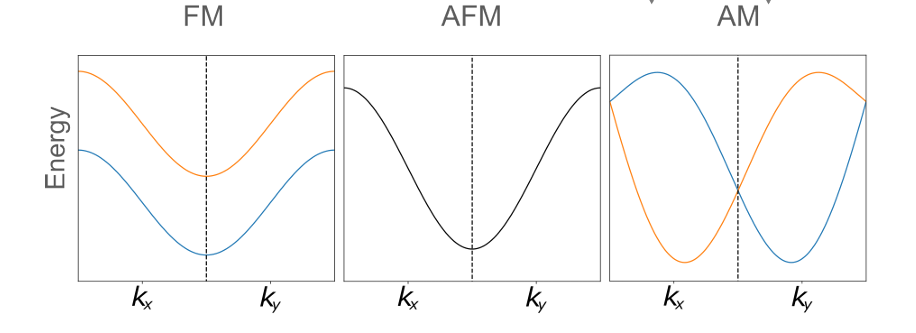
\includegraphics[width=\textwidth]{bands_altermagnet.png}
%         \caption{\footfullcite{visser2023}}
%     \end{figure}
% \end{frame}

% \begin{frame}{Theoretical approach}
%     \begin{enumerate}
%         \item Write classical equations of motion
%         \item Multiple scale expansion
%         \item Hamiltonian matrix for linear systems $\longrightarrow$ eigenmodes
%         \item Decouple motion in amplitude and phase $A=Re^{i\phi}$
%         \item ODEs for slow timescale 
%     \end{enumerate}
% \end{frame}

% \begin{frame}
%     \begin{tikzpicture}[>=Stealth, line width=1.2pt]

%     % --- Left Person (Passer) ---
%     \coordinate (L-head) at (0, 2.5);
%     \coordinate (L-pelvis) at (0, 1.2);
    
%     % Head & Torso
%     \draw[fill=white] (L-head) circle (0.25);
%     \draw (L-head) -- (L-pelvis);
%     % Legs
%     \draw (L-pelvis) -- (-0.4, 0);
%     \draw (L-pelvis) -- (0.2, 0);
%     % Arms (Extended forward releasing the ball)
%     \draw (0, 2.1) -- (0.5, 2.2) -- (0.8, 2.4);
%     \draw (0, 2.0) -- (0.5, 2.0) -- (0.9, 2.1);

%     % --- Right Person (Receiver) ---
%     \coordinate (R-head) at (5, 2.4);
%     \coordinate (R-pelvis) at (5, 1.2);
    
%     % Head & Torso
%     \draw[fill=white] (R-head) circle (0.25);
%     \draw (R-head) -- (R-pelvis);
%     % Legs (Slightly ready/bent stance)
%     \draw (R-pelvis) -- (4.6, 0);
%     \draw (R-pelvis) -- (5.3, 0);
%     % Arms (Reaching out to catch)
%     \draw (5, 2.0) -- (4.4, 2.1) -- (4.1, 2.3);
%     \draw (5, 1.9) -- (4.3, 1.9) -- (4.0, 2.1);

%     % --- The Basketball Trajectory & Motion Line ---
%     % Path coordinates for the arc
%     \coordinate (StartBall) at (0.9, 2.25);
%     \coordinate (MidBall) at (2.5, 3.4);
%     \coordinate (CurrentBall) at (3.5, 2.8);
    
%     % Motion/Wind Trail behind the ball
%     \draw[dashed, gray, line width=1pt] (StartBall) .. controls (1.5, 2.9) and (2.5, 3.4) .. (CurrentBall);
    
%     % Wind swoosh lines below the trajectory to emphasize speed/air flow
%     %\draw[thin, gray, ->] (1.2, 2.4) .. controls (1.8, 2.9) .. (2.4, 3.0);
%     %\draw[thin, gray, ->] (1.8, 2.8) .. controls (2.4, 3.2) .. (3.0, 3.1);

%     % --- The Basketball ---
%     % Base orange ball
%     \draw[fill=orange, draw=black] (CurrentBall) circle (0.22);
%     % Basketball Ribs/Lines
%     \draw[line width=0.6pt] (3.5, 3.02) -- (3.5, 2.58); % Vertical rib
%     \draw[line width=0.6pt] (3.28, 2.8) -- (3.72, 2.8); % Horizontal rib
%     \draw[line width=0.6pt] (3.35, 2.95) .. controls (3.5, 2.85) .. (3.65, 2.95); % Top curved rib
%     \draw[line width=0.6pt] (3.35, 2.65) .. controls (3.5, 2.75) .. (3.65, 2.65); % Bottom curved rib

%     % --- Ground Line ---
%     \draw[line width=0.8pt, gray!70] (-1, 0) -- (6.5, 0);

% \end{tikzpicture}
% \begin{tikzpicture}[>=Stealth, line width=1.2pt]

%     % --- Left Person (Now the Receiver) ---
%     \coordinate (L-head) at (0, 2.4);
%     \coordinate (L-pelvis) at (0, 1.2);
    
%     % Head & Torso
%     \draw[fill=white] (L-head) circle (0.25);
%     \draw (L-head) -- (L-pelvis);
%     % Legs (Ready stance)
%     \draw (L-pelvis) -- (-0.3, 0);
%     \draw (L-pelvis) -- (0.4, 0);
%     % Arms (Extended forward to receive)
%     \draw (0, 2.0) -- (0.6, 2.1) -- (0.9, 2.3);
%     \draw (0, 1.9) -- (0.7, 1.9) -- (1.0, 2.1);

%     % --- Right Person (Now the Passer) ---
%     \coordinate (R-head) at (5, 2.5);
%     \coordinate (R-pelvis) at (5, 1.2);
    
%     % Head & Torso
%     \draw[fill=white] (R-head) circle (0.25);
%     \draw (R-head) -- (R-pelvis);
%     % Legs
%     \draw (R-pelvis) -- (4.6, 0);
%     \draw (R-pelvis) -- (5.2, 0);
%     % Arms (Extended forward releasing the ball to the left)
%     \draw (5, 2.1) -- (4.5, 2.2) -- (4.2, 2.4);
%     \draw (5, 2.0) -- (4.5, 2.0) -- (4.1, 2.1);

%     % --- The Basketball Trajectory (Right to Left) ---
%     \coordinate (StartBall) at (4.1, 2.25);
%     \coordinate (MidBall) at (2.5, 3.4);
%     \coordinate (CurrentBall) at (1.5, 2.8);
    
%     % Motion/Wind Trail (Dashed gray, moving left)
%     \draw[dashed, gray, line width=1pt] (StartBall) .. controls (3.5, 2.9) and (2.5, 3.4) .. (CurrentBall);
    
%     % Wind swoosh lines below the trajectory showing leftward velocity
%     \draw[thin, gray, ->] (3.8, 2.4) .. controls (3.2, 2.9) .. (2.6, 3.0);
%     \draw[thin, gray, ->] (3.2, 2.8) .. controls (2.6, 3.2) .. (2.0, 3.1);

%     % --- The Basketball ---
%     \draw[fill=orange, draw=black] (CurrentBall) circle (0.22);
%     % Basketball Ribs/Lines
%     \draw[line width=0.6pt] (1.5, 3.02) -- (1.5, 2.58); 
%     \draw[line width=0.6pt] (1.28, 2.8) -- (1.72, 2.8); 
%     \draw[line width=0.6pt] (1.35, 2.95) .. controls (1.5, 2.85) .. (1.65, 2.95); 
%     \draw[line width=0.6pt] (1.35, 2.65) .. controls (1.5, 2.75) .. (1.65, 2.65); 

%     % --- Ground Line ---
%     \draw[line width=0.8pt, gray!70] (-1, 0) -- (6.5, 0);

%     % --- BIG RED BLOCKING CROSS (Signaling pass is not happening) ---
%     \coordinate (CrossCenter) at (2.5, 2.6);
%     \draw[line width=4pt, red, cap=round] ($(CrossCenter)+(-0.6,-0.6)$) -- ($(CrossCenter)+(0.6,0.6)$);
%     \draw[line width=4pt, red, cap=round] ($(CrossCenter)+(-0.6,0.6)$) -- ($(CrossCenter)+(0.6,-0.6)$);

% \end{tikzpicture}
% \end{frame}

% \begin{frame}[allowframebreaks]{Non-hermiticity}
%     \begin{itemize}
%         \item Motivation: gain/loss for pendula chirality, non-reciprocal hopping 
%         \item In hermitian systems: PBC bulk $\longrightarrow$ OBC edge states
%         \item In non-hermitian systems: extreme sensitivity to boundaries 
%         \item Spectrum becomes complex
%          \begin{figure}
%             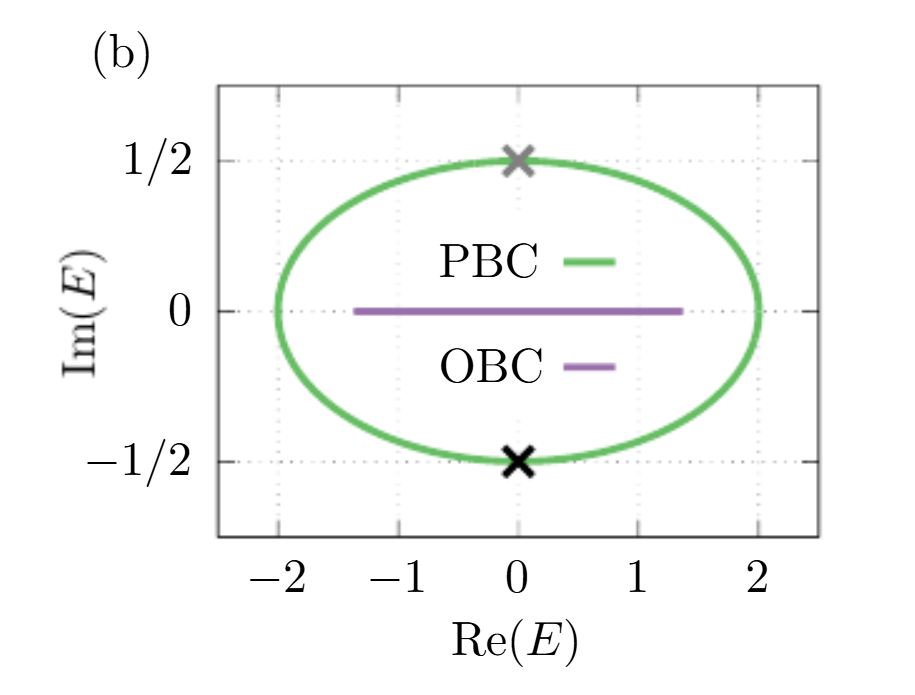
\includegraphics[width = 0.4\textwidth]{hatano-nelson_spectrum.png}
%             \caption{\footfullcite{Gohsrich_2025}}
%         \end{figure}
%         \item \textbf{New} non-hermitian skin effect: eigenstates localize at boundary 
%         \item Example: Hatano-Nelson model  
%         \begin{align*}
% \hat{H}_{\rm HN} = \sum_j \left[ t_Rc_{j+1}^{\dagger} c_j + t_Lc_j^{\dagger} c_{j+1} \right]
% \end{align*}
%     \end{itemize}
% \end{frame}

% \begin{frame}{Non-reciprocity}
%         \begin{minipage}[t]{0.65\textwidth}
%         \begin{itemize}
%             \item Meaning: asymmetric interaction 
%             \item Example: diode
%             \item Motivation: breaks inversion symmetry $\longrightarrow$ directional waves  
%             %\item Response differs when transmitter/receiver swapped \pause
%             %\item Breaks Newton's third law (classical level) \pause
%             \item $\begin{pmatrix}
%             F_1 \\ 
%             F_2
%             \end{pmatrix}
%             =
%             \begin{pmatrix}
%             k & -k^o \\ 
%             +k^o & k
%             \end{pmatrix}
%             \begin{pmatrix}
%             \Delta_1 \\ 
%             \Delta_2
%             \end{pmatrix}$ \pause 
%             \item Non-reciprocal units 
%             %\item Leads to pendula chirality
%         \end{itemize}
%     \end{minipage}%
%     \hfill
%     \begin{minipage}[t]{0.3\textwidth}
%         \vspace{0.5cm}
%         \raggedleft
%         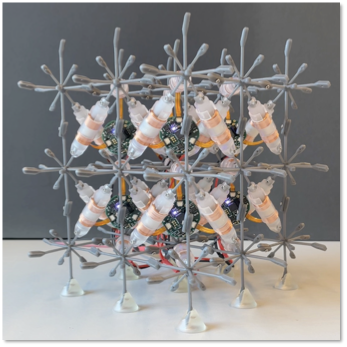
\includegraphics[width=\linewidth]{Yuan_cube_clear.png}
%         %\caption{}
%     \end{minipage}
% \end{frame}

% \begin{frame}[allowframebreaks]{Non-reciprocity}
%         \begin{itemize}
%             \item Meaning: asymmetric interaction 
%             \item Example: diode
%             \item Motivation: breaks inversion symmetry $\longrightarrow$ directional waves  
%             %\item Response differs when transmitter/receiver swapped \pause
%             %\item Breaks Newton's third law (classical level) \pause
%             \item $\begin{pmatrix}
%             F_1 \\ 
%             F_2
%             \end{pmatrix}
%             =
%             \begin{pmatrix}
%             k & -k^o \\ 
%             +k^o & k
%             \end{pmatrix}
%             \begin{pmatrix}
%             \Delta_1 \\ 
%             \Delta_2
%             \end{pmatrix}$ \pause 
%         \begin{figure}
%             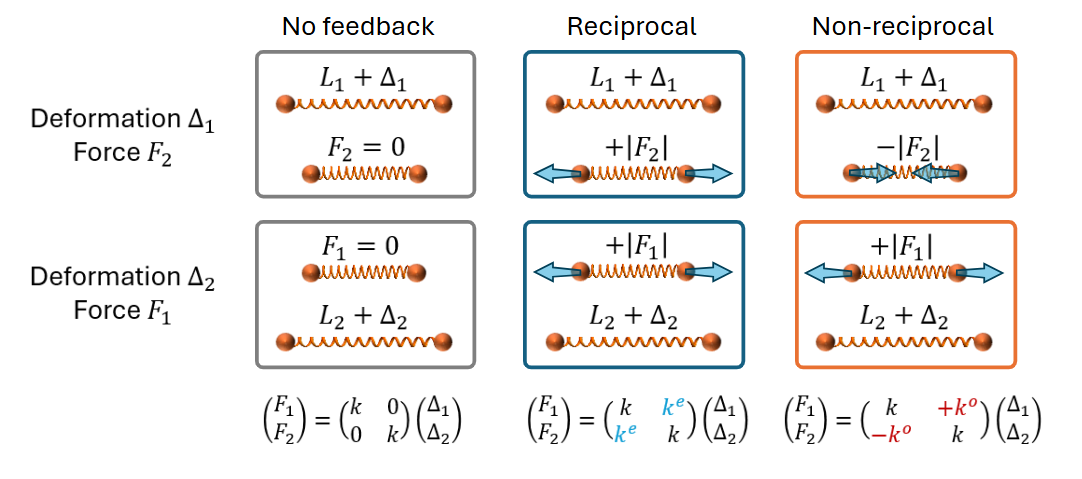
\includegraphics[width=0.8\textwidth]{non_reciprocal_spring_actuators.png}
%             \caption{Non-reciprocal actuators}
%         \end{figure}
%         \framebreak 
%         \item Non-reciprocal units 
%             %\item Leads to pendula chirality
%         \end{itemize}
%         \begin{figure}
%             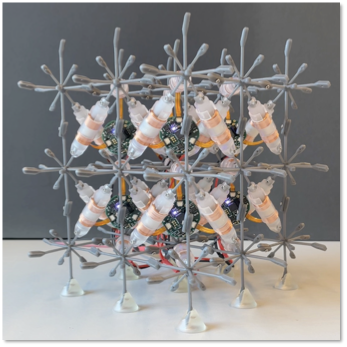
\includegraphics[width=0.5\linewidth]{Yuan_cube_clear.png}
%             \caption{3d cube}
%         \end{figure}
        
% \end{frame}


% \begin{frame}{Non-reciprocity leads to limit cycles}
%      EOM of two non-reciprocally coupled actuators:
%     \begin{align}
%         \xdd_1 +k_0x_1 +  \gamma \xd_1 + k_cx_1^3 + k_ax_2 = 0 \\ 
%         \xdd_2 +k_0x_2 +  \gamma \xd_2 + k_cx_1^3 - k_ax_1 = 0 
%     \end{align}
%     \begin{columns}[t]
%         \begin{column}{0.6\textwidth}
%     \begin{alertblock}{Control parameter}
%         Activity/gain $k_a$
%     \end{alertblock}
%     \begin{itemize}
%     \item If $|k_a|<\gamma \sqrt{k_0}$, oscillations die
%     \item If $|k_a|>\gamma \sqrt{k_0}$, stable limit cycles, with chirality \begin{enumerate}
%         \item[a] $k_a>0$ counterclockwise 
%         \item[b] $k_a<0$ clockwise 
%     \end{enumerate}
%     \end{itemize}
%         \end{column}
%     \begin{column}{0.35\textwidth}
%         \begin{figure}
%         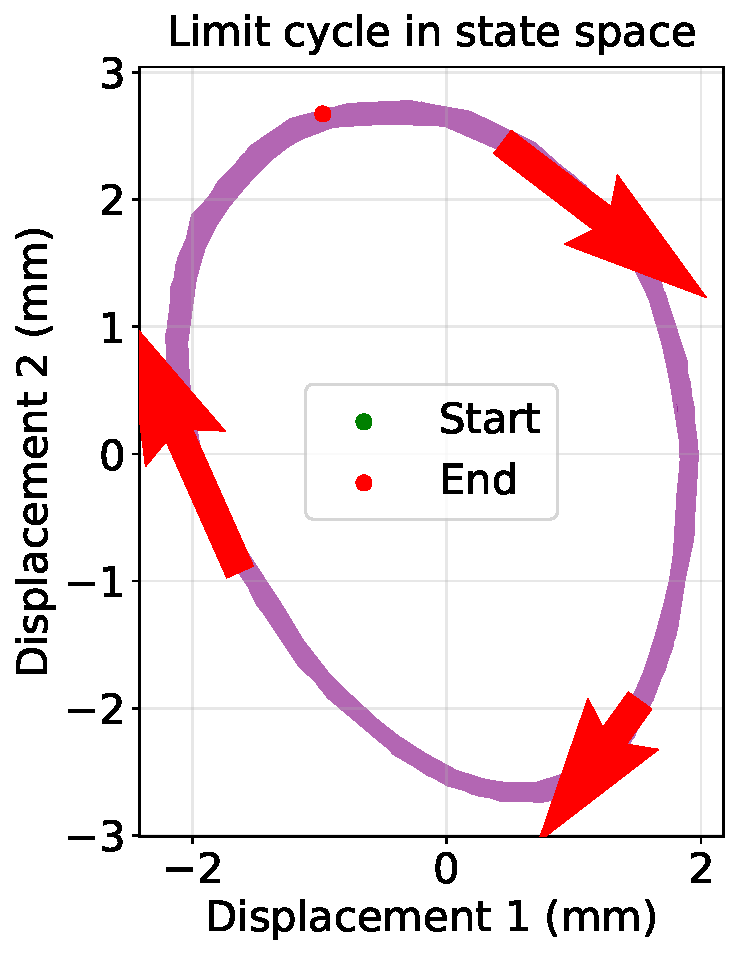
\includegraphics[width=\textwidth]{limit_cycle_example.pdf}
%     \end{figure}
%     \end{column}
%     \end{columns}
% \end{frame}

% \begin{frame}{Supercritical Hopf bifurcation}
%     \begin{figure}
%     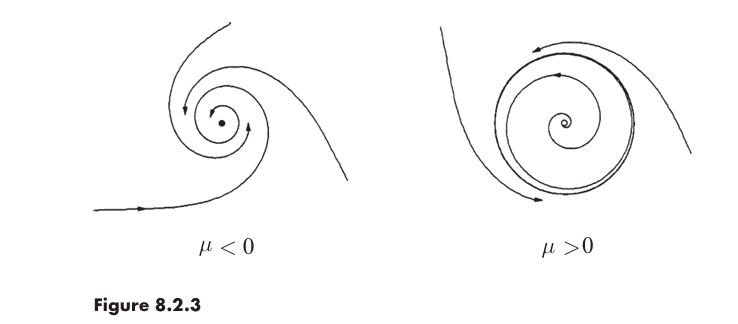
\includegraphics[width=0.7\textwidth]{supercritical_Hopf_bifurcation_diagram.PNG}
% \end{figure}
% Theoretical predictions: 
% \begin{itemize}
%     \item Exceptional point $k_a^c = \gamma \sqrt{k_0}$
%     \item Frequency $\omega = \frac{k_a}{\gamma}$
%     \item Amplitude $R \sim \sqrt{\frac{2k_a^c}{k_c\gamma^2}(k_a-k_a^c)}$
% \end{itemize}
% \end{frame}

% \begin{frame}[noframenumbering]{Activity}
%     The classical analogue of non-hermiticity of Hatano-Nelson is non-reciprocity. \pause
%     \vfill
%     Activity: internal energy source. \pause 
%     \vfill
%     There are different ways to achieve activity:  \pause
%     \begin{itemize}
%         \item Negative damping \pause
%         \item Time delay \pause 
%         \item \textbf{Non-reciprocity}
%     \end{itemize}
% \end{frame}

% \begin{frame}[noframenumbering]{2 interacting non-reciprocal pendula}
%     \begin{figure}
%         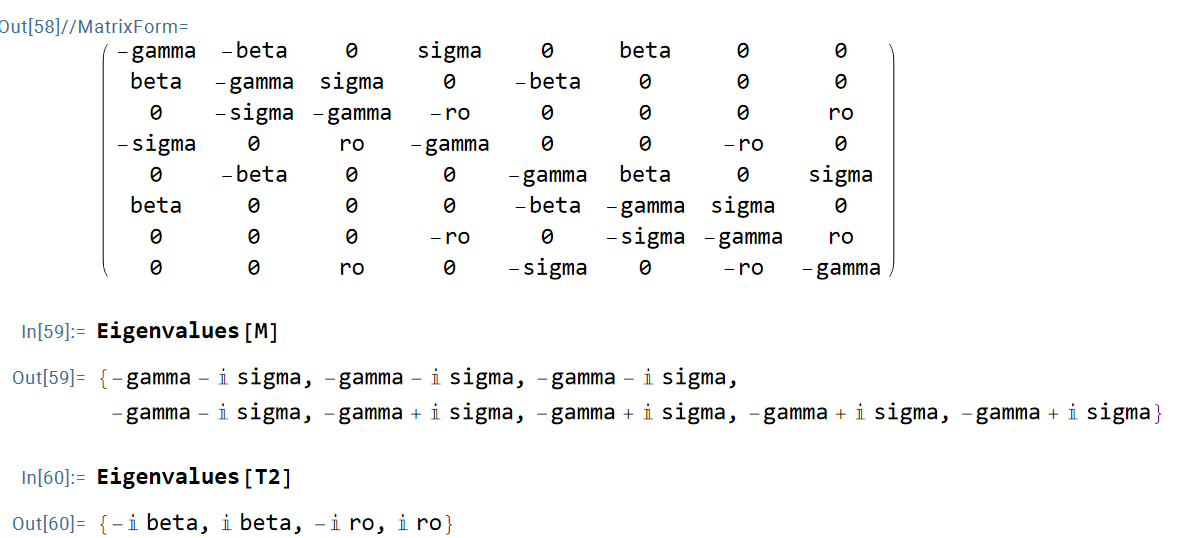
\includegraphics[width = \textwidth]{2NRpendula.png}
%     \end{figure}
% \end{frame}

% \begin{frame}[noframenumbering]{Mechanical altermagnet}
%     \begin{itemize}
%         \item Focus on anisotropic wave propagation feature of altermagnets
%         \item Exp: build on Amber's work: stack 2 toy layers
%         \item Th: construct model and explain observations
%         \item Study propagation of waves
%         \item Main source: Amber's thesis
%         %\item Best case scenario: 
%         %\item PROS: 
%         %\item CONS: 
%     \end{itemize}
%     \begin{figure}
%         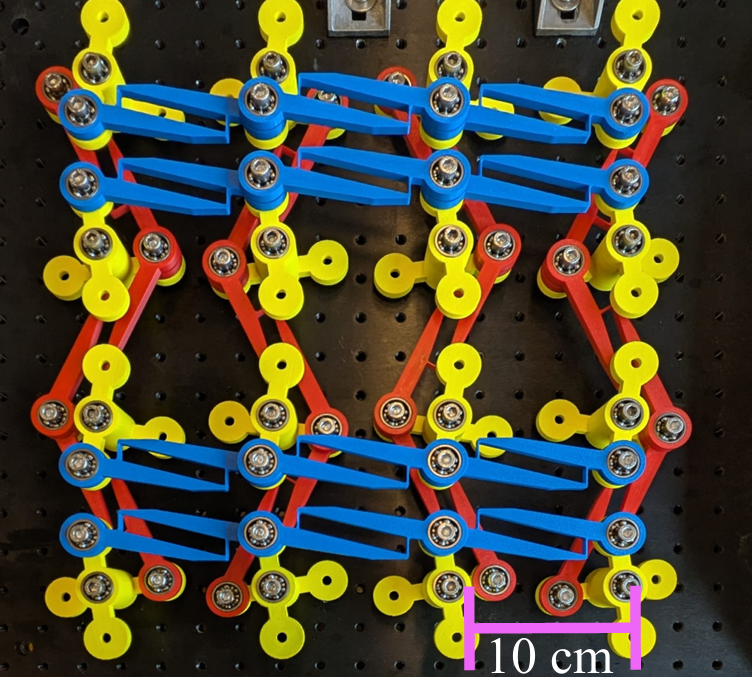
\includegraphics[width=0.5\textwidth]{mechanical_AM_Amber_toy.png}
%     \end{figure}
% \end{frame}

% \begin{frame}[noframenumbering]{Piezoelectric}
%     \begin{itemize}
%         \item Exp: build altermaterial using capacitors with piezoelectric response
%         \item Th: construct microscopic quantum model and compare
%         \item Auxetic piezo
%         \item Best case scenario: show piezoelectric properties of alterelectrics
%         \item Review by Gao, Sharma
%     \end{itemize}
%     \begin{figure}
%         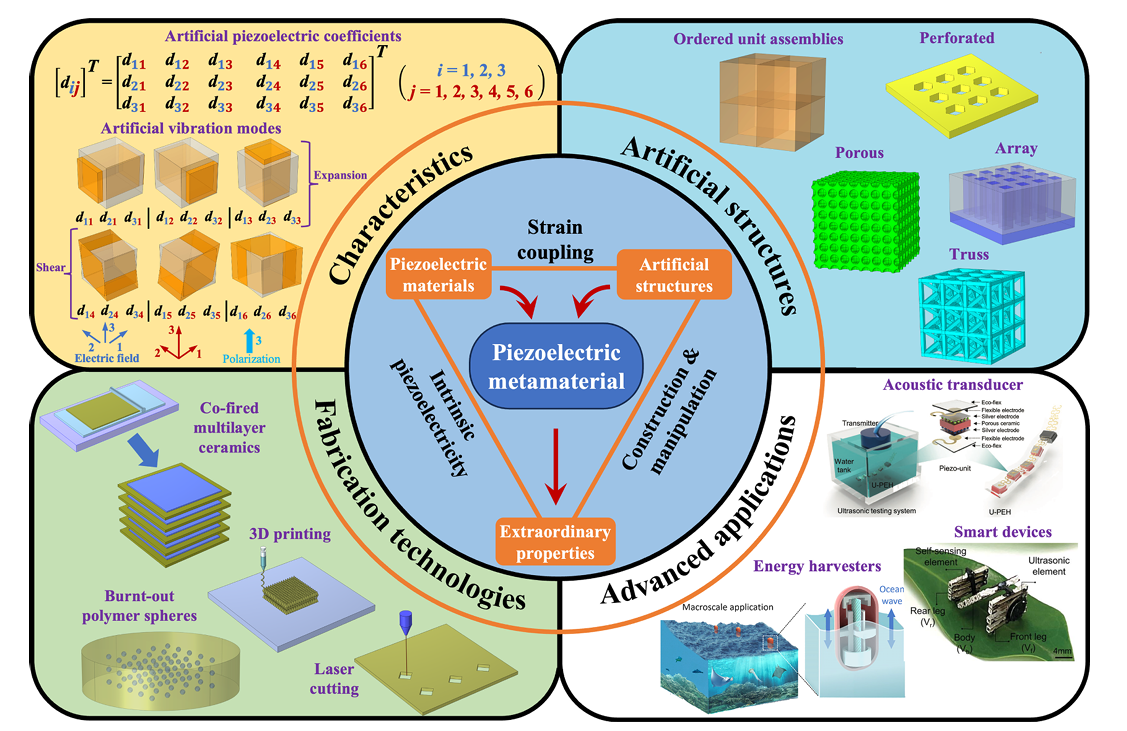
\includegraphics[width=0.5\textwidth]{piezoelectric_metamaterials.png}
%     \end{figure}
% \end{frame}

% \begin{frame}[noframenumbering]{Non-hermiticity}
%     \begin{itemize}
%         \item Combine altermagnetic symmetry with non-hermiticity
%         \item Exp: stack Yuan's cubes with odd elasticity
%         \item Study waves propagating
%         \item Gain-momentum locking
%         \item Th: write analogous quantum hamiltonian and analyse it
%     \end{itemize}
%      \begin{figure}
%         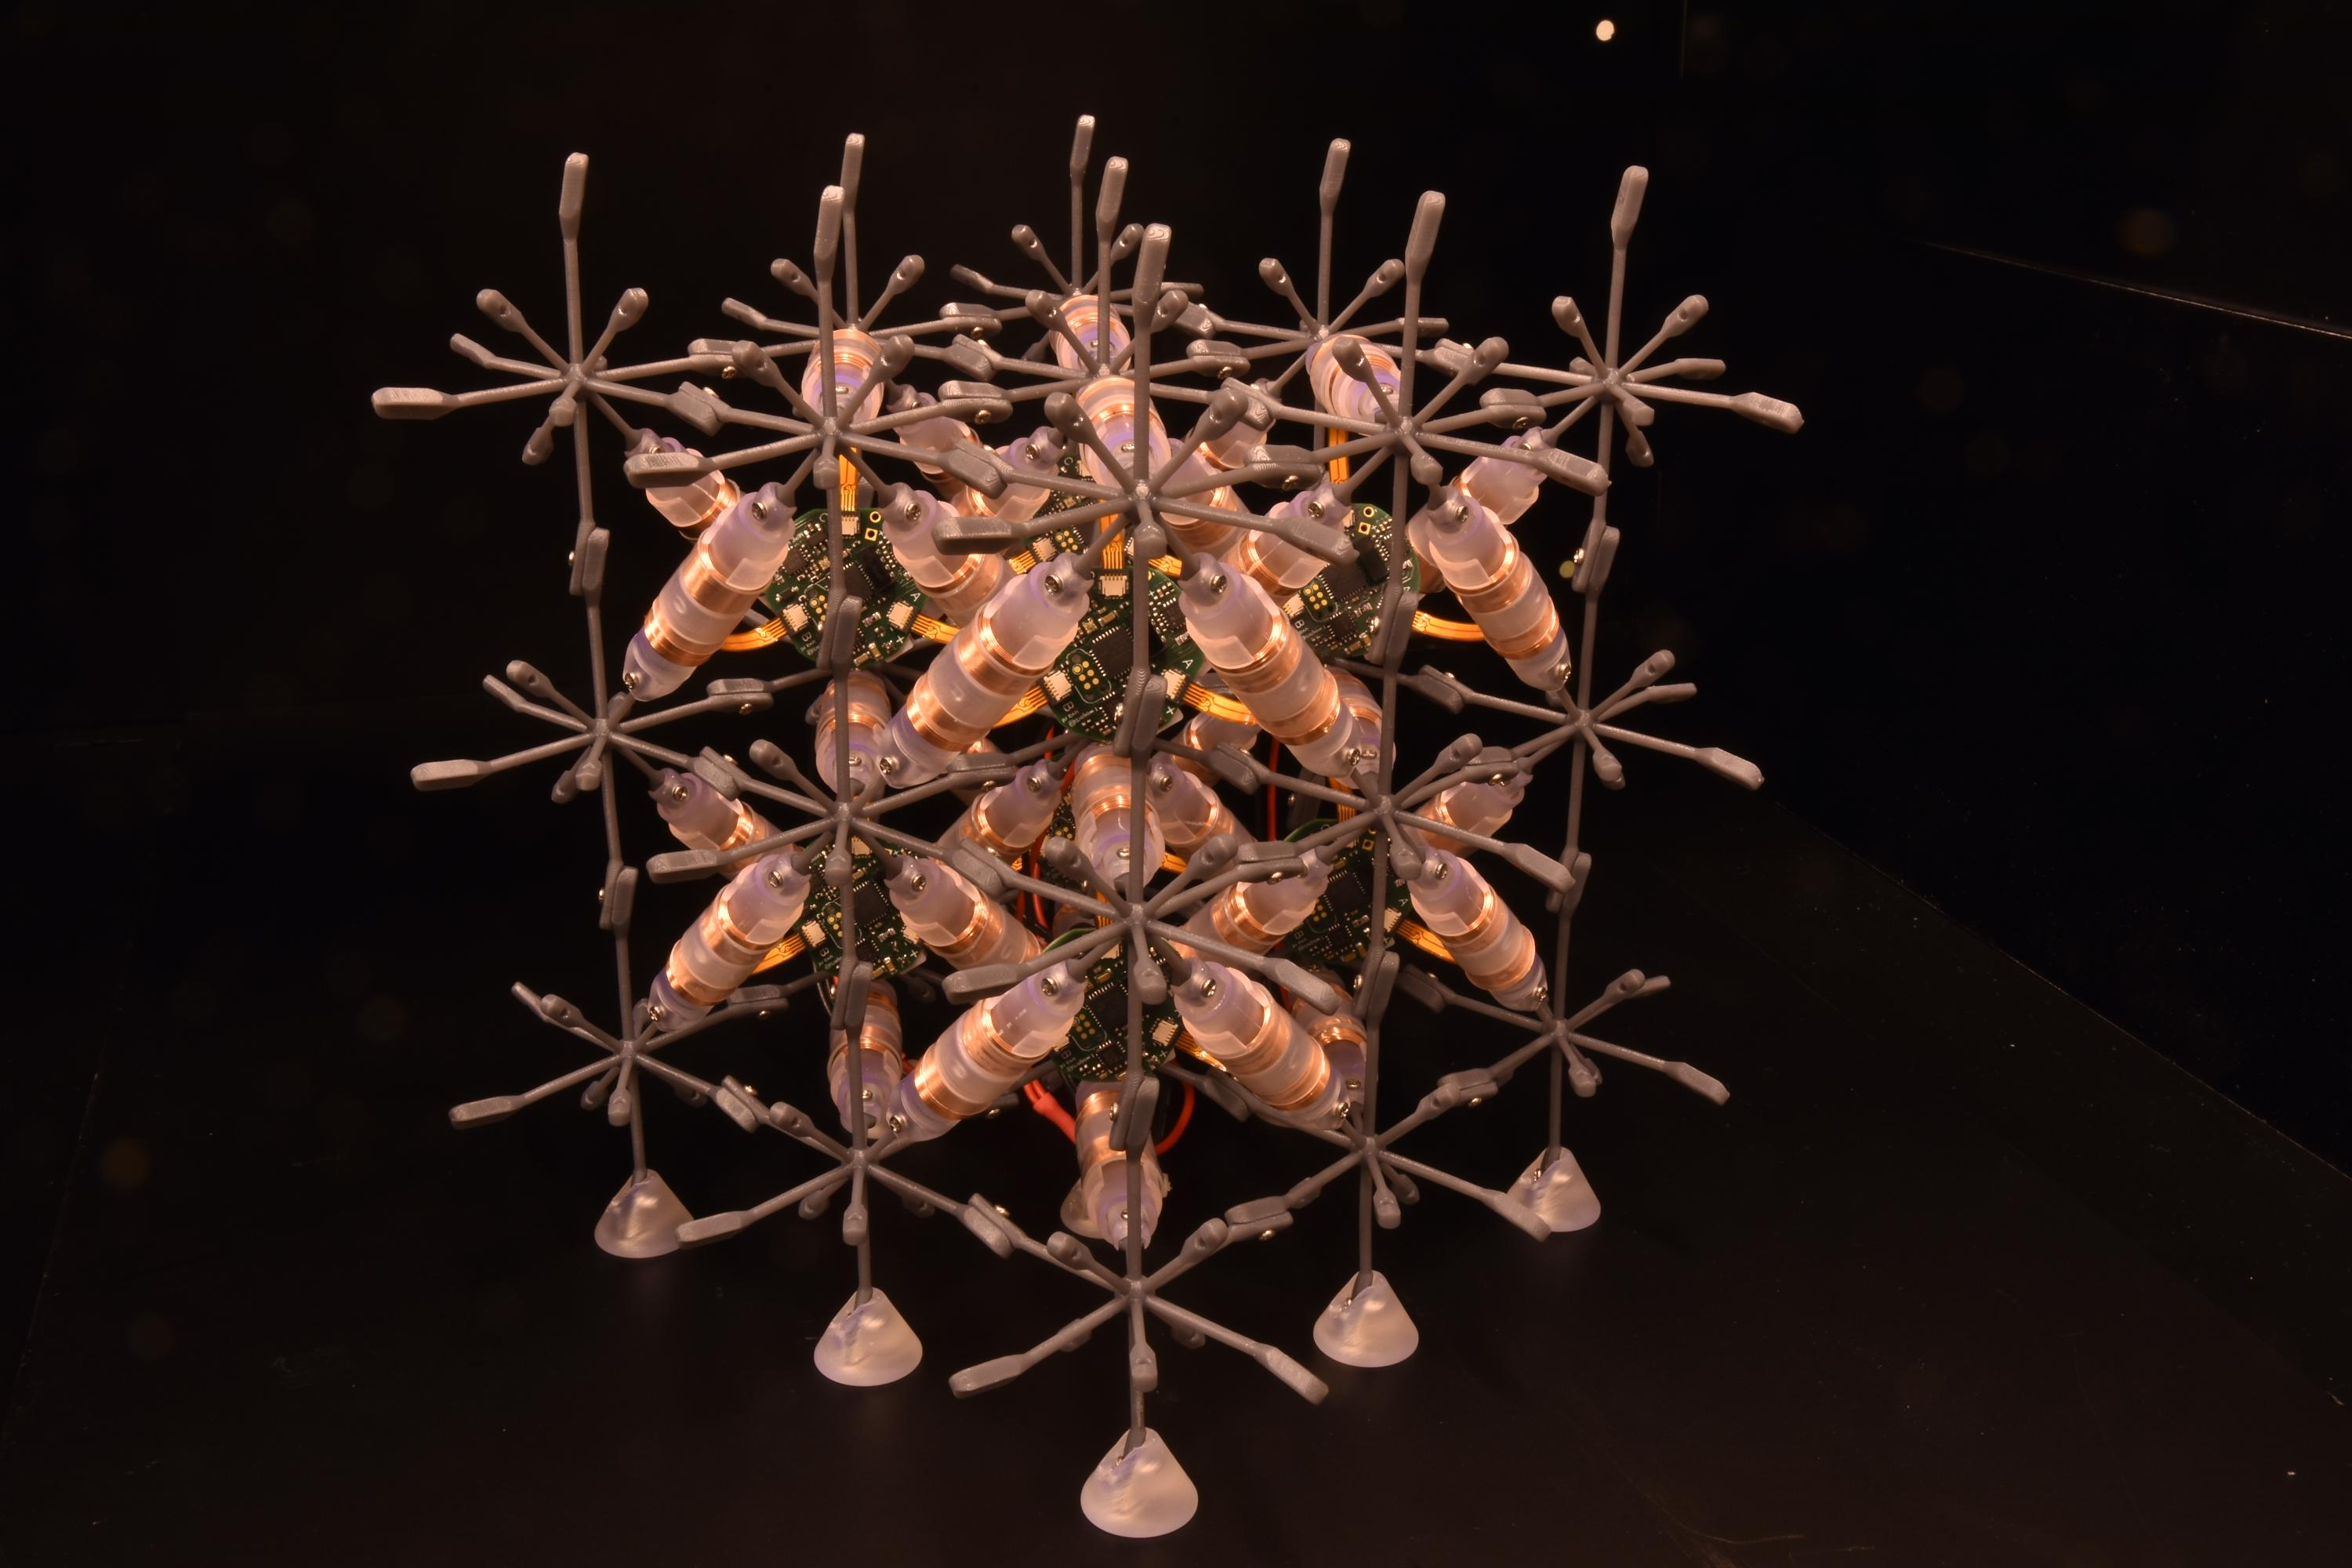
\includegraphics[width=0.5\textwidth]{Yuan_robot.jpeg}
%     \end{figure}
% \end{frame}

% \begin{frame}[noframenumbering]{Other}
%     \begin{itemize}
%         \item Metamaterials with higher order altermagnet symmetries
%         \item Consider other rotations besides 90º
%         \item For theory in general: band structure, ground state, excitations, topological properties, defects
%     \end{itemize}
% \end{frame}

% \begin{frame}[noframenumbering]{Research plan}
%     \begin{itemize}
%         \item Calculate band structure of mechanical Lieb lattice
%         \item Simulate Lieb lattice of non-reciprocal units
%         \item Build Lieb lattice of non-reciprocal units
%     \end{itemize}
%     Possible questions
%     \begin{itemize}
%         \item Are there skin effects?
%     \end{itemize}
% \end{frame}

% \begin{frame}[noframenumbering]{Do altermagnets always have hyperbolic dispersion?}
%     \pause
%     \begin{enumerate}
%         \item Break TRS \pause
%         \item C4T symmetry \pause
%         \item Inversion symmetry \pause
%         \item Zero magnetisation
%     \end{enumerate}
% \end{frame}

% \begin{frame}[noframenumbering]{Hatano-Nelson ladder}
%     Parameters: U = 1, r = 2, t = 1, a = 1
%     \begin{figure}
%         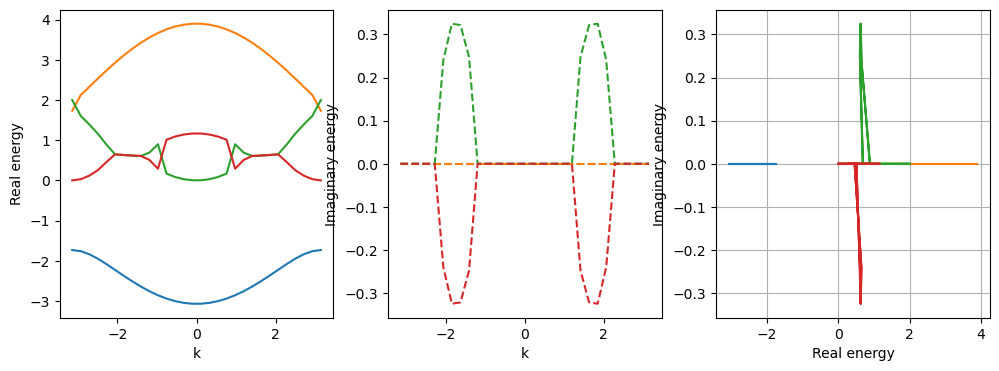
\includegraphics[width=\textwidth]{hatano_ladder_spectrum.png}
%     \end{figure}
%     \begin{figure}
%         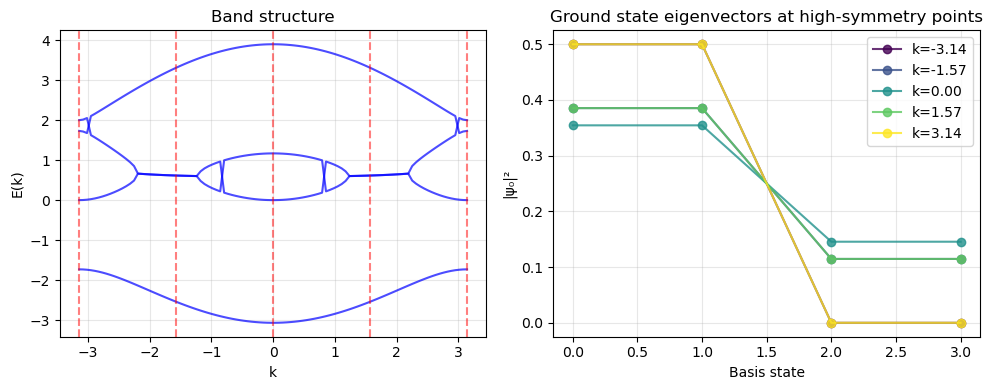
\includegraphics[width=0.5\textwidth]{hatano_ladder_eigenstates.png}
%     \end{figure}
% \end{frame}

% \begin{frame}[noframenumbering]
% \begin{figure}
%     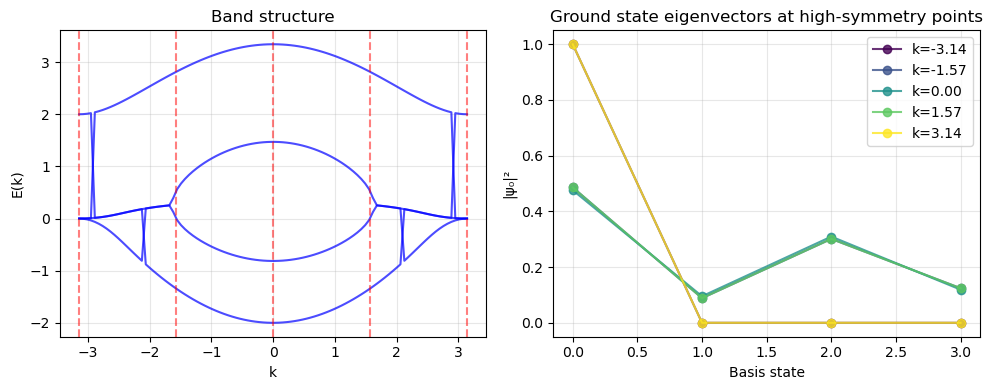
\includegraphics[width=\textwidth]{hatano_ladder_asymmetric.png}
% \end{figure}
% \end{frame}

% \begin{frame}{In practice}
%     \begin{alertblock}{What is the project about?}
%         Altermagnetic symmetry/Lieb lattice + non-hermiticity/non-reciprocity, in classical analogues
%     \end{alertblock} \pause 
%     The procedure has been:  
%     \begin{enumerate}
%         \item Choose a classical model   
%         \item Write equations of motion   
%         \item Map to quantum system (using mulitple scale expansion) 
%         \item Analyze spectrum and eigenstates \pause 
%     \end{enumerate}
%     \vfill
%     The idea is to apply them to increasingly more complex models.
%     \vfill
%     \begin{block}{Experimentally}
%         Build a Lieb lattice of non-reciprocal pendula and compare with theoretical predictions
%     \end{block}
% \end{frame}

% \begin{frame}[noframenumbering, allowframebreaks]{Multiple scale expansion: the map to quantum system}
%     Technique useful for solving nonlinear ODEs with different timescales \\
%     \vspace{0.5cm}
%     Simple example: weakly damped harmonic oscillator \\ $\xdd + x +2\varepsilon\xd =0$ \\
%     \vspace{0.5cm}
%     How do we approximate solution? With a power series in $\varepsilon$: \\ 
%     $x = x_0(t) + \varepsilon x_1(t) + \bigO(\varepsilon^2)$ \\
%     \vspace{0.5cm}
%     Substituting $[\xdd_0+x_0]+\varepsilon[\xdd_1+x_1+2x_0]+\bigO(\varepsilon^2)=0$ \\
%     \vspace{0.2cm}
%     Solution: $x(t,\varepsilon) = \sin{t} -\varepsilon t\sin{t}+\bigO(\varepsilon^2)$ \\
%     \framebreak
%     Can we find an approximate solution valid for $t>\bigO(1/\varepsilon)$? \\
%     \vspace{0.2cm}
%     Define 2 timescales: $\tau=t$ and $t=\frac{T}{\varepsilon}$ \\
%     \vspace{0.2cm}
%     Rewrite solution: $x(t,\varepsilon)=x_0(\tau,T)+\varepsilon x_1(\tau,T)+\bigO(\varepsilon^2)$ \\
%     \vspace{0.2cm}
%     Time derivative: $\xd = \partial_\tau x_0+\varepsilon(\partial_T x_0+\partial_\tau x_1)+\bigO(\varepsilon^2)$ \\
%     \vspace{0.2cm}
%     $\bigO(\varepsilon^0)$: $\partial_{\tau\tau}x_0+x_0=0\longrightarrow x_0=A(T)\sin{\tau}+B(T)\cos{\tau}$ \\
%     \vspace{0.1cm}
%     $\bigO(\varepsilon)$: $\partial_{\tau\tau}x_1+x_1=-2(\partial_{T\tau}x_0+\partial_\tau x_0)$ \\
%     \vspace{0.2cm}
%     We require no secular terms $\longrightarrow A'+A=0\; B'+B =0$ \\
%     \vspace{0.3cm}
%     Approximate solution: $x = e^{-\varepsilon t}\sin{t} +\bigO()$ \\
%     \vspace{0.3cm}
%     Note: this technique is much more general.
% \end{frame}


% \begin{frame}{Classical to quantum}
%     Assumption: treat non-harmonic terms weakly $\longrightarrow \varepsilon$ \\
%     \vspace{0.3cm}
%     Oscillating solutions with (slow) time-dependent coefficients \\
%     \vspace{0.3cm}
%     The coefficients evolve as $\vec{A}' = M\vec{A}$ \\
%     \vspace{0.3cm}
%     Map to a Schrödinger equation with Hamiltonian $H=iM$ \\
%     \vspace{0.3cm}
%     Use CMT knowledge to analyse system: spectrum and eigenstates
% \end{frame}

% \begin{frame}{Non-reciprocal pendulum}
%     \begin{align}
%         \xdd +kx + \epsilon \gamma \xd +\epsilon k^ay = 0 \\
%         \ydd +ky + \epsilon \gamma \yd -\epsilon k^ax = 0 
%     \end{align}
%     The energies are 
%     \begin{align}
%         \text{clockwise - decay} \; E_1 = -\frac{i}{2}\left(\gamma + \frac{k^a}{\sqrt{k}}\right) \\
%         \text{anticlockwise - grow} \; E_2 = \frac{i}{2}\left(-\gamma + \frac{k^a}{\sqrt{k}}\right)
%     \end{align}
%     $E_1$ has 2 eigenvectors rotating clockwise with different initial phase- these modes decay.
%     $E_2$ has 2 eigenvectos that rotate anticlockwise with different initial phase- these modes grow.
% \end{frame}

% \begin{frame}{2 coupled non-reciprocal pendula}
%     \begin{figure}
%         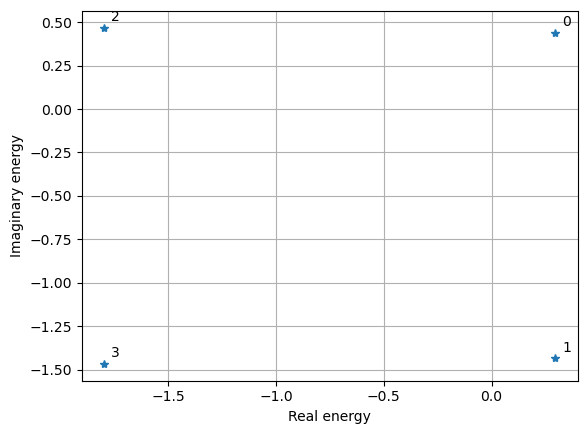
\includegraphics[height=3cm, width=0.5\textwidth]{2NR_coupled_pendula_spectrum.png}
%     \end{figure}
%     \begin{figure}
%         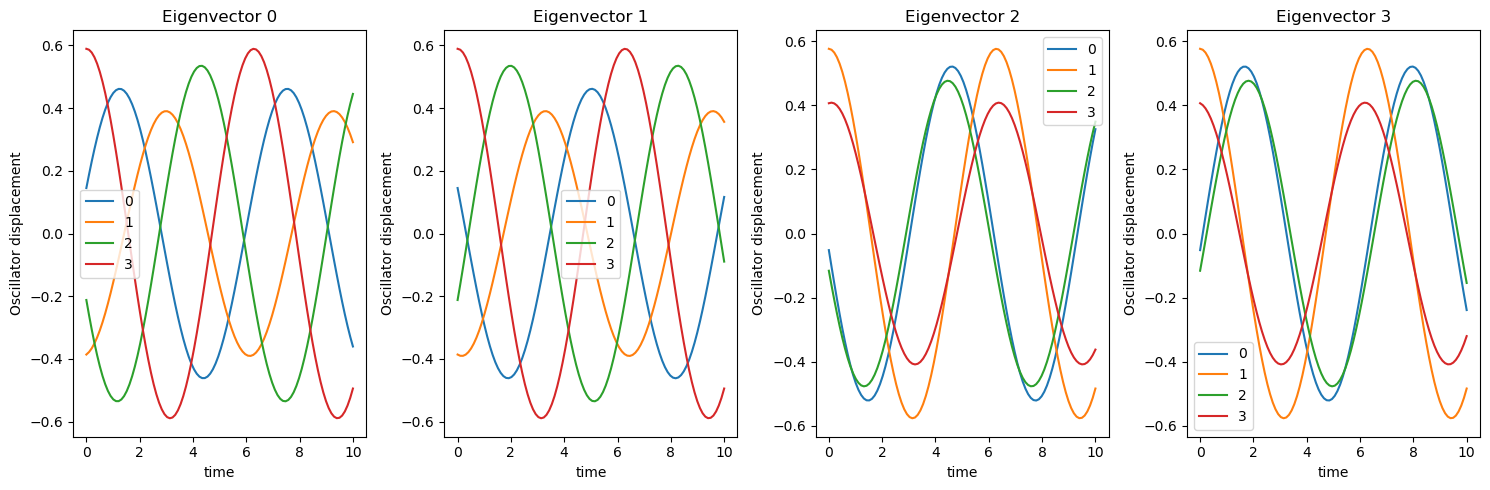
\includegraphics[height=3cm, width=\textwidth]{2NR_coupled_pendula_eigenvectors.png}
%     \end{figure}
% \end{frame}

% \begin{frame}[allowframebreaks]{Lieb lattice of non-reciprocal pendula}
%     % We consider a Lieb lattice of non-reciprocal pendula. 
%     % \begin{figure}
%     %     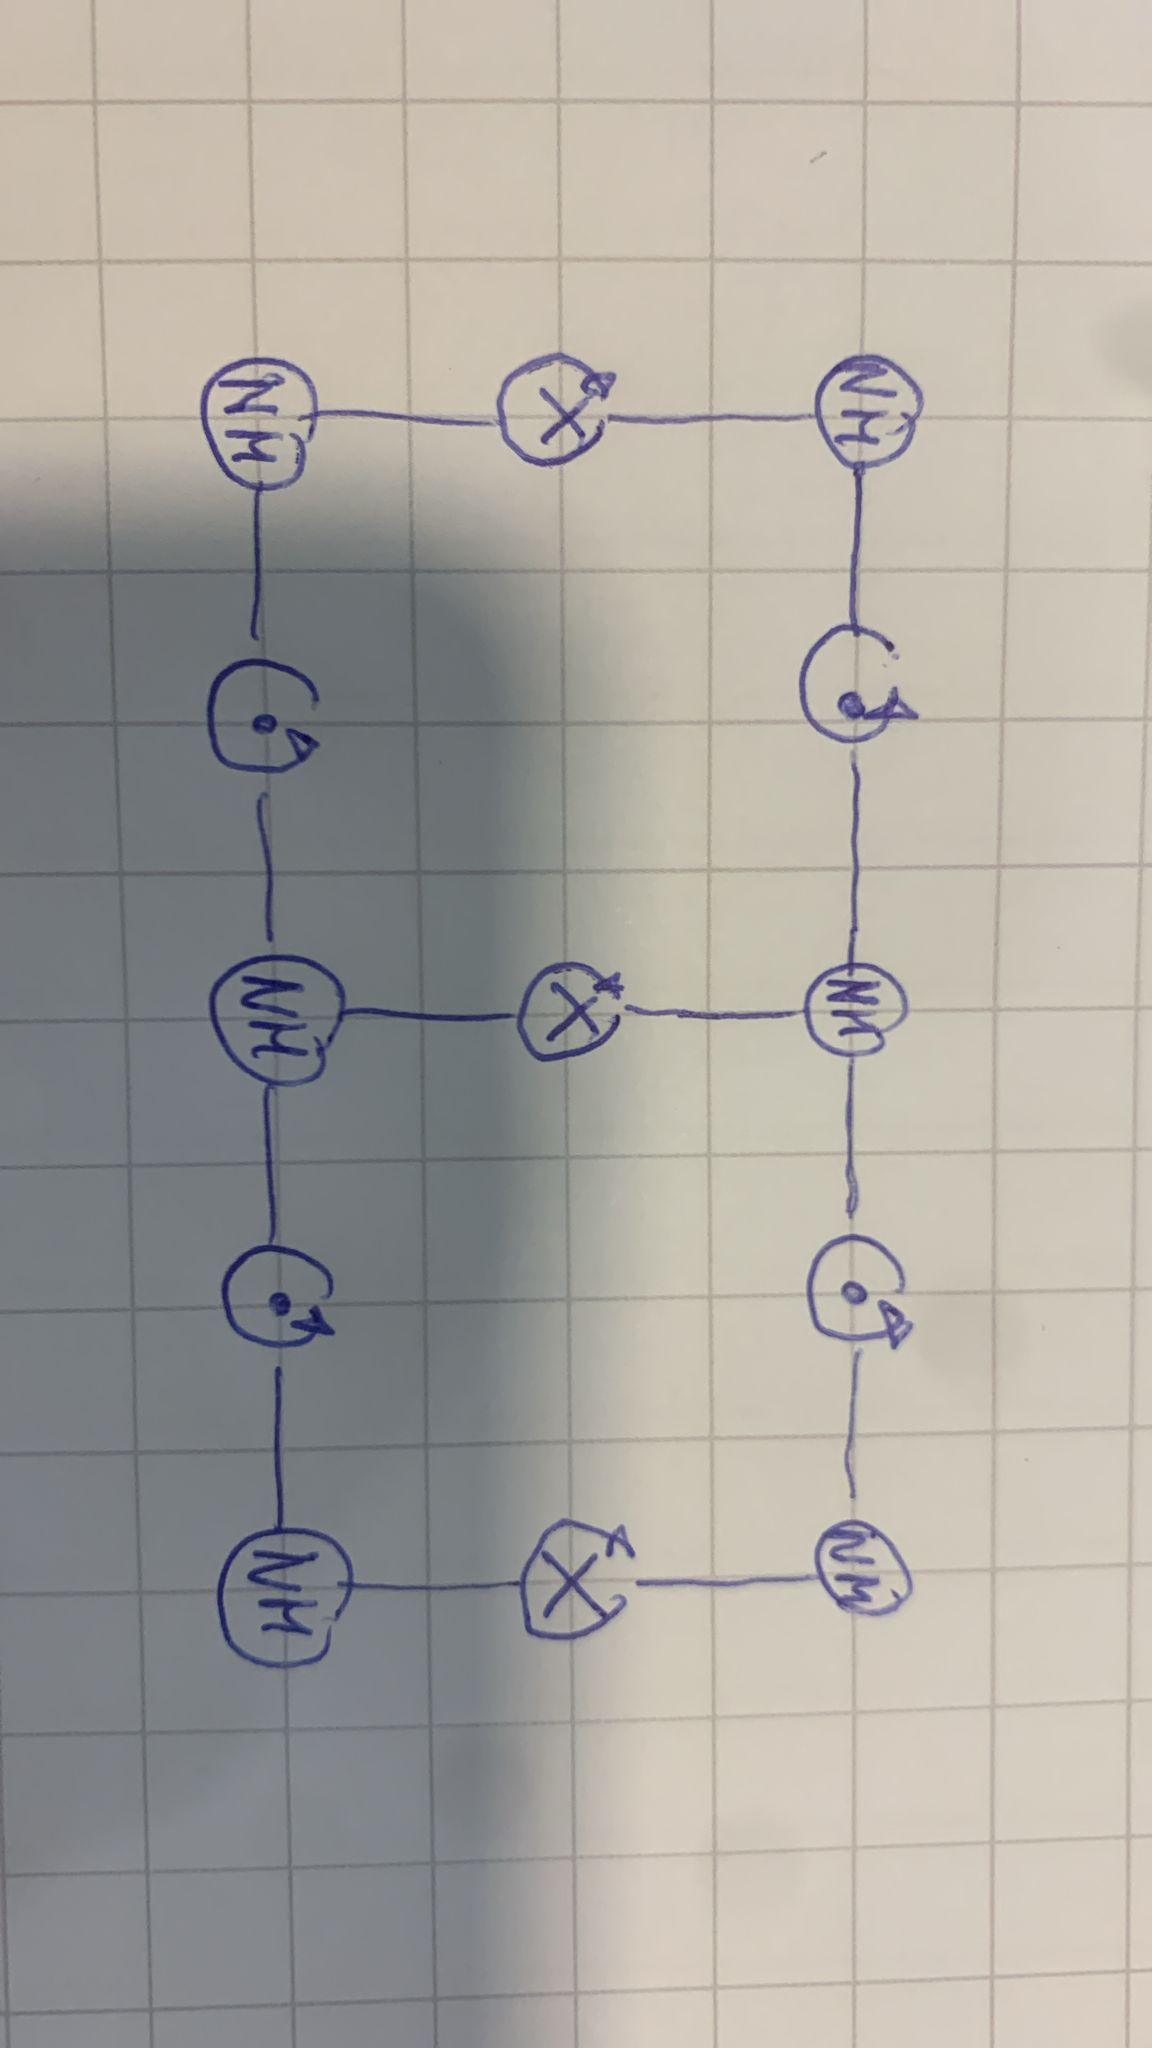
\includegraphics[rotate=90, width = 0.5\textwidth]{WhatsApp Image 2025-10-10 at 12.15.01.jpeg}
%     % \end{figure}
%     % \framebreak 
%     It seems like there are modes with zero energy in certain directions %- the band is flat; but not at E=0, 
%     % I guess you can tune that with chemical potential \\
%     % Other bands look more nomral with somewhat well shape \\
%     Real spectrum:
%     \begin{figure}
%         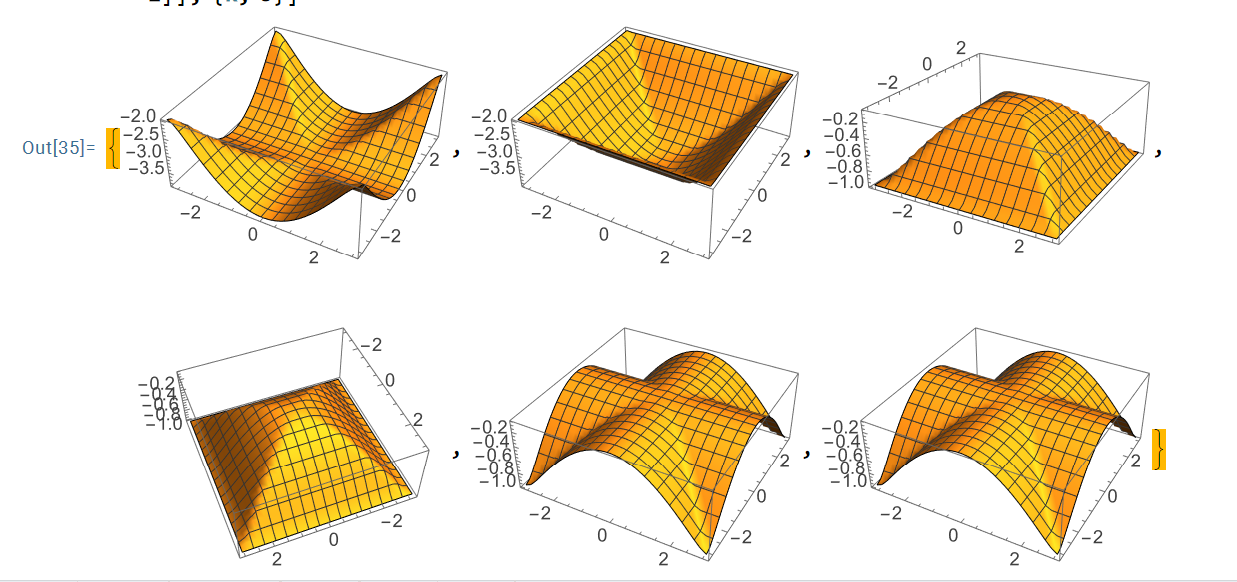
\includegraphics[width = 0.5\textwidth]{non_reciprocal_Lieb_real_energies.png}
%     \end{figure}
%     %\framebreak 
%     Imaginary spectrum:
%     \begin{figure}
%         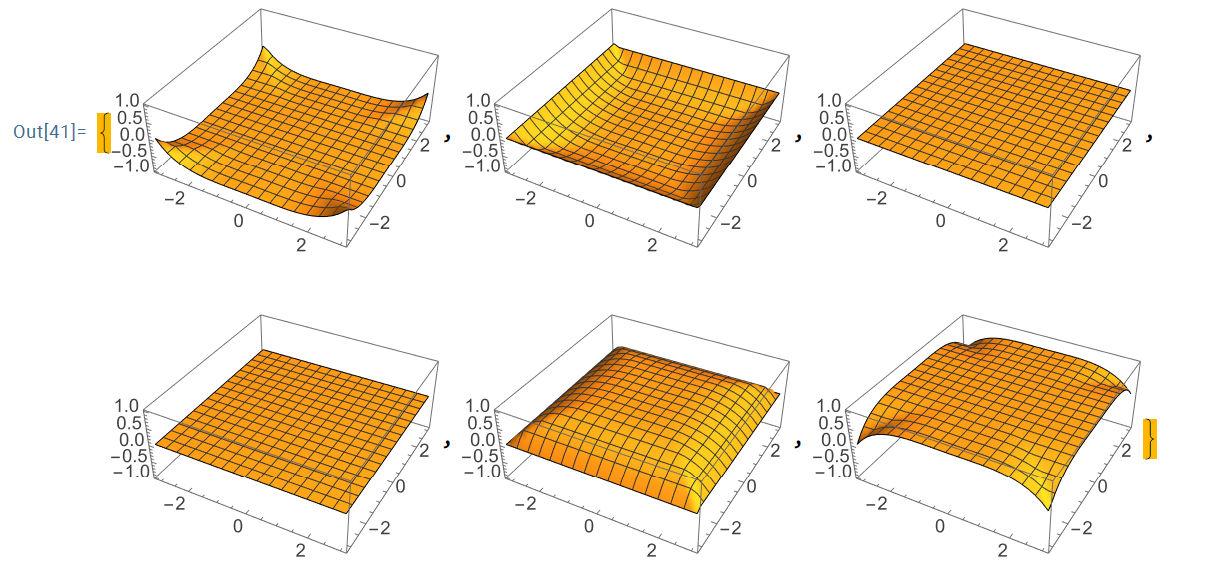
\includegraphics[width = 0.5\textwidth]{non_reciprocal_Lieb_imag_energies.png}
%     \end{figure}
% \end{frame}

% \begin{frame}{Hatano-Nelson ladder PBC}
%     \begin{figure}
%         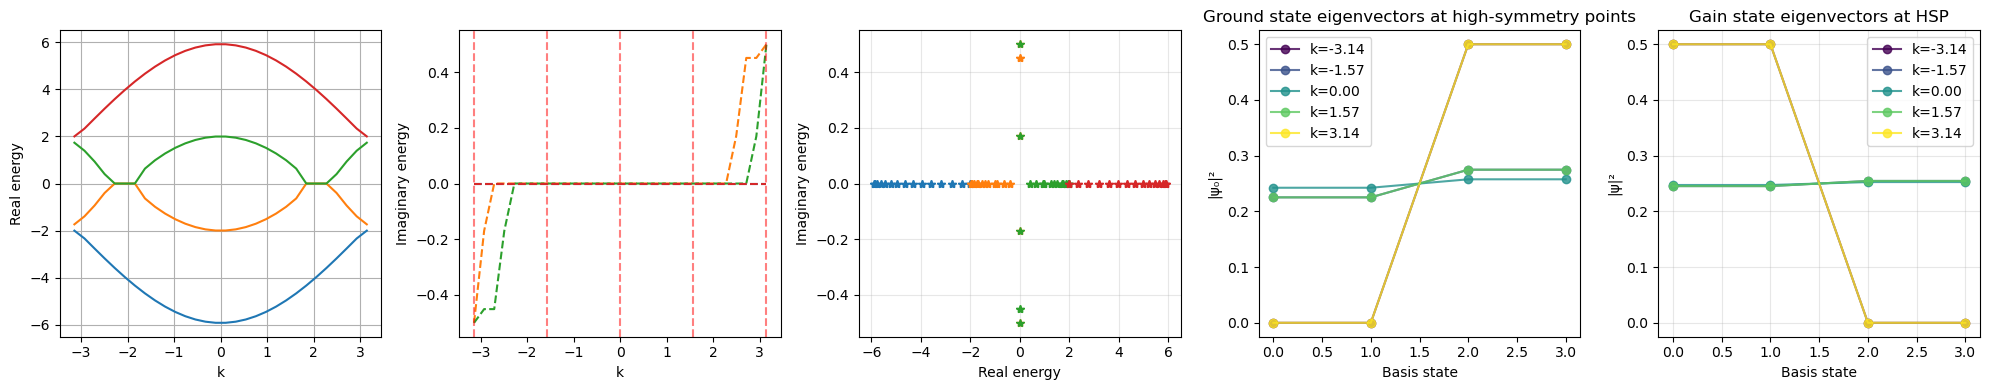
\includegraphics[width=\textwidth]{H-N_ladder_PBC_imaginarypotential.png}
%         \caption{Hatano-Nelson ladder PBC with imaginary onsite potential.}
%     \end{figure}
%     \begin{figure}
%         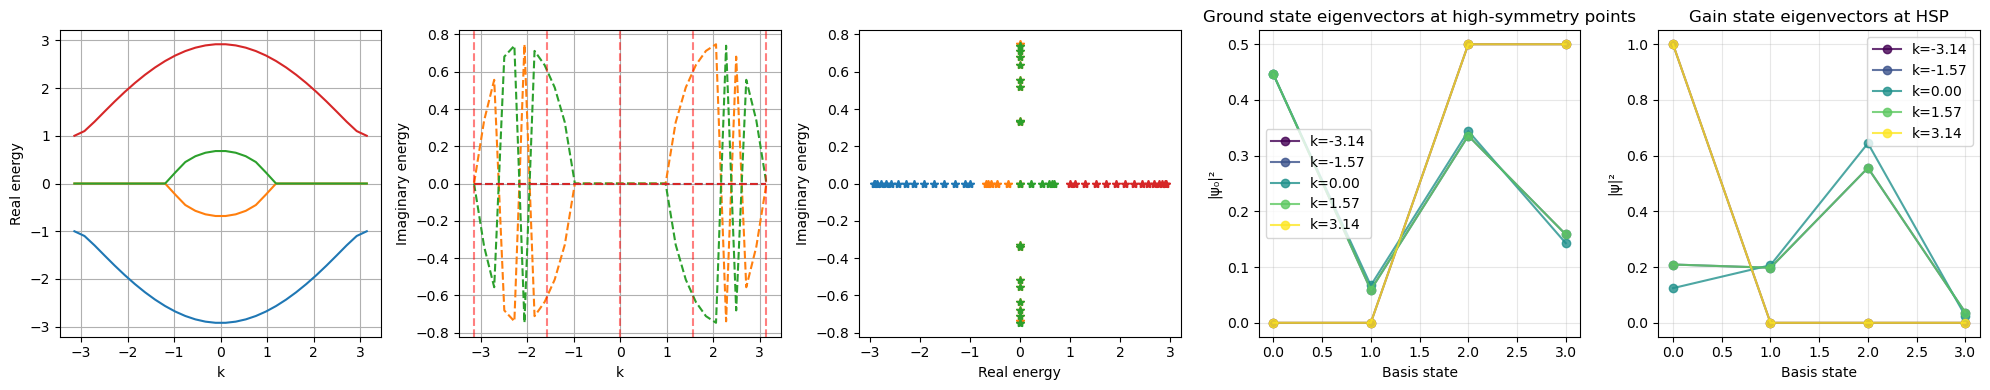
\includegraphics[width=\textwidth]{H-N_ladder_PBC_nonreciprocal.png}
%         \caption{Hatano-Nelson ladder PBC with non-reciprocal hopping.}
%     \end{figure}
% \end{frame}

% \begin{frame}[allowframebreaks]{Hatano-Nelson ladder OBC}
%     \begin{figure}
%         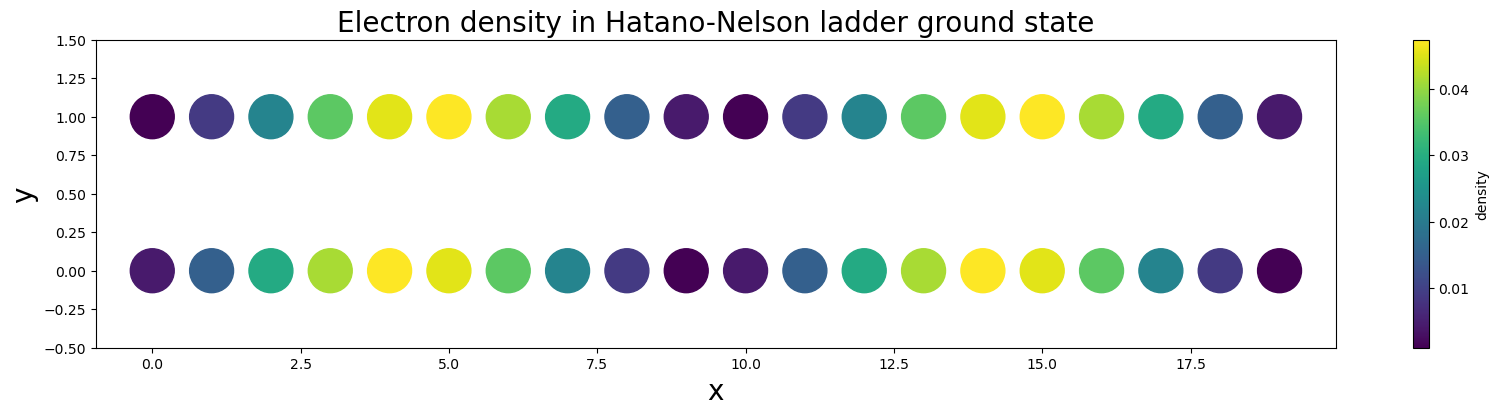
\includegraphics[width=\textwidth]{H-N_ladder_OBC_U=0.png}
%         \caption{Hatano-Nelson ladder OBC ordinary: U=0 and reciprocal hopping.}
%     \end{figure}
%     \framebreak
%     \begin{figure}
%         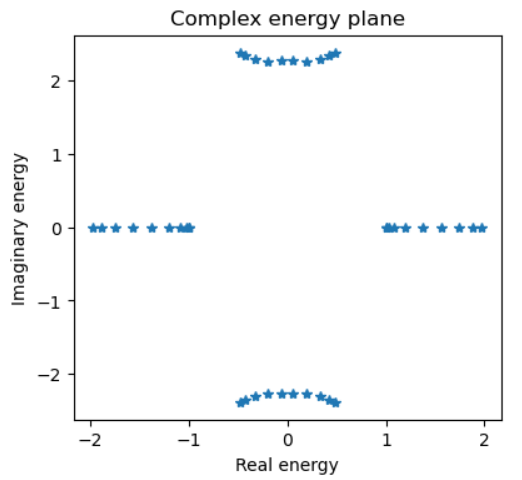
\includegraphics[width=0.5\textwidth]{H-N_ladder_OBC_spectrum_imag_pot.png}
%         \caption{Spectrum of Hatano-Nelson ladder OBC with imaginary onsite potential.}
%     \end{figure}
%     \framebreak
%     \begin{figure}
%         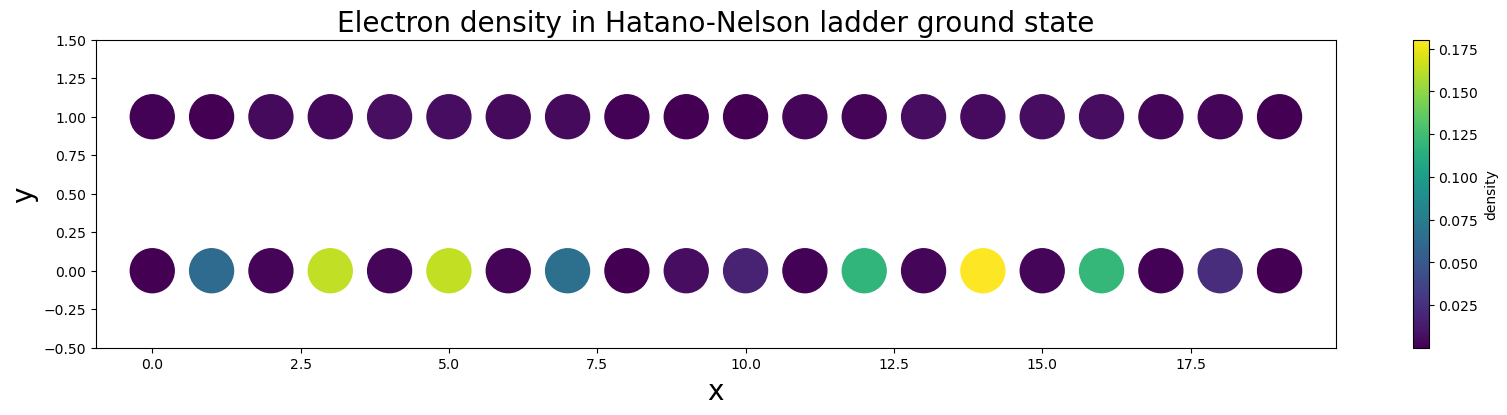
\includegraphics[width=\textwidth]{H-N_ladder_OBC_imag_pot.png}
%         \caption{Hatano-Nelson ladder OBC with imaginary onsite potential.}
%     \end{figure}
%     \framebreak
%     \begin{figure}
%         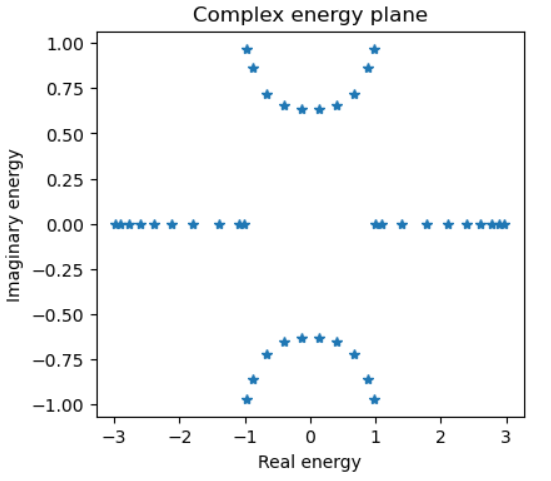
\includegraphics[width=0.5\textwidth]{H-N_ladder_OBC_spectrum_non_rec.png}
%         \caption{Spectrum of Hatano-Nelson ladder OBC with non-reciprocal hopping.}
%     \end{figure}
%     \framebreak
%     \begin{figure}
%         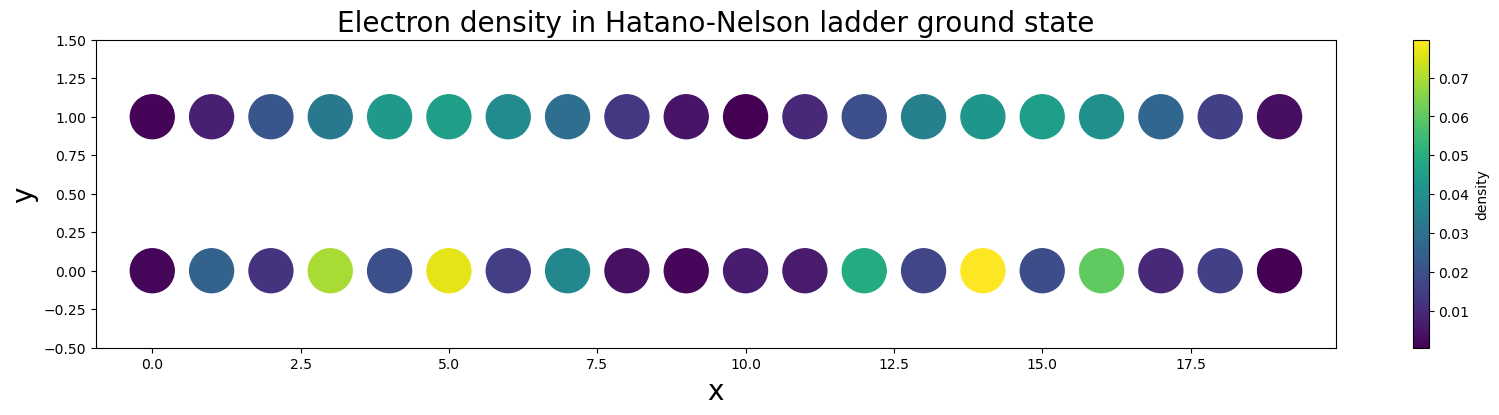
\includegraphics[width=\textwidth]{H-N_ladder_OBC_non_recipr.png}
%         \caption{Hatano-Nelson ladder OBC with non-reciprocal hopping.}
%     \end{figure}
% \end{frame}

% \begin{frame}[allowframebreaks]{Ongoing: bilayer Lieb lattice}
%     Stack Lieb lattices 
%     \begin{figure}
%         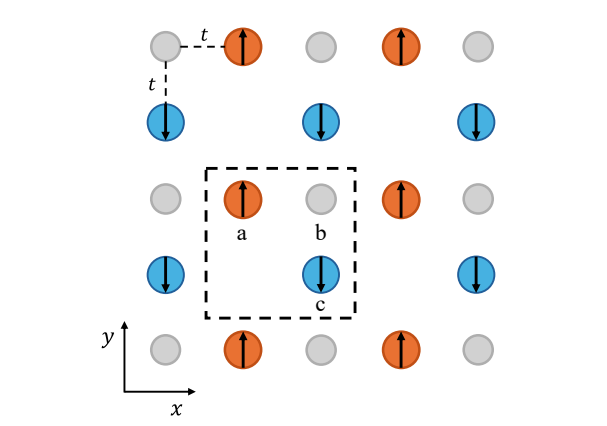
\includegraphics[width=0.5\textwidth]{Lieb_lattice.png}
%         \caption{\footfullcite{visser2023}}
%     \end{figure}
%     \begin{figure}
%         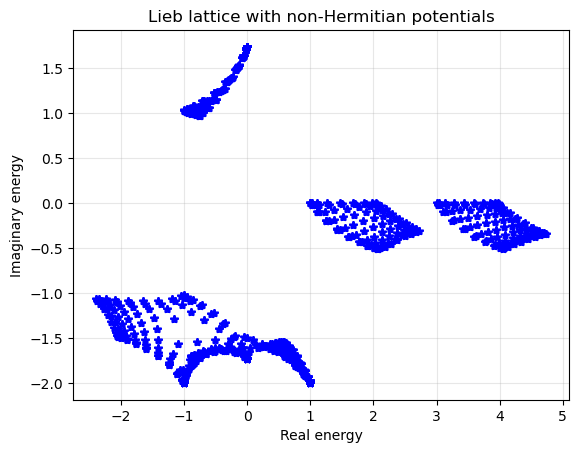
\includegraphics[width=0.5\textwidth]{bilayer_lieb_imaginarypot.png}
%         \caption{Spectrum of bilayer Lieb lattice with imaginary onsite potential.}
%     \end{figure}
% \end{frame}

% \begin{frame}{Summary}
%     \begin{alertblock}{Goal}
%         Study altermagnetism and non-hermiticity in classical analogues 
%     \end{alertblock}
%     \vfill
%     \begin{itemize}
%         \item Altermagnets: $C_4\mathcal{T}$ symmetry can lead to anisotropic and spin-momentum locking propagation \vfill
%         \item Non-hermitian skin effect: waves localized at boundaries \vfill
%         \item Classical analogues enable experimental realization
%     \end{itemize}
% \end{frame}

% \begin{frame}
%         \begin{tikzpicture}[
%     scale=1.3, transform shape,
%     >=stealth,
%     % Styles for stability tracking
%     stable/.style={line width=1.5pt, draw=blue!70!black},
%     unstable/.style={line width=1.5pt, dashed, draw=red!70!black},
%     surface/.style={fill=cyan!30, opacity=0.4}
% ]

%     % =========================================================================
%     % 1. COORDINATE AXES (3D Perspective)
%     % =========================================================================
%     \draw[->, thick] (-2.5, 0) -- (3.5, 0) node[right] {$\mu$}; % Parameter axis
%     \draw[->, thick] (0, -1.8) -- (0, 2.0) node[above] {$x$};   % State axis 1
%     \draw[->, thick] (0.8, 0.8) -- (-1.2, -1.2) node[below left] {$y$}; % State axis 2 (projected)

%     % Bifurcation label (Fixed the color typo here)
%     \node[above, font=\small, text=blue!70!black] at (0,0.1) {$\mu=0$};

%     % =========================================================================
%     % 2. PHASE SPACE REGIME: \mu < 0 (Stable Fixed Point)
%     % =========================================================================
%     \draw[stable] (-2.2, 0) -- (0, 0);
    
%     % Inward spiral representation to show stability trajectory
%     \draw[->, blue!60, line width=0.8pt, domain=0:3.5*pi, samples=100, smooth] 
%         plot ({-1.5 + 0.5*exp(-0.3*\x)*cos(\x r)}, {0.5*exp(-0.3*\x)*sin(\x r)});
%     \node[blue!80!black, font=\tiny] at (-1.5, 0.6) {Stable Focus};

%     % =========================================================================
%     % 3. PHASE SPACE REGIME: \mu > 0 (Unstable Center + Limit Cycle)
%     % =========================================================================
%     \draw[unstable] (0, 0) -- (3.0, 0);

%     % Outward spiral from origin to show instability trajectory
%     \draw[->, red!60, line width=0.8pt, domain=0:2.5*pi, samples=100, smooth] 
%         plot ({2.0 + 0.1*exp(0.25*\x)*cos(\x r)}, {0.1*exp(0.25*\x)*sin(\x r)});
%     \node[red!80!black, font=\tiny] at (2.0, 0.25) {Unstable};

%     % --- The 3D Parabolic Surface (Limit Cycles) ---
%     % Fixed the shading calculation here to avoid using "backward" or "name path"
%     \fill[surface] (0,0) parabola (2.8, 1.4) -- (2.8, -1.4) parabola (0,0);

%     % Redraw the profile lines on top of the shading so they stay crisp
%     \draw[stable] (0,0) parabola (2.8, 1.4);
%     \draw[stable] (0,0) parabola (2.8, -1.4);

%     % Cross-sectional Limit Cycle Rings at distinct \mu values
%     % Ring 1 (Midway \mu)
%     \draw[gray!60, thin] (1.3, 0) ellipse (0.15cm and 0.65cm); 
    
%     % Ring 2 (End of the paraboloid, bold stable limit cycle)
%     \draw[stable, fill=cyan!10, fill opacity=0.3] (2.8, 0) ellipse (0.25cm and 1.4cm);
    
%     % Draw an arrow along the limit cycle ring to show orbital direction
%     \draw[->, line width=1.2pt, blue!70!black] (2.8, 1.4) arc (90:45:0.25cm and 1.4cm);

%     % Labels for clarity
%     \node[blue!80!black, font=\small, text width=2cm, align=center] at (3.3, 1.5) {Stable\\Limit Cycle\\$r \propto \sqrt{\mu}$};

% \end{tikzpicture}
% \end{frame}



% \begin{frame}{References}
%     \bibliographystyle{plain} % or apsrev4-1, ieeetr, plain, etc.
%     \bibliography{bibliography}
%     \nofootfullcite{*}
% \end{frame}
\end{document}